\documentclass[letterpaper,12pt,oneside]{book}

% Language setting
% Replace `english' with e.g. `spanish' to change the document language
\usepackage[spanish]{babel}
\usepackage{amssymb, amsthm}
\usepackage[utf8]{inputenc}
\usepackage{bbm}
\usepackage{bm}
\usepackage[bb=dsserif]{mathalpha}
\usepackage{amsmath}
\usepackage{stackrel}
\usepackage{tikz}
\usepackage{graphicx}
\usepackage{caption}
\usepackage{kbordermatrix}
\usepackage{unicode-math}
\usepackage{dsfont}
\usepackage{geometry}
\geometry{left=4cm,right=2.5cm,top=2.5cm,bottom=2.5cm}
\usepackage{lineno}
\usepackage{textcomp}
\usepackage{fp}
\usepackage[backend=biber, style=numeric, citestyle=numeric, sorting=nyt, maxcitenames=1, maxbibnames=99]{biblatex}
\defbibheading{bibliography}[\refname]{}
\addbibresource{Bibliografia.bib}
\usetikzlibrary{shapes.geometric}


%\usepackage[vietnam]{babel}
\usepackage{xcolor,colortbl}
% Useful packages
\usepackage{amsmath}
\usepackage{graphicx}
\usepackage{hyperref}



\parindent = 0.5cm% Sangría de párrafo
\parskip 0.2cm% Salto entre párrafos
\renewcommand{\baselinestretch}{1.5}

\newcommand{\HRule}{\rule{\linewidth}{0.5mm}}% Linea Horizontal

% Color links
\hypersetup{
    colorlinks=true,
    linkcolor=red!70!black,      % Color de los enlaces a otras partes del documento (por ejemplo, \ref)
    citecolor=blue!70!black,    % Color de los enlaces a citas bibliográficas
    urlcolor=red!70!black,      % Color de los enlaces URL
}

\newcommand\Bbbbone{%
    \ifdefined\mathbbb%
        \mathbbb{1}%
    \else%
        \boldsymbol{\mathbb{1}}%
    \fi}

\newcommand{\hh}[1]{{\color{red} * #1 *}}
\newcommand{\fs}[1]{{\color{blue}* #1 *}}

%%%% Ajustamos el margen y el font de la descripción de cada figura.
\captionsetup[figure]{margin=50pt, justification=justified}

%%%%%%%%%%%%%%%%%%%%%%%%%%%%%%%%%%%%%%%%%%%%%
% Para teoremas, proposición y demnostración
\newtheorem{teorema}{Teorema}
\newtheorem{prop}[teorema]{Proposición}
\newtheorem{lema}[teorema]{Lema}
\newtheorem{corolario}[teorema]{Corolario}
\newtheorem{definicion}[teorema]{Definición}
%\newtheorem{}{}


% Creación de comandos %
\providecommand{\abs}[1]{\lvert#1\rvert}
\providecommand{\norm}[1]{\lVert#1\rVert}

\newcommand{\K}[2][5]{
    \begin{tikzpicture}
        \def\ang{360/#2}
        % Dibujar vértices como círculos negros
        \foreach \i in {1,...,#2}
            \node[fill=black, circle, inner sep=2pt, minimum size=4pt] at (\ang*\i:#1) {};
        % Dibujar aristas
        \foreach \i in {1,...,#2}
            \foreach \j in {1,...,#2}
                \draw (\ang*\i:#1) -- (\ang*\j:#1);
    \end{tikzpicture}
}




% Palabras recurrentes Chung,Graham y Wilson
\newcommand{\disc}{\mathrm{DISC}}
\newcommand{\discp}{\mathrm{DISC'}}
\newcommand{\Count}{\mathrm{COUNT}}
%\newcommand{\Cuatro}{\mathrm{COUNT}_{p,C_4}}
\newcommand{\codeg}{\mathrm{CODEG}}
\newcommand{\eig}{\mathrm{EIG}}

% Ahora para Chung-Graham y Wilson bipartito
\newcommand{\bidisc}{\mathrm{BI-DISC}}
\newcommand{\bicount}{\mathrm{BI-COUNT}}
\newcommand{\izcodeg}{\mathrm{IZQ-CODEG}}
\newcommand{\dercodeg}{\mathrm{DER-CODEG}}
\newcommand{\bieig}{\mathrm{BI-EIG}}

% Define codeg
\newcommand{\cod}{\mathrm{codeg}}
% Define Traza
\newcommand{\Tr}{\mathrm{Tr}}
% Define varianza
\newcommand{\var}{\mathrm{Var}}
%\documentclass[tikz, border = 10pt]{standalone}

\usepackage{pgfgantt}
%\def\proof{\paragraph{Demostraci\'on Segunda parte Teorema 3:\\}}
%\def\endproof{\hfill$\blacksquare$}

\newcommand{\prooftext}{}

\newenvironment{myproof}[1]
{
    \renewcommand{\prooftext}{#1}    
    \paragraph{\prooftext:}\par
}
{
    \hfill$\blacksquare$
    \renewcommand{\prooftext}{}
}


\usepackage{forloop}
\newcounter{loopcntr}
\newcommand{\rpt}[2][1]{%
    \forloop{loopcntr}{0}{\value{loopcntr}<#1}{#2}%
}
\newcommand{\on}[1][1]{
    \forloop{loopcntr}{0}{\value{loopcntr}<#1}{&\cellcolor{gray}}
}
\newcommand{\off}[1][1]{
    \forloop{loopcntr}{0}{\value{loopcntr}<#1}{&}
}

% Set page size and margins
% Replace `letterpaper' with `a4paper' for UK/EU standard size
%\usepackage[letterpaper,top=2cm,bottom=2cm,left=3cm,right=3cm,marginparwidth=1.75cm]{geometry}



\providecommand{\abs}[1]{\lvert#1\rvert}
\providecommand{\norm}[1]{\lVert#1\rVert}


\let\varepsilon=\varepsilon

\usetikzlibrary{backgrounds}


%% Lo de abajo es ultra temporal
\makeatletter
\newcommand{\canvaswidth}{12}
\newcommand{\canvasheight}{6}

\newcommand{\gettikzxy}[3]{ % I got this from http://tex.stackexchange.com/questions/33703/extract-x-y-coordinate-of-an-arbitrary-point-in-tikz
    \tikz@scan@one@point\pgfutil@firstofone#1\relax
    \edef#2{\the\pgf@x}
    \edef#3{\the\pgf@y}
}
\makeatother

\tikzstyle{node}=[circle, draw, thin,fill=cyan!20, scale=0.8]

\begin{document}
%\linenumbers

%%%%%%%%%%%%%%%%%%%%%%%%%%%%%%%%%%%%%%%%%%%%%%%%%%%%
%Portada
%%%%%%%%%%%%%%%%%%%%%%%%%%%%%%%%%%%%%%%%%%%%%%%%%%%%

\begin{titlepage}


\begin{figure}[ht]
\hspace{0.1\linewidth}
\begin{minipage}[b]{0.75\linewidth}
\begin{center}
\textbf{\Large{UNIVERSIDAD DE SANTIAGO DE CHILE}}\\
\textbf{FACULTAD DE CIENCIA}\\
\textbf{DEPARTAMENTO DE MATEMÁTICA Y CIENCIA DE LA COMPUTACIÓN}
\end{center}	
\end{minipage}
\begin{minipage}[b]{0.1\linewidth}
\centering

\includegraphics[width=2cm]{Imágenes/logo5}
\end{minipage}
\end{figure}

\begin{center}
\vspace{2.5cm}

% Título de Trabajo
\begin{center}
\Large{\textbf{Grafos cuasi-aleatorios y el Lema de regularidad de Szemerédi}}
\end{center}
\smallskip

% Nombre Autor
\begin{center}
{\textbf{Felipe Andrés Sánchez Erazo}}
\end{center}
\vspace{2.5cm}

% Profesor Guía
\hspace{0.45\linewidth}
\begin{minipage}[b]{0.45\linewidth}
\begin{flushleft}
\textbf{Profesor(a) Guía:}\\
Hi\d{ê}p Hàn
% si su tesis tiene profesor(a) co-guía, descomente las siguientes líneas
%\\
%\textbf{Profesor(a) Co-Guía:}\\
%escriba el nombre del profesor(a) co-guía.
\end{flushleft}
\end{minipage}

\vspace{2cm}

% Protocolo
\hspace{0.45\linewidth}
\begin{minipage}[b]{0.45\linewidth}
\begin{flushleft}
Trabajo de titulación para optar
al \\
título profesional de Ingeniero Matemático
\end{flushleft}
\end{minipage}

\vspace{1.5cm}

\begin{center}
Santiago - Chile \\
2024
\end{center}
%\setlinespacing{1.5}

\end{center}
\end{titlepage}
\pagenumbering{roman}
%%%%%%%%%%%%%%%%%%%%%%%%%%%%%%%%%%%%%%%%%%%%%%%%%%%%
%Derechos de Autor
%%%%%%%%%%%%%%%%%%%%%%%%%%%%%%%%%%%%%%%%%%%%%%%%%%%%
  © Felipe Andrés Sánchez Erazo. \\
Se  autoriza  la  reproducción  parcial  o  total  de  esta  obra  con  fines 
académicos,  por  cualquier  forma,  medio  o  procedimiento,  siempre  y 
cuando se incluya la cita bibliográfica del documento. 

\newpage


%%%%%%%%%%%%%%%%%%%%%%%%%%%%%%%%%%%%%%%%%%%%%%%%%%%%
%Hoja de Evaluación 
%%%%%%%%%%%%%%%%%%%%%%%%%%%%%%%%%%%%%%%%%%%%%%%%%%%%
%
%

\begin{figure}[ht]
\hspace{0.1\linewidth}
\begin{minipage}[b]{0.75\linewidth}
\begin{center}
\textbf{\Large{UNIVERSIDAD DE SANTIAGO DE CHILE}}\\
\textbf{FACULTAD DE CIENCIA}\\
\textbf{DEPARTAMENTO DE MATEMÁTICA Y CIENCIA DE LA COMPUTACIÓN}
\end{center}	
\end{minipage}
\begin{minipage}[b]{0.1\linewidth}
\centering

\includegraphics[width=2cm]{Imágenes/logo5}
\end{minipage}
\end{figure}

\begin{center}


% Título de Trabajo
\begin{center}
\Large{\textbf{Grafos cuasi-aleatorios y el Lema de regularidad de Szemerédi}}
\end{center}


% Nombre Autor
\begin{center}
{\textbf{Felipe Andrés Sánchez Erazo}}
\end{center}


\smallskip
\begin{center}
Trabajo de Titulación presentado a la Facultad de Ciencia, en cumplimiento parcial de los requisitos exigidos para optar al título de \textbf{Ingeniero Matemático}.\\
Este trabajo de Graduación fue presentado bajo la supervisión del profesor guía Dr. Hi\d{ê}p Hàn, 
%y del (de la) profesor(a) co-guía Dr. XXX
del Departamento de Matemática y Ciencia de la Computación de la Facultad de Ciencia.
\end{center}



\begin{center}
\hspace{0.45\linewidth}
\begin{minipage}[b]{0.9\linewidth}
\begin{flushright}
\begin{tabular}{lcr}
  &&\\
  & \hspace{2cm} & \rule{6cm}{1pt}\\
&\hspace{2cm}  & Dr. Hi\d{ê}p Hàn\\
  &&\textit{Profesor Guía}\\
  &&\\
%& \hspace{2cm} & \rule{6cm}{1pt}\\
%&\hspace{2cm}  & Dr(a). nombre profesor(a) co-guía.\\
% &&\textit{Profesor(a) Co-Guía}\\
%  &&\\
& \hspace{2cm} & \rule{6cm}{1pt}\\
&\hspace{2cm}&  Dr. Marcos Kiwi Krauskopf\\
&\hspace{2cm}&\textit{Profesor Informante}\\
  &&\\
\rule{5cm}{1pt} & \hspace{2cm} & \rule{6cm}{1pt}\\
Pablo Marín Álvarez&\hspace{2cm}&  Dr. Sebastián Barbieri Lemp\\
\textit{Director del Departamento}&&\textit{Profesor Informante}
\end{tabular}
\end{flushright}
\end{minipage}
\end{center}

\end{center}



\newpage



%%%%%%%%%%%%%%%%%%%%%%%%%%%%%%%%%%%%%%%%%%%%%%%%%%%%
% INFORMES DE TESIS
%%%%%%%%%%%%%%%%%%%%%%%%%%%%%%%%%%%%%%%%%%%%%%%%%%%%

%agregue aquí los informes realizados por la comisión
% use el comando includepdf  para tal efecto

%\includepdf[pages=-]{./Informe_tesis/Informe.pdf}
%\includepdf[pages=-]{.pdf}
%\includepdf[pages=-]{.pdf}
%\includepdf[pages=-]{.pdf}
%\includepdf[pages=-]{.pdf}


%\newpage








%%%%%%%%%%%%%%%%%%%%%%%%%%%%%%%%%%%%%%%%%%%%%%%%%%%%
%Dedicatoria
%%%%%%%%%%%%%%%%%%%%%%%%%%%%%%%%%%%%%%%%%%%%%%%%%%%%

\begin{flushright}
\ \vfil\vfil
\textit{A mi abuelo, Sergio Sánchez}
\end{flushright}
\newpage

%%%%%%%%%%%%%%%%%%%%%%%%%%%%%%%%%%%%%%%%%%%%%%%%%%%%
%Agradecimientos
%%%%%%%%%%%%%%%%%%%%%%%%%%%%%%%%%%%%%%%%%%%%%%%%%%%%
%\chapter{Agradecimientos}

%Dōmo arigatōgozaimasu!

\newpage

%%%%%%%%%%%%%%%%%%%%%%%%%%%%%%%%%%%%%%%%%%%%%%%%%%%%
%Tabla de contenidos
%%%%%%%%%%%%%%%%%%%%%%%%%%%%%%%%%%%%%%%%%%%%%%%%%%%%

% Construye los índices automáticamente
%\tableofcontents
%\listoftables
%\listoffigures


%%%%%%%%%%%%%%%%%%%%%%%%%%%%%%%%%%%%%%%%%%%%%%%%%%%%
%Resumen
%%%%%%%%%%%%%%%%%%%%%%%%%%%%%%%%%%%%%%%%%%%%%%%%%%%%
%\chapter{Resumen}


%%%%%%%%%%%%%%%%%%%%%%%%%%%%%%%%%%%%%%%%%%%%%%%%%%%%
%Introducción
%%%%%%%%%%%%%%%%%%%%%%%%%%%%%%%%%%%%%%%%%%%%%%%%%%%%
%\mainmatter% INDICA COMIENZO DE PARTE PRINCIPAL DE LA TESIS
%\chapter*{Introducción}
%\addcontentsline{toc}{chapter}{Introducción}




%\begin{titlepage}
%    \begin{center}
%
%        
\includegraphics[width=0.33\textwidth]{Imágenes/logo_usach.png}
%        \vspace{1.5cm}
%
%        \textbf{\LARGE Grafos cuasi-aleatorios y lema de regularidad de Szemerédi}
%
%        \vspace{0.5cm}
%
%        \vspace{1.5cm}
%
%        \textbf{\textbf{Estudiante:} \\Felipe Sánchez Erazo\\   \vspace{1.5cm} \textbf{Profesor %Guía:}   \vspace{0.5cm} \\ Dr. Hi\d{ê}p Hàn}
%
%        \vspace{1.cm}
%            
%\textbf{Tesis para optar al título de Ingeniero Matemático de la Universidad de Santiago de %Chile}\\      
%\vspace{0.5cm}
%
%Departamento de Matemática y Ciencia de la computación \\
%Universidad de Santiago de Chile \\
%%11 de Julio de 2022 
%\date{\today}
%            
%        \vspace{0.8cm}
%    
%            \vspace{0.5cm}
%
%    \end{center}
%\end{titlepage}
%
%%\tableofcontents
%\newpage
%\vspace*{\fill}
%\begin{center}
%    \emph{\Large A mi abuelo, Sergio Sánchez.}
%\end{center}
%\vspace*{\fill}
%\newpage

%%%% Agradecimientos
\chapter*{Agradecimientos}
\addcontentsline{toc}{chapter}{Agradecimientos}

Primero quiero agradecer a mi madre, por ser una figura y pilar fundamental en mi vida, que me ha brindado una comprensión y cariño que no se puede medir. A mi padre, por su apoyo completamente incondicional en todas las decisiones que he tomado, y por despertar mi curiosidad por los saberes de este mundo. A mi hermano, mi compañero de viaje, mi cómplice, gracias por traer alegrías a cada lugar que vas. Te amo y admiro mucho, y aunque este logro es personal, espero que solo sea uno de muchos en nuestro andar.

También agredecer a los otros miembros de mi familia, quienes en todo momento me dieron palabras de aliento, y que de algún u otro modo, fueron parte de mi motivación en la elaboración de esta tesis. 

Quiero dar una mención especial y profunda gratitud a mi amada, Lourdes. Sin su constante apoyo, los días habrían sido más grises en el desarrollo de este trabajo. Gracias por tu admirable empatía al entender mis problemas y tristezas, incluso cuando yo no les hallaba. Te agradezco por hacer que mis momentos de alegrías tengan muchos más colores.

Mil gracias a aquellas personas que fueron parte de mi etapa universitaria y de la vida, hicieron que la travesía estuviese llena de momentos bellos. En particular, agradecer a Rodrigo, infinito amigo,  quien ha estado en todos los momentos más importantes de mi vida, y esta vez no fue la excepción. Cristian, por mostrarme lo lindas que pueden ser las coincidencias en la vida y la amistad duradera que a veces traen consigo. Catalina, por el Apoyo, Risas, Afecto y Motivación en la recta final de este trabajo. Ailine, por nuestras conversaciones terapéuticas y todas las veces que me dijiste ``Amigo, tú puedes''. Camilo, por mostrarme que la amistad puede ir más allá que el ser compañeros de trabajo, por tu dedicación, y por ser un referente para mí como profesional.

Doy gracias a mis amistades de la música por mantener viva esta gran pasión que compartimos. En especial, a mis cofrades de la Tuna Mayor de Ciencia de la Universidad de Santiago de Chile. ¡Aúpa Tuna!.

Quiero agradecer a mi profesor guía Hi\d{ê}p Hàn por su buena disposición, paciencia, y su inmensa comprensión y calidad humana. Aprecio mucho las conversaciones de la vida que tuvimos tomando un café. Fue realmente un honor trabajar con usted.

Finalmente, agradezco al proyecto FONDECYT 1231599 por financiar esta tesis.

\vfill
\begin{quote}
    \emph{``Adiós, adiós, adiós, ciudad de mi querer, donde con ilusión mi carrera estudié. Adiós, mi universidad, cuyo reloj no volveré a escuchar...''}
\end{quote}


\tableofcontents
\addcontentsline{toc}{chapter}{\listfigurename}
\listoffigures


\mainmatter
\chapter*{Introducción}
\addcontentsline{toc}{chapter}{Introducción}

Los grafos cuasi-aleatorios y el Lema de regularidad de Szemerédi son dos líneas de estudio íntimamente relacionadas. A grandes rasgos, un grafo cuasi-aleatorio es un grafo determinista que muestra el comportamiento que se esperaría de su contraparte aleatoria. Aunque la noción de cuasi-aleatoriedad es un objeto de estudio interesante por sí mismo, ha revelado tener profundas conexiones en varias ramas de la matemática y ciencias de la computación.

Por su parte, el Lema de regularidad, establece que \emph{cualquier} grafo puede ser aproximado por un número \emph{constante} de grafos cuasi-aleatorios. Como los grafos son objetos considerados carentes de estructura, la conexión con cuasi-aleatoriedad nos permite transferir la intuición probabilista a problemas deterministas.
Fue desarrollada originalmente por Endre Szemerédi en 1975, introducida como una herramienta auxiliar para demostrar su famoso teorema sobre progresiones aritméticas en subconjuntos de enteros con densidad superior positiva. Hoy en día se ha singularizado como un potente instrumento con múltiples aplicaciones. Por este y otros aportes en la matemática, Szemerédi fue nombrado ganador del premio Abel en 2012.

Esta tesis tiene el objetivo de abordar los dos tópicos mencionados anteriormente. En el Capítulo~\ref{cuasi-aleatoriedad} se presenta y demuestra el célebre Teorema de Chung, Graham y Wilson, el cual entrega una extensa lista de propiedades equivalentes que caracterizan la idea de los grafos cuasi-aleatorios. El Capítulo~\ref{Sec. LRS} expone dos demostraciones del Lema de regularidad de Szemerédi; la versión clásica vía \emph{incremento de energía}, y otra usando un enfoque espectral. Seguido de esto, se estudia cómo usar el Lema de regularidad en dos resultados particulares, que serán utilizados independientemente para dar demostraciones combinatoriales del Teorema de Roth. Para desarrollar los tópicos mencionados, el Capítulo~\ref{Preliminares} entrega los conceptos y resultados necesarios. 

\chapter{Preliminares} \label{Preliminares}

Este capítulo proporciona una introducción concisa de los conceptos y terminologías que se utilizarán en esta tesis. La sección~\ref{Teoría de grafos} repasa las nociones más básicas de la teoría de grafos, otorgando una línea de base para el desarrollo del documento. En la sección~\ref{Teoría espectral} se repasan algunos conceptos y resultados clásicos del álgebra lineal para abordar las propiedades necesarias de la teoría espectral de grafos. Por último, la sección~\ref{Grafos aleatorios} contextualiza y motiva el contenido de la sección~\ref{cuasi-aleatoriedad}.

En muchos de los resultados de esta tesis, la \emph{desigualdad de Cauchy-Schwarz} (DCS) es un argumento fundamental en sus demostraciones. En particular, se emplearán dos variantes que se enunciarán a continuación. Primero, recuerde que la DCS establece que todo $\boldsymbol{a} = (a_1 ,...,a_k),\boldsymbol{b}=(b_1 ,...,b_k)\in\mathbb{R}^{k}$ satisfacen
\begin{equation}
    \sum_{i=1}^{k}a_{i}^{2}\sum_{i=1}^{k}b_i^{2} \geq \left( \sum_{i=1}^{k}a_{i}b_{i}\right)^{2}.
\end{equation}
Entonces, si $\boldsymbol{b} = (1,...,1)$, se obtiene la primera variante:
\begin{equation} \label{CS_versión1}
    \sum_{i=1}^{k}a_{i}^{2} \geq \frac{1}{k}\left( \sum_{i=1}^{k} a_{i}\right)^{2}.
\end{equation}
Adicionalmente, considerando los reales $\alpha_1,...,\alpha_k > 0$ y $\beta_1,...\beta_k \geq 0$, defina $a_i = \sqrt{\alpha_i}$ y $b_i = \frac{\beta_i}{\sqrt{\alpha_i}}$ para conseguir la segunda variante:
\begin{equation} \label{Desigualdad_from_CS}
    \sum_{i=1}^{k} \frac{\beta_{i}^{2}}{\alpha_i} \geq \frac{\left( \sum_{i = 1}^{k} \beta_i\right)^{2}}{\sum_{i=1}^{k}\alpha_i}.
\end{equation}
Por otro lado, será usual utilizar la notación asintótica. Por esto, se define la notación considerando $f,g\not=0$ como funciones de $n$:
\begin{itemize}
    \item Si $\displaystyle\lim_{n\to\infty}f(n)/g(n)\to 0$, se dice que $f=o(g)$.
    \item Si $\displaystyle\lim_{n\to\infty}f(n)/g(n) < \infty$, se dice que $f=O(g)$. 
\end{itemize}

\section{Teoría de grafos} \label{Teoría de grafos}

Se denota al conjunto de los primeros $n$ naturales por $[n]:=\lbrace 1,2,...,n\rbrace$. También, si $S$ es un conjunto finito y $r$ es un entero positivo, se establece $\tbinom{S}{r}$ como el conjunto de todos los subconjuntos de $r$ elementos de $S$.
%%%% Definir grafo
Un \textbf{grafo} es un par $G = (V,E)$, donde $V$ representa el conjunto de \textbf{vértices}, y $E\subseteq \tbinom{V}{2}$ el conjunto de \textbf{aristas}. Para representar una arista, escribiremos $uv$ en vez de $\lbrace u,v\rbrace$. Dado un grafo $G$, denotamos por $V(G)$ a su conjunto de vértices, $E(G)$ a su conjunto de aristas, y $e_G := |E(G)|$ a la cantidad de aristas presentes en el grafo.
\begin{figure}[h]%%%% Ejemplo grafo
    \centering
    \begin{tikzpicture}[scale=1.3]
        % vértices
        \node[fill=black, circle, inner sep=1pt, minimum size=4pt, label={180:$\mathbf{2}$}] (2) at (-1.5, 0) {};
        \node[fill=black, circle, inner sep=1pt, minimum size=4pt, label={180:$\mathbf{1}$}] (1) at (-1.5, -1.5) {};
        \node[fill=black, circle, inner sep=1pt, minimum size=4pt, label={0:$\mathbf{3}$}] (3) at (0, 0) {};
        \node[fill=black, circle, inner sep=1pt, minimum size=4pt, label={0:$\mathbf{5}$}] (5) at (1.8, 0) {};
        \node[fill=black, circle, inner sep=1pt, minimum size=4pt, label={0:$\mathbf{4}$}] (4) at (1.8, -1.5) {};

        % aristas
        \draw[line width=1.2] (1) -- (2);
        \draw[line width=1.2] (2) -- (3);
        \draw[line width=1.2] (1) -- (3);
        \draw[line width=1.2] (5) -- (4);
    \end{tikzpicture}
    \caption[Ejemplo de un grafo]{Ejemplo de un grafo con conjunto de vértices $V = \lbrace 1,2,3,4,5\rbrace$ y conjunto de aristas $E =  \lbrace 12, 23, 13, 45\rbrace$.}
\end{figure} 
Si $G = (V,E)$ es un grafo cualquiera y $u,v\in V$, se dirá que $u$ es \textbf{adyacente} a $v$ (o viceversa) si y solamente si $uv\in E$. Si $X,Y\subset V$ son dos subconjuntos no necesariamente disjuntos, se define la cantidad de tuplas que forman una arista de la siguiente manera:
\begin{equation} \label{eq e(X,Y)}
    e(X,Y) := \Big|\lbrace (x,y)\in X\times Y : xy\in E\rbrace\Big|.
\end{equation}
Cuando $X\cap Y = \emptyset$, $e(X,Y)$ cuenta el número de aristas entre $X$ e $Y$, y cuando $X\cap Y\not=\emptyset$, $e(X,Y)$ realiza un doble conteo sobre las aristas que se encuentran en $X\cap Y$. Además, por lo anterior, se define naturalmente $e(X) = \frac{e(X,X)}{2}$.

Se entenderá por \textbf{vecindad} de $u\in V$ como el conjunto de todos los vértices adyacentes a $u$, es decir,
\begin{equation} \label{vecindad}
    N(u) := \lbrace v\in V(G) : uv\in E(G)\rbrace.
\end{equation}
Si $\mathbbm{1}_{X}$ denota la función indicatriz de un conjunto $X$, se define el \textbf{grado} de un vértice $u\in V$ con respecto a algún subconjunto de vértices $Y\subseteq V$ de la siguiente manera:
\begin{equation*}
    \deg(u;Y) := \sum_{v\in Y} \mathbbm{1}_{E}(uv) = |N(u)\cap Y|.
\end{equation*}
En particular, cuando $Y=V$,
\begin{equation*}
    \deg(u) = \sum_{v\in V} \mathbbm{1}_{E}(uv) = |N(u)|.
\end{equation*}
Una propiedad elemental en teoría de grafos es la relación que guarda la suma del grado de todos los vértices y la cantidad de aristas de un grafo.
\begin{prop} %%%% Suma grados = 2e
    Dado un grafo $G = (V,E)$, entonces
    \begin{equation}
        \sum_{u\in V}\deg (u) = 2e_G.
    \end{equation}
\end{prop} %%%% Demostración suma grados = 2e
\begin{proof}
    Cada arista $uv\in E$ será contada dos veces en la suma, una contribución por $u$, y otra por $v$.
\end{proof}
En algunas ocasiones estaremos interesados en la cantidad de vecinos que comparten dos vértices del grafo $G = (V, E)$. Entonces, se define el \textbf{cogrado} de un par de vértices $u,v\in V$ no necesariamente diferentes mediante:
\begin{equation*}
    \cod(u,v) = \sum_{w\in V} \mathbbm{1}_{E}(wu) \mathbbm{1}_{E}(wv)=|N(u)\cap N(v)|.
\end{equation*}
Mostraremos que existe una relación intrínseca entre los conceptos de grado y cogrado, la cual será de utilidad en la sección~\ref{cuasi-aleatoriedad}.
\begin{prop} \label{Prop: grado-cogrado} %%%% Proposición: Relación grado-cogrado
    Sea $G = (V,E)$ un grafo e $Y\subset V$ un subconjunto de vértices, entonces
    \[
        \sum_{u\in V} \deg(u;Y)^{2} =  \sum_{v\in Y}\sum_{v'\in Y}\cod(v,v').
    \]
\end{prop}
\begin{proof} %%%% Demostración Proposición: Relación grado-cogrado
    Utilizando las respectivas definiciones de grado y cogrado, el resultado se obtiene de seguir el siguiente cálculo:
    \begin{align*}
        \sum_{u\in V} \deg(u;Y)^{2} &= \sum_{u\in V}\sum_{v\in Y}\sum_{v'\in Y} \mathbbm{1}_{E}(uv) \mathbbm{1}_{E}(uv')\\
        &= \sum_{v\in Y}\sum_{v'\in Y}\sum_{u\in V} \mathbbm{1}_{E}(vu) \mathbbm{1}_{E}(v'u)\\
        &= \sum_{v\in Y}\sum_{v'\in Y}\cod(v,v').
    \end{align*}
\end{proof}
Observe que en particular, cuando $Y=V$, se satisface
\begin{equation} \label{grado-cogrado}
    \sum_{u\in V} \deg(u)^{2} = \sum_{u\in V}\sum_{v\in V}\cod(u,v).
\end{equation}
A continuación, se enuncian algunos grafos especiales que son contemplados en esta tesis. Diremos que un grafo $G = (V,E)$ es $k$-\textbf{partito} si $V$ se puede dividir en $k$ subconjuntos disjuntos $V_1,V_2,...,V_k$ tales que si $uv\in E$ entonces $u\in V_i$ y $v\in V_j$, con $i\not=j$. En particular, a un grafo $2$-partito lo llamaremos \textbf{bipartito}.

\begin{figure}[h] %%%% Ejemplo grafo 3-partito
    \centering
    \begin{tikzpicture}[scale=1.3]
        % Conjunto 1
        \foreach \x in {1,2,3}
            \node[fill=black, circle, inner sep=2pt, minimum size=4pt] (A\x) at (\x,2) {};

        % Conjunto 2
        \foreach \y in {1,2,3,4}
            \node[fill=black, circle, inner sep=2pt, minimum size=4pt] (B\y) at (\y-0.5,0) {};

        % Conjunto 3
        \foreach \z in {1,2,3}
            \node[fill=black, circle, inner sep=2pt, minimum size=4pt] (C\z) at (\z+1, -2) {};

        % Conexiones
        \draw (A1) -- (B1);
        \draw (A2) -- (B2);
        \draw (A3) -- (B3);
        \draw (A2) -- (B4);
        
        \draw (B1) -- (C2);
        \draw (B2) -- (C3);
        \draw (B3) -- (C1);

        \draw (C1) -- (A2);
        \draw (C2) -- (A3);
        \draw (C3) -- (A1);
    \end{tikzpicture}
    \caption[Ejemplo de un grafo 3-partito]{Ejemplo de un grafo 3-partito.}
\end{figure}

Un \textbf{grafo completo} de $n$ vértices, denotado por $K_n$, es un grafo en el cual todos sus vértices son adyacentes entre ellos, es decir, todo par de vértices en el grafo posee una arista que los conecta. Similarmente, se denota por $K_{n,m}$ al \textbf{grafo bipartito completo} con $n$ y $m$ elementos en sus respectivos conjuntos de vértices. Observe que la cantidad de aristas en los grafos anteriores son exactamente $e_{K_n} = \tbinom{n}{2}$ y $e_{K_{n,m}} = n\cdot m$. Por último, un grafo $d$-\textbf{regular} es aquel que presenta todos sus vértices con grado $d$.

\begin{figure}[h] % Ejemplos grafos especiales
    \centering
    \begin{tikzpicture}[scale=1.2]
        \begin{scope}[shift={(0,0)}] % NO PUEDO CORRERLO UN POQUITO A LA IZQ.
            % Grafo completo: K_6
        \K[1.6]{6}    
        \end{scope}

        \begin{scope}[shift={(-2cm,0)}]
            % Grafo completo bipartito: K_{3,5}
            % Definir los vértices de la primera bipartición (A)
            \foreach \i in {1,2,3}{
                \node[fill=black, circle, inner sep=2pt, minimum size=4pt] (A\i) at (-1,\i -0.7) {};
            }
        

            % Definir los vértices de la segunda bipartición (B)
            \foreach \i in {1,...,5}{
                \node[fill=black, circle, inner sep=2pt, minimum size=4pt] (B\i) at (1,\i - 0.5 - 1.3) {};
            }
        

            % Conectar cada nodo de A con cada nodo de B
            \foreach \i in {1,2,3}{
                \foreach \j in {1,...,5}{
                    \draw (A\i) -- (B\j);
                }
            }
        \end{scope}
        
        \begin{scope}[shift={(6cm,1.4cm)}]
            % Grafo 3-regular
            \foreach \x [count=\i] in {18,90,162,234,306}{
                \coordinate (i\i) at (\x:1cm) {};
                \coordinate (o\i) at (\x:1.8cm) {};
                \draw (\x:1cm) -- (\x:1.8cm);
            }

            \draw (o1) -- (o2) -- (o3) -- (o4)-- (o5)--(o1);
            \draw (i1) -- (i3) -- (i5) -- (i2)-- (i4)--(i1);

            \foreach \x [count=\i] in {18,90,162,234,306}{
                \node[fill=black, circle, inner sep=2pt, minimum size=4pt] at (\x:1cm){};
                \node[fill=black, circle, inner sep=2pt, minimum size=4pt] at (\x:1.8cm){};
            }  
        \end{scope}
    \end{tikzpicture}
    \caption[Ejemplos de un grafo especial $K_{3,5}$, $K_6$ y $3$-regular]{Ejemplo de los grafos especiales $K_{3,5}$, $K_6$ y 3-regular.}
\end{figure} 
%%%% Definición caminata, caminata cerrada, camino y ciclos
Otro término relevante en este trabajo son las diferentes nociones de rutas que se pueden encontrar siguiendo una determinada secuencia de aristas en un grafo. Suponga que el grafo $G$ posee $n\geq k$ vértices, entonces se definen los siguientes conceptos:
\begin{itemize}
    % Caminata
    \item Una \textbf{caminata}, es una secuencia de vértices no necesariamente distintos \newline $v_0,v_1,...,v_k$ tales que $v_{i-1}v_{i}\in E(G)$ para todo $i\in [k]$. Si $v_0 = v_k$, se dice que es una \textbf{caminata cerrada}. El \textbf{largo} de una caminata está determinado por la cantidad de aristas que esta posea.
    % Camino
    %\item Un \textbf{camino} es una caminata con todos los vértices $v_i$ distintos.
    % Ciclo
    \item Un \textbf{ciclo}, es una caminata con $k\geq 2$ vértices únicos a excepción de $v_k$, que coincide con $v_0$. Se denotará por $C_k$ al ciclo de largo $k$.
\end{itemize}

\begin{figure}[h] % Ejemplos de caminata, camino y ciclo.
    \centering
    % minipage de grafo
    \begin{minipage}{0.35\textwidth}
        \centering
        \begin{tikzpicture}[scale=1.2]
            % vértices
            \node[fill=black, circle, inner sep=2pt, minimum size=4pt, label={90:$\mathbf{2}$}] (2) at (-0.8,0.4) {};
            \node[fill=black, circle, inner sep=2pt, minimum size=4pt, label={0:$\mathbf{3}$}] (3) at (0.8, 0.4) {};
            \node[fill=black, circle, inner sep=2pt, minimum size=4pt, label={270:$\mathbf{5}$}] (5) at (-0.8,-1.2) {};
            \node[fill=black, circle, inner sep=2pt, minimum size=4pt, label={0:$\mathbf{6}$}] (6) at (0.8,-1.2) {};

            \node[fill=black, circle, inner sep=2pt, minimum size=4pt, label={180:$\mathbf{1}$}] (1) at (-2,1.1) {};
            \node[fill=black, circle, inner sep=2pt, minimum size=4pt, label={180:$\mathbf{4}$}] (4) at (-2,-1.9) {};

            % Aristas
            \draw[line width=1.2] (1) -- (2) -- (3) -- (6) -- (5) -- (4);
            \draw[line width=1.2] (5) -- (2);
        \end{tikzpicture}
    \end{minipage}
    % minipage ejemplos concretos
    \begin{minipage}{0.15\linewidth}
        \begin{align*}
            &125456 \equiv \text{caminata de largo 5.}\\
            %&\\
            %&1236 \equiv \text{camino de largo 3.}\\
            &\\
            &23652 \equiv \text{ciclo de largo 4.}
        \end{align*}
    \end{minipage}
    \caption[Ejemplo de una caminata y un ciclo en un grafo]{Ejemplo de una caminata y un ciclo.}
    \label{ej caminos}
\end{figure}
\newpage
Por otro lado, para estudiar posteriormente relaciones estructurales entre grafos, se define un \textbf{isomorfismo} entre los grafos $H$ y $G$ como una biyección $f: V(H)\to V(G)$ tal que $uv\in E(H)$ si y solamente si $f(u)f(v)\in E(G)$. Si existe tal biyección, diremos que $H$ y $G$ son isomorfos.

Finalmente, se define una \textbf{copia etiquetada} de un grafo $H$ en $G$, como la aplicación inyectiva $f: V(H)\to V(G)$ tal que $f(u)f(v)\in E(G)$ cada vez que $uv\in E(H)$. En otras palabras, es un mapeo de los vértices de $H$ a los de $G$ que preserva las aristas. Se denotará por $\tbinom{G}{H}$ al conjunto de copias etiquetadas de $H$ en $G$.

\begin{figure}[h]
    \centering
    \begin{minipage}{0.49\linewidth}
        \centering
        % G_1
        \begin{tikzpicture}[baseline,scale=1]
            %\draw[step=0.5cm, gray, very thin] (-3,-3) grid (3,3);
            % Comienza ecuación
            \node at (-3,0) {$H=$};
            % Vértices 
            \node[fill=black, circle, inner sep=2pt, minimum size=4pt, label={180:$\mathbf{3}$}]  (3) at (-1.5,0) {};
            \node[fill=black, circle, inner sep=2pt, minimum size=4pt, label={0:$\mathbf{4}$}]  (4) at (1.5,0) {};
            \node[fill=black, circle, inner sep=2pt, minimum size=4pt, label={90:$\mathbf{1}$}]  (1) at (0,1.7) {};
            \node[fill=black, circle, inner sep=2pt, minimum size=4pt, label={270:$\mathbf{5}$}]  (5) at (0,-2) {};
            \node[fill=black, circle, inner sep=2pt, minimum size=4pt, label={90:$\mathbf{2}$}]  (2) at (3,2) {};
            % Aristas
            \draw[line width=1.2] (3) -- (1) -- (4) -- (2);
            \draw[line width=1.2] (1) -- (5);
        \end{tikzpicture}
    \end{minipage}
    \hfill
    \begin{minipage}{0.49\linewidth}
        \centering
        % G_2
        \begin{tikzpicture}[baseline,scale=1]
            \node at (-3,0) {$G=$};
            % Vértices
            \node[fill=black, circle, inner sep=2pt, minimum size=4pt, label={180:$\mathbf{b}$}]  (b) at (-1.5,0) {};
            \node[fill=black, circle, inner sep=2pt, minimum size=4pt, label={0:$\mathbf{d}$}]  (d) at (1.5,0) {};
            \node[fill=black, circle, inner sep=2pt, minimum size=4pt, label={90:$\mathbf{a}$}]  (a) at (0,1.7) {};
            \node[fill=black, circle, inner sep=2pt, minimum size=4pt, label={270:$\mathbf{e}$}]  (e) at (0,-2) {};
            \node[fill=black, circle, inner sep=2pt, minimum size=4pt, label={270:$\mathbf{c}$}]  (c) at (0,0) {};
            % Aristas
            \draw[line width=1.2] (e) -- (b) -- (a) -- (d) -- (e);
            \draw[line width=1.2] (a) -- (c);
        \end{tikzpicture}
    \end{minipage}
    \caption[Ejemplo de una copia etiquetada]{Ejemplo de una copia etiquetada de $H$ en $G$ mediante la función $f : V(H)\to V(G)$ definida por $f(1)=a$, $f(2)=e$, $f(3)=c$, $f(4)=b$ y $f(5)=d$.}
\end{figure}

\section{Álgebra lineal y teoría espectral de grafos} \label{Teoría espectral}

Se define $\mathcal{M}_{n\times m}(\mathbb{R})$ como el conjunto de matrices reales de $n$ filas y $m$ columnas, y denotaremos $A^{T}$ a la matriz traspuesta de $A\in\mathcal{M}_{n\times m}(\mathbb{R})$. También, representaremos por $\boldsymbol{1}$ $\in\mathcal{M}_{n\times 1}(\mathbb{R})$ al vector de solo $1$-entradas, $J\in\mathcal{M}_{n\times n}(\mathbb{R})$ a la matriz de solo $1$-entradas, $I_n\in \mathcal{M}_{n\times n}(\mathbb{R})$ a la matriz identidad, y $\boldsymbol{e}_i\in\mathcal{M}_{n\times 1}(\mathbb{R})$ como el vector de la base canónica de $\mathbb{R}^{n}$ con entrada $1$ en la posición $i$. Además, $\norm{\cdot}$ y $\langle \cdot, \cdot\rangle$ representarán en todo momento la norma y producto interno euclideano de $\mathbb{R}^{n}$ ($\mathbb{C}^{n}$, según corresponda) respectivamente.

Considerando una matriz cuadrada $A\in \mathcal{M}_{n\times n}(\mathbb{R})$, se define la \textbf{traza} de $A$ como la suma de los elementos de su diagonal principal. Esto es,
\begin{equation*}
    \Tr(A) = a_{11} + a_{22} + ... + a_{nn}.
\end{equation*}
Si $A,B\in\mathcal{M}_{n\times n}(\mathbb{R})$, entonces la traza resulta invariante bajo el orden de multiplicación de dichas matrices. En efecto, 
\begin{equation*}
    \Tr(AB) = \sum_{i=1}^{n}\left( \sum_{j=1}^{n} a_{ij}b_{ji}\right) = \sum_{j=1}^{n}\left( \sum_{i=1}^{n} a_{ij}b_{ji}\right) = \Tr(BA).
\end{equation*}
Una manera muy útil de representar un grafo es mediante una matriz cuadrada binaria, en la que sus filas y columnas representarán todos los vértices del grafo. La matriz adopta el valor $1$ en las coordenadas en que sus respectivos vértices forman una arista, y $0$ cuando no. Bajo esta representación, se consigue una visión clara y eficiente entre las relaciones de los vértices del grafo y se goza de las propiedades que ofrece el álgebra lineal.
\begin{definicion} \label{matriz_adyacencia} %%%% Definición formal matriz de adyacencia
    Dado un grafo $G$ sobre $n$ vértices, se define su \textbf{matriz de adyacencia} $A_{G}\in \mathcal{M}_{n\times n}(\mathbb{R})$ de la siguiente manera:
    \begin{equation*}
        a_{ij} =
        \begin{cases}
            1 & \mathrm{si}\  ij\in E(G),\\
            0 & \mathrm{en\ otro\ caso.}
        \end{cases}
    \end{equation*}
    Cuando el contexto sea claro, la matriz de adyacencia será representada simplemente por $A$.
\end{definicion}
%%%% Ejemplo de matriz de adyacencia de un grafo.
\renewcommand{\kbldelim}{(}
\renewcommand{\kbrdelim}{)}
\begin{figure}[h]
    \centering
    % Grafo
    \begin{minipage}{0.49\linewidth}
        \centering
        \begin{tikzpicture}[scale=1.2]
            \node at (-2.5,-1.1) {$G = $};
            % Vértices
            \node[fill=black, circle, inner sep=2pt, minimum size=4pt, label={270:$\mathbf{3}$}] (3) at (-0.5, -0.7) {};
            \node[fill=black, circle, inner sep=2pt, minimum size=4pt, label={290:$\mathbf{4}$}] (4) at (1.5, -0.7) {};
            \node[fill=black, circle, inner sep=2pt, minimum size=4pt, label={90:$\mathbf{1}$}] (1) at (-1, 0.8) {};
            \node[fill=black, circle, inner sep=2pt, minimum size=4pt, label={90:$\mathbf{2}$}] (2) at (2, 0.8) {};
            \node[fill=black, circle, inner sep=2pt, minimum size=4pt, label={270:$\mathbf{5}$}] (5) at (-1.5, -1.7) {};
            \node[fill=black, circle, inner sep=2pt, minimum size=4pt, label={270:$\mathbf{6}$}] (6) at (1, -2.2) {};
            % Aristas
            \draw[line width=1.2] (1) -- (2) -- (4) -- (3) -- (1) -- (5) -- (3);
            \draw[line width=1.2] (1) -- (4) -- (6) -- (3);
        \end{tikzpicture}
    \end{minipage}
    \hfill
    % Matriz
    \begin{minipage}{0.49\linewidth}
        \centering
        \begin{equation*}
            A_G = \kbordermatrix{
                & \mathbf{1} & \mathbf{2} & \mathbf{3} & \mathbf{4} & \mathbf{5} & \mathbf{6} \\
                \mathbf{1} & 0 & 1 & 1 & 1 & 1 & 0 \\
                \mathbf{2} & 1 & 0 & 0 & 1 & 0 & 0 \\
                \mathbf{3} & 1 & 0 & 0 & 1 & 1 & 1 \\
                \mathbf{4} & 1 & 1 & 1 & 0 & 0 & 1 \\
                \mathbf{5} & 1 & 0 & 1 & 0 & 0 & 0 \\
                \mathbf{6} & 0 & 0 & 1 & 1 & 0 & 0
            }
        \end{equation*}
    \end{minipage}
    \caption[Ejemplo de la matriz de adyacencia de un grafo]{Ejemplo de la representación de un grafo mediante la matriz de adyacencia.}
\end{figure}

Observe que la construcción anterior resulta siempre en una matriz simétrica, es decir, $A_{G}^{T} = A_{G}$. Además, a partir de todo grafo $G = ([n], E)$ con matriz de adyacencia $A$, se puede obtener un vector con los grados de todos los vértices del grafo aplicando el operador $A$ al vector de 1-entradas: 
\begin{equation} \label{A1=Mdeg}
    A\boldsymbol{1} = 
    \begin{pmatrix}
        \deg(1) \\
        \vdots \\
        \deg(n)
    \end{pmatrix}.
\end{equation}
Otro aspecto interesante de la matriz de adyacencia que será de utilidad en la sección~\ref{Sec. LRS}, es que nos permite reescribir la ecuación~\eqref{eq e(X,Y)} en función de ella. Para ver esto, considere la matriz de adyacencia $A$ del grafo $G = ([n], E)$, y los vértices $i,j\in [n]$. Luego, según la Definición~\ref{matriz_adyacencia},
\begin{equation*}
    e(\lbrace i\rbrace, \lbrace j\rbrace) = \boldsymbol{e}_i^{T} A \boldsymbol{e}_{j} = a_{ij}.
\end{equation*}
Y así, por linealidad, se extiende el resultado anterior sobre cualquier conjunto $X,Y\subset [n]$.
\begin{equation} \label{e(X,Y)=espectral}
    e(X,Y) = \sum_{i\in X}\sum_{j\in Y} \boldsymbol{e}_{i}^{T} A \boldsymbol{e}_{j} = \boldsymbol{v}_{X}^{T} A \boldsymbol{v}_{Y}.
\end{equation}
En la ecuación anterior, y desde ahora en adelante, el vector $\boldsymbol{v}_{X} = \sum_{i\in X}\boldsymbol{e}_{i}$ representa el vector indicador del subconjunto de vértices $X\subset [n]$ de algún grafo $G=([n], E)$.

Es importante destacar que la matriz de adyacencia no solo describe las conexiones entre cada par de vértices en un grafo, sino que también revela la cantidad exacta de caminatas que existen entre dos vértices de un largo determinado. En específico, la posición $ij$ de la $t$-ésima potencia de la matriz de adyacencia de un grafo guarda la cantidad de caminatas de largo $t$ entre los vértices $i$ y $j$.
\begin{prop} \label{potencia_matriz_adyacencia = caminatas} %%%% Lema: Potencia matriz de adyacencia
    Sea $t\geq 1$ un entero, y $A$ la matriz de adyacencia del grafo $G=([n], E)$. La $(i,j)$~-ésima entrada $a_{ij}^{(t)}$ de $A^{t}$, cuenta la cantidad de caminatas de largo $t$ que comienzan y terminan en los vértices $i$ y $j$ respectivamente.
\end{prop}
\begin{proof} %%%% Demostración Lema : Potencia matriz de adyacencia
    Cuando $t=1$, existe una caminata de largo $1$ que conecta los vértices $i$ y $j$ si y solamente si $a_{ij}^{(1)} = 1$. Ahora, asuma que el enunciado se cumple para algún $t > 1$ fijo. Note que cualquier caminata de largo $t+1$ entre $i$ y $j$ contiene una caminata de largo $t$ desde $i$ hasta un vecino de $j$, digamos $k$. Entonces si $k\in N(j)$, por la asunción del enunciado, el número de caminatas de largo $t$ entre $i$ y $k$ es $a_{ik}^{(t)}$. Por lo tanto, el número total de caminatas de largo $t+1$ desde $i$ hasta $t$ es exactamente
    \begin{equation*}
        \displaystyle\sum_{k\in V} a_{ik}^{(t)}\mathbbm{1}_{N(j)}(k) = \displaystyle\sum_{\ell=1}^{n}a_{i\ell}^{(t)}a_{\ell j} = a_{ij}^{(t+1)}.
    \end{equation*}
\end{proof}
Como consecuencia de la proposición anterior, en cualquier grafo $G = ([n], E)$ con matriz de adyacencia $A$, se puede representar la cantidad total de caminatas cerradas de largo $t$ en el grafo por medio de la traza, $\Tr(A^{t}) = \sum_{i=1}^{n}a_{ii}^{(t)}$. Con esto, note que $\Tr(A^{2}) = 2e_G$.

Por otro lado, para introducir algunos aspectos de la teoría espectral de grafos, recuerde que el vector no nulo $\boldsymbol{v}\in \mathbb{R}^{n}$ es un \textbf{vector propio} de alguna matriz $A\in \mathcal{M}_{n\times n}(\mathbb{R})$ con \textbf{valor propio} $\lambda\in \mathbb{C}$ si $A\boldsymbol{v}=\lambda \boldsymbol{v}$. Esto significa que $\lambda$ es un valor propio si y solo si $\lambda I_{n} - A$ es una matriz singular. Así, los valores propios vienen dados por las raíces del polinomio característico $\det(xI_{n} - A)$. En este trabajo, cuando se haga referencia a los valores y vectores propios de un grafo $G$, siempre será con respecto a su matriz de adyacencia $A$. Por ejemplo. si $G$ es un grafo $d$-regular, entonces con la igualdad \eqref{A1=Mdeg} se puede deducir que $d$ es el valor propio asociado al vector propio normalizado de $1$-entradas de la matriz de adyacencia $A_G$.

A continuación, se enunciará sin demostración uno de los teoremas más importantes del álgebra lineal, y se estudiarán algunas de sus consecuencias bajo el contexto de la teoría de grafos.
\begin{teorema} (Teorema espectral \cite{axler2024linear}) 
    Sea $A\in\mathcal{M}_{n\times n}(\mathbb{R})$, entonces las siguientes son equivalentes:
    \begin{itemize}
        \item[i)] $A$ es simétrica.
        \item[ii)] Existen matrices $P$ ortogonal y $D$ diagonal tales que
        \begin{equation} \label{Descomposición espectral}
            A = PDP^{T} = \sum_{i=1}^{n}\lambda_{i}\boldsymbol{v}_{i}\boldsymbol{v}_{i}^{T},
        \end{equation}
        en donde la matriz diagonal $D$ está compuesta por los valores propios $\lambda_i \in\mathbb{R}$ de $A$, y las columnas de $P$ son los vectores propios normalizados $\boldsymbol{v}_{i}\in\mathbb{R}^{n}$ de $A$.
        \item[iii)] $\mathbb{R}^{n}$ posee una base ortonormal compuesta por vectores propios de $A$.
    \end{itemize}
\end{teorema}

%\begin{prop} %%%% Proposición: VP relaes y vectores ortogonales.
%    Sea $A\in\mathcal{M}_{n\times n}(\mathbb{R})$ una matriz real simétrica, entonces todos sus valores %propios son reales. Además, si dos vectores propios están asociados a distintos valores propios, %entonces éstos son ortogonales. Más aún, el conjunto de todos los vectores propios define una base %ortonormal de $\mathbb{R}^{n}$.
%\end{prop}
%\begin{proof} %%%% Demostración
%    Se comienza probando que los valores propios de $A$ son reales. Sea $\lambda$ un valor propio de $A$ %y $\boldsymbol{x}\not=0$ su correspondiente vector propio. Tomando su conjugado (denotado por %$\overline{z}$ al complejo conjugado de $z\in\mathbb{C}$), se obtiene paralelamente que
%    \begin{equation*}
%        \begin{aligned}
%            A\boldsymbol{x} &= \lambda \boldsymbol{x} & \hspace{2cm}  A\overline{\boldsymbol{\boldsymbol%{x}}} &= \overline{\lambda}\overline{\boldsymbol{x}}\\
%            &\Downarrow & \hspace{2cm} & \Downarrow\\
%            \overline{\boldsymbol{x}}^{T}A\boldsymbol{x} &= \lambda\norm{\boldsymbol{x}}^{2} & \hspace%{2cm} \boldsymbol{x}^{T}A\overline{\boldsymbol{x}} &= \overline{\lambda}\norm{\boldsymbol{x}}%^{2}. 
%        \end{aligned}
%    \end{equation*}
%    Además, como $A$ es simétrica,
%    \begin{equation*}
%        \overline{\boldsymbol{x}}^{T}A\boldsymbol{x} = (A\boldsymbol{x})^{T}\overline{\boldsymbol{x}} = %\boldsymbol{x}^{T}A\overline{\boldsymbol{x}}.
%    \end{equation*}
%    Así, ya que $\boldsymbol{x}\not=0$, debe ocurrir que $\lambda = \overline{\lambda}$, permitiendo %concluir que todos los valores propios de $A$ son números reales.
%
%    Por otro lado, considere $\boldsymbol{u},\boldsymbol{v}\in \mathbb{R}^{n}$ vectores propios %distintos de $A$ asociados a los valores propios $\lambda,\mu\in\mathbb{R}\setminus\lbrace 0\rbrace$ %respectivamente. Calculamos como sigue,
%    \begin{align*}
%        \lambda \langle \boldsymbol{u},\boldsymbol{v}\rangle = \langle \lambda \boldsymbol{u},\boldsymbol%{v}\rangle
%        = \langle A\boldsymbol{u},\boldsymbol{v} \rangle
%        = \langle \boldsymbol{u},A^{T} \boldsymbol{v} \rangle
%        = \langle \boldsymbol{u},A\boldsymbol{v} \rangle
%        = \langle \boldsymbol{u},\mu \boldsymbol{v} \rangle
%        = \mu \langle \boldsymbol{u},\boldsymbol{v}\rangle.
%    \end{align*}
%    De esta manera, $\lambda\langle \boldsymbol{u},\boldsymbol{v}\rangle = \mu\langle \boldsymbol{u},%\boldsymbol{v}\rangle$ si y solamente si $\langle \boldsymbol{u},\boldsymbol{v}\rangle = 0$. Ya %probada la ortogonalidad de los vectores propios de $A$, defina $\mathcal{B} = \lbrace \boldsymbol{u}%_1, \boldsymbol{u}_2,...,\boldsymbol{u}_n\rbrace$ como el conjunto de vectores propios normalizados %de $A$ para probar que $\mathcal{B}$ constituye una base ortonormal de $\mathbb{R}^{n}$. Para esto, %sean $c_1,...,c_n\in\mathbb{R}$ tales que
%    \begin{equation*}
%        c_1 \boldsymbol{u}_1 + c_2 \boldsymbol{u}_2 + ... + c_n \boldsymbol{u}_n = 0.
%    \end{equation*}
%    Entonces, para cualquier $i\in[n]$, multiplicando por la izquierda la igualdad anterior por %$\boldsymbol{u}_{i}^{T}$,
%    \begin{equation*}
%        \boldsymbol{u}_{i}^{T} (c_1 \boldsymbol{u}_1 + ... + c_n \boldsymbol{u}_n) = c_i \boldsymbol{u}_%{i}^{T}\boldsymbol{u}_i = c_i = 0.
%    \end{equation*}
%    Así, queda demostrado que $\mathcal{B}$ es una base ortonormal de $\mathbb{R}^{n}$.
%\end{proof}
%A continuación, se enunciará sin demostración uno de los teoremas más importantes del álgebra lineal, y %se estudiarán algunas de sus consecuencias bajo el contexto de la teoría de grafos.
%\begin{teorema} (Teorema espectral) %%%% Teorema espectral
%    Sea $A\in\mathcal{M}_{n\times n}(\mathbb{R})$ una matriz real simétrica. Entonces existen matrices %$P$ ortogonal y $D$ diagonal tales que
%    \begin{equation} \label{Descomposición espectral}
%        A = PDP^{T} = \sum_{i=1}^{n}\lambda_{i}\boldsymbol{v}_{i}\boldsymbol{v}_{i}^{T}.
%    \end{equation}
%    En donde la matriz diagonal $D$ está compuesta por los valores propios $\lambda_i \in\mathbb{R}$ de %$A$, y las columnas de $P$ son los vectores propios ortonormales $\boldsymbol{v}_{i}\in\mathbb{R}^{n}%$ de $A$.
%\end{teorema}
Con el teorema anterior es posible representar la matriz de adyacencia de un grafo por medio de dos matrices que dependen únicamente de sus valores y vectores propios para obtener propiedades desde una perspectiva espectral.

En primera instancia, observe que la \emph{descomposición espectral} \eqref{Descomposición espectral} permite trabajar eficientemente con las potencias de una matriz real simétrica, puesto a que el problema se reduce a calcular la respectiva potencia de la matriz diagonal de valores propios. Para visualizar este hecho, primero observe cómo se comporta el cuadrado de una matriz simétrica $A\in\mathcal{M}_{n\times n}(\mathbb{R})$:
\begin{align*}
    A^{2} = (PDP^{T})(PDP^{T})
    = PD(P^{T}P)DP^{T}
    = PD^{2}P^{T}.
\end{align*}
Luego, de manera inductiva se obtiene que $A^{k} = P D^{k}P^{T}$. Esta propiedad resulta altamente útil de cara al cálculo de caminatas de largo $k$ entre dos vértices de un grafo. Más aún, la Proposición~\ref{Tr = autvalor} y el Corolario~\ref{Tr_Ak} mostrarán que el número de caminatas cerradas en un grafo queda totalmente determinado por los valores propios del mismo.
\begin{prop} \label{Tr = autvalor} %%%% Proposición: traza = suma valores propios
    La traza de toda matriz simétrica $A\in \mathcal{M}_{n\times n}(\mathbb{R})$ es igual a la suma de sus valores propios.
\end{prop}
\begin{proof} %%%% Demostración : traza = suma valores propios
    Sea $A\in \mathcal{M}_{n\times n}(\mathbb{R})$ una matriz simétrica, $\lambda_1,...,\lambda_n$ sus valores propios, y $\boldsymbol{v}_1,...,\boldsymbol{v}_n$ sus vectores propios. Se escribe la traza estratégicamente de la siguiente manera:
    \[ 
        \Tr (A) = \sum_{i = 1}^{n} \boldsymbol{e}_{i}^{T} A \boldsymbol{e}_{i}.
    \]
    Con esto, se concluye utilizando la descomposición espectral.
    \begin{align*}
        \Tr(A) &= \sum_{i = 1}^{n}\boldsymbol{e}_{i}^{T} \left( \sum_{j = 1}^{n} \lambda_{j}\boldsymbol{v}_{j}\boldsymbol{v}_{j}^{T} \right) \boldsymbol{e}_{i}\\
        &= \sum_{i = 1}^{n}\sum_{j = 1}^{n} \lambda_{j} \boldsymbol{e}_{i}^{T} \boldsymbol{v}_{j} \boldsymbol{v}_{j}^{T} \boldsymbol{e}_{i}\\
        &= \sum_{i = 1}^{n}\sum_{j = 1}^{n} \lambda_{j} \langle \boldsymbol{e}_{i}, \boldsymbol{v}_{j}\rangle \langle \boldsymbol{v}_{j}, \boldsymbol{e}_{i}\rangle\\
        &= \sum_{j = 1}^{n} \lambda_{j} \norm{\boldsymbol{v}_j}^{2}\\
        &= \sum_{j = 1}^{n} \lambda_{j}.
    \end{align*}
\end{proof}
El siguiente corolario extiende el resultado anterior sobre cualquier potencia de una matriz real simétrica.
\begin{corolario} \label{Tr_Ak} %%%% Corolario: Traza potencia k
    Sea $A \in\mathcal{M}_{n\times n}(\mathbb{R})$ una matriz simétrica y $\lambda_1 ,...,\lambda_n$ sus valores propios, entonces se cumple $\Tr(A^{k}) = \sum_{i = 1}^{n}\lambda_{i}^{k}$.
\end{corolario}
\begin{proof} %%%% Demostración corolario traza potencia k
    El resultado sigue de utilizar que la traza de la multiplicación de dos matrices es invariante bajo el orden de la multiplicación,
    \begin{align*}
        \Tr(A^{k}) = \Tr([PDP^{T}]^{k})
        = \Tr(P[D^{k}P^{T}])
        = \Tr([D^{k}P^{T}]P)
        = \Tr(D^{k})
        = \sum_{i = 1}^{n}\lambda_{i}^{k}.
    \end{align*}
\end{proof}
De esta manera, la cantidad de caminatas cerradas de largo $k$ entre dos vértices de un grafo se simplifica a solo calcular la suma de la $k$-ésima potencia de todos sus valores propios. Más adelante, en la sección~\ref{cuasi-aleatoriedad}, esta propiedad será de utilidad debido a que entrega una buena aproximación de la cantidad de copias etiquetadas de ciclos de largo $k$ que existen en un grafo $G = ([n], E)$. En particular, si $A$ es la matriz de adyacencia de $G$ y $\lambda_1,...,\lambda_n$ sus valores propios,
\begin{equation} \label{Aprox_Cop_C_k}
    \left| \tbinom{G}{C_k}\right| = \Tr(A^{k}) + O(n^{k-1}) = \sum_{i=1}^{n}\lambda_{i}^{k} + O(n^{k-1})
\end{equation}
También, es posible caracterizar cada valor propio de una matriz real simétrica por medio del Teorema de Courant-Fischer. Se enuncia sin demostración una versión particular del resultado que nos será de utilidad (\cite{zhao2023graph}, pag 113.).
\begin{teorema} \label{Teo Courant-Fischer} (Teorema de Courant-Fischer) %%%% Teorema: Courant-Fischer
    Sea $A\in \mathcal{M}_{n\times n}(\mathbb{R})$ una matriz real simétrica, cuyos valores propios son $\lambda_1 \geq \lambda_2 \geq ...\geq \lambda_n$, y $\lbrace \boldsymbol{v}_1, \boldsymbol{v}_2,..., \boldsymbol{v}_n \rbrace$ sus vectores propios. Entonces,
    \begin{equation*}
        \lambda_k = \sup_{\substack{\boldsymbol{x}\perp \lbrace \boldsymbol{v}_1,...,\boldsymbol{v}_{k-1}\rbrace \\ \boldsymbol{x}\not= \boldsymbol{0}}} \frac{\langle \boldsymbol{x}, A\boldsymbol{x}\rangle}{\langle \boldsymbol{x},\boldsymbol{x}\rangle}. 
    \end{equation*}
    %\begin{itemize}
    %    \item[(i)] \[
    %            \lambda_k = \inf_{\substack{\boldsymbol{x}\perp \lbrace %\boldsymbol{v}_1,...,\boldsymbol{v}_{k-1}\rbrace \\ \boldsymbol%{x}\not= \boldsymbol{0}}} \frac{\langle \boldsymbol{x}, %A\boldsymbol{x}\rangle}{\langle \boldsymbol{x},\boldsymbol{x}%\rangle}.
    %                \]
    %    \item[(ii)] \[
    %            \lambda_k = \sup_{\substack{\boldsymbol{x}\perp \lbrace %\boldsymbol{v}_{k+1},...,\boldsymbol{v}_n\rbrace \\ \boldsymbol%{x}\not= \boldsymbol{0}}} \frac{\langle \boldsymbol{x}, %A\boldsymbol{x}\rangle}{\langle \boldsymbol{x},\boldsymbol{x}%\rangle}.
    %                \]
    %\end{itemize}
\end{teorema}
\begin{corolario} \label{cor:CFprimero}
    Sea $\lambda_1$ el valor propio más grande de la matriz simétrica $A\in\mathcal{M}_{n\times n}(\mathbb{R})$, entonces
    \begin{equation*}
        \lambda_1 = \sup_{\boldsymbol{x}\not= \boldsymbol{0}} \frac{\norm{A\boldsymbol{x}}}{\norm{\boldsymbol{x}}}.
    \end{equation*}
\end{corolario}
\begin{proof}
    Si $\boldsymbol{v}_1$ un vector propio de $A$ correspondiente a $\lambda_1$, entonces
    \begin{equation*}
        \lambda_1 = \frac{\norm{A\boldsymbol{v}_1}}{\norm{\boldsymbol{v}_1}} \leq \sup_{\boldsymbol{x}\not=\boldsymbol{0}}\frac{\norm{A\boldsymbol{x}}}{\norm{\boldsymbol{x}}}.
    \end{equation*}
    Por otro lado, observando que el valor propio más grande de $A^{2}$ es $\lambda_{1}^{2}$, se concluye para cualquier $\boldsymbol{x}\in\mathbb{R}^{n}$ que
    \begin{equation*}
        \norm{A\boldsymbol{x}}^{2} = \langle A\boldsymbol{x}, A\boldsymbol{x}\rangle = \langle \boldsymbol{x}, A^{T}A\boldsymbol{x}\rangle = \langle \boldsymbol{x}, A^{2}\boldsymbol{x}\rangle \leq \lambda_{1}^{2}\langle \boldsymbol{x}, \boldsymbol{x}\rangle = \lambda_{1}^{2}\norm{\boldsymbol{x}}^{2}.
    \end{equation*}
\end{proof}
Usualmente, el primer valor propio de todo grafo juega un papel protagónico. Para los fines de estas tesis, es necesario establecer una cota inferior del primer valor propio.
\begin{prop}\label{cota_primer_autovalor} %%%% Proposición : Primer autovalor >= promedio grados
    El primer valor propio de la matriz de adyacencia de un grafo es al menos el promedio de los grados. En particular, cuando el grafo es $d$-regular, el primer valor propio coincide con $d$.
\end{prop}
\begin{proof} %%%% Demostración : Primer autovalor >= promedio grados
    Considerando $A$ como la matriz de adyacencia del grafo $G = ([n], E)$, se desarrolla en función del Teorema~\ref{Teo Courant-Fischer}:
    \begin{equation*}
        \lambda_1 = \sup_{\substack{\boldsymbol{x}\in \mathbb{R}^{n} \\ \boldsymbol{x}\not= \boldsymbol{0}}} \frac{\langle \boldsymbol{x}, A\boldsymbol{x}\rangle}{\langle \boldsymbol{x}, \boldsymbol{x}\rangle}
        \geq \frac{\langle \boldsymbol{1}, A\boldsymbol{1} \rangle}{\langle \boldsymbol{1}, \boldsymbol{1} \rangle}
        = \frac{2e_G}{n}\\
        = \dfrac{\sum_{v\in V(G)} \deg(v)}{n}.
    \end{equation*}
    Adicionalmente, con apoyo de la igualdad \eqref{A1=Mdeg} y usando la cota anterior, se concluye que $\lambda_1 = d$ cada vez que $G$ es un grafo $d$-regular.
\end{proof}

\section{Grafos aleatorios} \label{Grafos aleatorios}

En 1959, P. Erd\H{o}s y A. Rényi \cite{erdds1959random} (también E. Gilbert \cite{gilbert1959random}) proponen un modelo de grafo aleatorio de la siguiente manera: comenzando con un grafo vacío sin aristas $G = ([n],\emptyset)$, decidir independientemente sobre cada par de vértices de $G$ si agregar una arista con una probabilidad previamente establecida $p$. Entonces, considerando $\mathcal{G}^{n}$ como el conjunto de todos los grafos de $n$ vértices, se define formalmente a continuación.
\begin{definicion} (Modelo binomial)
    Sea $p\in (0,1)$. Se define $G(n,p)$ como el espacio de probabilidad $\mathcal{G}^{n}$ con la siguiente medida:
    \begin{equation*}
        \mathbb{P}\left(\lbrace G\rbrace\right) = p^{e_G}(1-p)^{\tbinom{n}{2} - e_G}\quad ,\quad \forall G \in \mathcal{G}^{n}. 
    \end{equation*}
\end{definicion}
Diremos que $\mathcal{P}_{n}\subset \mathcal{G}^{n}$ es una propiedad de grafos si es cerrada bajo isomorfismos de grafos. Más aún, $G$ satisface la propiedad $\mathcal{P}_{n}$ \textbf{con alta probabilidad} si $\mathbb{P}(\mathcal{P}_{n})\to 1$ cuando $n\to\infty$. Dicho esto, se probará que $G(n,p)$ posee una distribución uniforme de aristas en el siguiente sentido:
\begin{prop} \label{G(n,p) sat DISC} %%%% Grafo aleatorio sat. DISC
    Sea $\varepsilon > 0$ y $p\in(0,1)$. Si $G\sim G(n,p)$, entonces satisface con alta probabilidad la siguiente propiedad:
    \begin{equation*}
        \mathcal{P}_{\varepsilon}^{p,n} := \lbrace G\in \mathcal{G}^{n} : \big| e(A,B) - p|A||B|\big|\leq \varepsilon n^{2}\ ,\ \forall A,B\subset V(G)\rbrace.
    \end{equation*}
\end{prop}
Para dar prueba a la proposición anterior es necesario utilizar la desigualdad de Chernov. Existiendo diversas formas de expresar tal desigualdad, en esta tesis se utiliza el resultado para el caso en que cada variable aleatoria solo toma los valores 0 o 1, como se plantea en \cite{janson2011random}, en la ecuación (2.12) de la observación 2.5.
\begin{teorema} \label{desigualdad_Chernov} (Desigualdad de Chernov)
    Sean $X_1,...,X_N$ variables aleatorias independientes tales que $X_i = 1$ con probabilidad $p$, y $X_i = 0$ con probabilidad $1-p$. Entonces, si $X = \sum_{i=1}^{N}X_i$, se satisface
    \begin{equation*}
        \mathbb{P}(\left| X - \mathbb{E}[X]\right| > t) \leq 2\exp\left(-\frac{2t^{2}}{N}\right)\ \ ,\ \ \forall t \geq 0.
    \end{equation*}
\end{teorema}
Con esto, damos paso a la demostración prometida.
\begin{proof}[Demostración Proposición~\ref{G(n,p) sat DISC}]
    Dado $p\in (0,1)$ y $\varepsilon > 0$, considere $G\sim G(n,p)$ y $A,B\subset V(G)$. Defina la variable aleatoria $X = e(A,B) = \sum_{a\in A}\sum_{b\in B}X_{ab} $, en donde
    \begin{equation*}
        X_{ab} =
        \begin{cases}
            1 & \text{si } ab\in E(G),\\
            0 & \text{en otro caso.}
        \end{cases}
    \end{equation*}
    Para utilizar la cota de Chernov más adelante, se separa la variable aleatoria $X$ en sumas de variables aleatorias independientes. Vale decir, $X = X_1 + X_2$, con:
    \begin{equation*}
        X_1 = 2\sum_{ab\in\tbinom{A\cap B}{2}} X_{ab} \qquad \text{,}\qquad X_2 = \sum_{\substack{a\in A, b\in B \\ a\not= b \\ ab\not\in\tbinom{A\cap B}{2}}} X_{ab}.
    \end{equation*}
    Al calcular la esperanza de $X_1$ y $X_2$ se obtiene el siguiente resultado:
    \begin{equation*}
        \mathbb{E}[X_1] = \mu_1 = 2p\tbinom{|A\cap B|}{2} \quad \text{,}\quad \mathbb{E}[X_2] = \mu_2 = p\left( |A||B| - |A\cap B| - 2\tbinom{|A\cap B|}{2}\right).
    \end{equation*}
    Notando ahora que $|A||B|\leq n^{2}$, se utiliza la desigualdad de Chernov con $t=\frac{\varepsilon}{3}n^{2}$ sobre $i\in\lbrace 1,2\rbrace$ para obtener lo siguiente:
    \begin{equation*} \label{bound_chernov}
        \mathcal{P}\left( |X_i - \mu_i| > \frac{\varepsilon}{3}n^{2}\right) \leq 2\exp\left( - \frac{2\left( \frac{\varepsilon}{3}n^{2}\right)^{2}}{|A||B|}\right)
        \leq 2\exp\left( -\frac{2}{9}\varepsilon^{2}n^{2}\right).
    \end{equation*}
    Luego, si ocurre simultáneamente que $|X_1 - \mu_1| \leq \frac{\varepsilon}{3}n^{2}$ y $|X_2 - \mu_2|\leq \frac{\varepsilon}{3}n^{2}$, entonces se satisface
    \begin{equation*}
        \Big| X_1 + X_2 - (\mu_1 + \mu_2)\Big| \leq \frac{2}{3}\varepsilon n^{2}.
    \end{equation*}
    Y así, como $\mu_1 + \mu_2 = p(|A||B| - |A\cap B|) = p|A||B| \pm n$, se cumple $\Big|X - p|A||B|\Big|\leq \varepsilon n^{2}$.

    Por lo anterior, se concluye utilizando la cota de la unión de la siguiente manera:
    \begin{align*}
        1 - \mathbb{P}(\mathcal{P}_{n}^{p,\varepsilon}) &= \mathbb{P}\left( \exists A,B\subset V(G) : \Big| X - p|A||B|\Big| > \varepsilon n^{2}\right) \\
        &\leq \mathbb{P}\left(\exists A,B\subset V(G): |X_i - \mu_i| > \frac{\varepsilon}{3}n^{2}\ ,\ \exists i\in\lbrace 1,2\rbrace\right)\\
        &\leq \sum_{\substack{A\subset V(G) \\ B\subset V(G)}} \mathbb{P}\left( |X_1 - \mu_1| > \frac{\varepsilon}{3}n^{2}\right) + \sum_{\substack{A\subset V(G) \\ B\subset V(G)}} \mathbb{P}\left( |X_2 - \mu_2| > \frac{\varepsilon}{3}n^{2}\right)\\
        &\overset{\eqref{bound_chernov}}{\leq} 2^{2n+2}\exp\left( -\frac{2}{9}\varepsilon^{2}n^{2}\right) \overset{n \to \infty}{\longrightarrow} 0.
    \end{align*}
\end{proof}

% DEFINICIONES PENDIENTES!!!!!!!!!!!!!!!!!!!!!!!!!!!!!!!!!!!!!!!!!!!!
%\begin{enumerate}

%    
%    \item
%    \begin{definicion}
%        Diremos que $\mathcal{P} = \lbrace X_1,X_2,...,X_k\rbrace$ es una %\textbf{partición} del conjunto $X$ si:
%        \begin{enumerate}
%            \item $\bigcup_{i=1}^{k} X_i = X$.
%            \item $X_i \cap X_j = \emptyset$ para todo $i,j\in[k]$.
%        \end{enumerate}
%        Cuando $|X_1|\leq|X_2|\leq ...\leq |X_k| = |X_1| + 1$, llamaremos a %$\mathcal{P}$ como una \textbf{equipartición}. En particular, cada %parte posee $\lceil |X|/k \rceil$ o $\lfloor |X|/k\rfloor$ elementos.
%    \end{definicion}
%    \item $I_n \in \mathcal{M}_{n\times n}(\mathbb{R})$ denota la matriz %identidad.
%\end{enumerate}
    
    %Además, se define la \textbf{densidad de aristas} entre $X$ e $Y$ %mediante\medskip
%
    %\begin{equation}
    %    d(X,Y) := \frac{e(X,Y)}{|X||Y|}.
    %\end{equation} 
\chapter{Grafos cuasi-aleatorios} \label{cuasi-aleatoriedad}

Comenzamos este capítulo estableciendo que un grafo es cuasi-aleatorio si cumple ciertas propiedades que los grafos aleatorios satisfacen con alta probabilidad. El estudio sistemático de los grafos cuasi-aleatorios fue iniciado por V. R\H{o}dl \cite{rodl1986universality} y A.~Thomason \cite{thomason1987pseudo}, y su punto inicial es la siguiente noción de \emph{distribución uniforme de aristas}, la cual llamaremos \emph{discrepancia}: sea $p\in(0,1)$ y $(G_n)_{n\to\infty}$ una secuencia de grafos con $V(G_n) = n$, entonces
\begin{equation*}
    \disc_p:\ \ \ \Big| e(X,Y) - p|X||Y|\Big| = o(n^{2})\ ,\ \ \forall X,Y\subset V(G_n).
\end{equation*}
La idea de distribución uniforme de las aristas propuesta por los autores establece que hasta el término de error $o(n^{2})$, cualquier par de subconjuntos de vértices del grafo $G_n$ posee tantas aristas como las del grafo aleatorio $G(n,p)$ según la Proposición~\ref{G(n,p) sat DISC}.

\section{Teorema de Chung, Graham y Wilson}

Una contribución fundamental en la teoría de grafos cuasi-aleatorios fue en 1989 por Fan Chung, Ronald Graham y Richard M. Wilson \cite{chung1989quasi}. Ellos presentaron una extensa lista de propiedades superficialmente diferentes entre sí, y demostraron que todas son equivalentes al concepto de cuasi-aleatoriedad entendido inicialmente.

En la presente sección se enuncia el Teorema de Chung, Graham y Wilson junto a una demostración formal.
\begin{teorema} \label{Teorema CGW} (Chung, Graham y Wilson) 
    Sea $p\in (0,1)$ fijo. Para cualquier secuencia de grafos $(G_{n})_{n \to \infty}$ con $|V(G_n)|= n$ vértices y $e_{G_n}= (p + o(1))\tbinom{n}{2}$ aristas, las siguientes propiedades son equivalentes:
    \begin{itemize}
        \item[{\makebox[0.2cm][l]{$\disc_p :$}}] \hspace{1cm} Para todo $X,Y\subseteq V(G_n)$,
        \[
            \Big| e(X, Y)- p|X||Y| \Big| = o(n^{2}).
        \]
        \item[{\makebox[0.2cm][l]{$\discp_p :$}}] \hspace{1.1cm} Para todo $X\subseteq V(G_n)$,
        \[
            \Big| e(X) - p \tbinom{|X|}{2}\Big| = o(n^{2}).
        \]
        \item[{\makebox[0.2cm][l]{$\Count_p :$}}] \hspace{1.5cm} Para cada grafo $H$, la cantidad de copias etiquetadas de $H$ en $G_n$ está dada por
        \[
            \left|\tbinom{G_n}{H}\right| = \left(p^{e_H} + o(1)\right) n^{e_H}.
        \]
        \item[{\makebox[0.2cm][l]{$\Count_{C4,p} :$}}] \hspace{2cm} La cantidad de copias etiquetadas de ciclos de largo 4 es
        \[
            \left|\tbinom{G_n}{C_4}\right| = (p^{4} + o(1)) n^{4}.
        \]
        \item[{\makebox[0.2cm][l]{$\codeg_p :$}}]
        \[
            \sum_{u,v\in V(G_n)}\Big| \cod(u,v)-p^{2}n\Big| = o(n^3).
        \]
        \item[{\makebox[0.2cm][l]{$\eig_p :$}}] \hspace{0.7cm} Si $\lambda_1 \geq \cdots\geq \lambda_n$ son los valores propios de la matriz de adyacencia de $G_n$, entonces
        \[
            \lambda_1 = pn + o(n)\quad ,\quad \max_{i\not= 1}|\lambda_{i}| = o(n).
        \]
    \end{itemize}
\end{teorema}
Para una comprensión e intuición inicial de cada propiedad del Teorema~\ref{Teorema CGW}, se ha utilizado notación asintótica en su enunciado. Sin embargo, con dicha formulación no queda del todo claro las dependencias cuantificadas de los errores en las implicancias para cada par de propiedades. Entonces, se replantean equivalentemente las propiedades con una versión cuantitativa, asociando algún parámetro de error $\varepsilon$ en todo grafo específico $G$ con un conjunto de vértices suficientemente grande. Por ejemplo, bajo los supuestos del Teorema~\ref{Teorema CGW}, asuma que la sucesión de grafos $(G_n)_{n\to\infty}$ satisface $\disc_p$, y luego, la versión equivalente establece que para todo $\varepsilon > 0$, existe $n_0 \in \mathbb{N}$ tal que el grafo $G$ sobre $n\geq n_0$ vértices satisface
\begin{equation*}
    \disc_p(\varepsilon):\ \ \ e(X,Y) = p|X||Y| \pm \varepsilon n^2 , \ \ \forall X,Y \subseteq V(G).  
\end{equation*}
De manera general, diremos que una secuencia de grafos $(G_n)_{n\to\infty}$ con $|V(G_n)| = n$ satisface la propiedad $P_{x_1,...,x_k}$\footnote{Los parámetros $x_1,...,x_k$ pueden ser de distinta naturaleza, dependiendo de la propiedad simbolizada. En las propiedades del Teorema~\ref{Teorema CGW} se utiliza $k=1$ con $x_1 = p$ salvo en la propiedad $\Count_{C4,p}$, en donde $k=2$.} si para cada elección de $\varepsilon >0$, existe algún $n_0 \in \mathbb{N}$ tal que el grafo $G$ con $n\geq n_0$ vértices satisface $P_{x_1,...,x_k}(\varepsilon)$. Más aún, se dirá que la propiedad $Q_{y_1,...,y_\ell}$ implica la propiedad $P_{x_1,...,x_k}$ si y solamente si $P_{x_1,...,x_k}(\varepsilon)$ implica $Q_{y_1,...,y_\ell}(\delta)$. Es decir, para todo $\varepsilon > 0$, existe $\delta > 0$ y $n_0\in\mathbb{N}$ tales que el grafo $G$ con $n\geq n_0$ vértices cumple con $Q_{y_1,...,y_\ell}(\delta)$ cada vez que satisfaga la propiedad $P_{x_1,...,x_k}(\varepsilon)$. Se desarrollará la demostración formal del Teorema~\ref{Teorema CGW} utilizando notación $\varepsilon$-$\delta$, mostrando que cada par de propiedades $P_{x_1,...,x_k}$ y $Q_{y_1,...,y_\ell}$ son equivalentes entre sí con un cambio polinomial en el error, esto es, $P_{x_1,...,x_k}(\varepsilon) \Rightarrow Q_{y_1,...,y_\ell}(C\varepsilon^{c})$ para algún par de constantes $C,c > 0$.
\begin{center}
    \large
    \textbf{Demostración Teorema de Chung, Graham y Wilson}
\end{center}
\normalsize
La demostración del teorema fue descompuesta en ocho proposiciones, las cuales mostrarán la equivalencia entre todas las propiedades conforme al siguiente esquema:
\begin{equation} \label{Ciclo demo CGW}
    \begin{aligned}
        &\discp_p & \overset{\mathrm{Prop.}\  \ref{discp => count}.}{\Longrightarrow} & \ \ \Count_p & \overset{\mathrm{Prop.}\ \ref{count => C4}.}{\Longrightarrow} & \ \ \Count_{C4,p} & \overset{\mathrm{Prop.}\ \ref{eig => C4}.\ \mathrm{y}\ \ref{C4 => eig}.}{\Longleftrightarrow} & \ \ \eig_p\\
        &\ \ \big\Updownarrow \overset{\mathrm{Prop.}\ \ref{disc => discp}\ \mathrm{y}\ \ref{discp => disc}.}{}\ & \ & \ & \ & \ \ \ \ \ \ \ \big\Downarrow \overset{\mathrm{Prop.}\ \ref{C4 => codeg}.}{}& \ & \ \\
        &\disc_p &\ &\ \ \overset{\mathrm{Prop.}\ \ref{codeg => disc}.}{\Longleftarrow} &\ &\ \ \ \codeg_p.
    \end{aligned}
\end{equation}
Con esto en mente, damos paso a la demostración de cada proposición considerada en el esquema \eqref{Ciclo demo CGW}.
\begin{prop} \label{disc => discp} %%% Proposición: DISC_p => DISC_p'
    Para todo $\varepsilon > 0$ y $p\in(0,1)$, existe $\delta > 0$ y $n_0\in\mathbb{N}$ tales que todo grafo $G$ sobre $n\geq n_0$ vértices satisface $\discp_p (\varepsilon)$ cada vez que cumpla con $\disc_p (\delta)$. En particular,
    \[
        \disc_p \Rightarrow \discp_p.
    \]
\end{prop}
\begin{proof} %%% Demostración DISC_p => DISC_p'
    Dado $\varepsilon > 0$ y $p\in (0,1)$, se elige $\delta < \frac{\varepsilon}{2}$ y $n_0 \in \mathbb{N}$ suficientemente grande. Entonces, considerando el grafo $G$ con $n\geq n_0$ vértices que satisface $\disc_p(\delta)$ y $X\subset V(G)$, se utiliza la propiedad $\disc_p(\delta)$ para obtener el resultado de la siguiente manera:
    \[
        e(X) = p\dfrac{|X|^{2}}{2} \pm \delta n^{2} = p\tbinom{|X|}{2} \pm 2\delta n^{2}.
    \]
    Las igualdades anteriores consideran, por definición, $e(X,X) = 2e(X)$, y la aproximación  $\tbinom{|X|}{2}= \frac{|X|^2}{2} \pm \delta n^2$.
\end{proof}
\begin{prop} \label{discp => disc} %%%%%%%%%% Proposición: DISC_p' => DISC_p
    Para todo $\varepsilon > 0$ y $p\in(0,1)$, existe $\delta > 0$ y $n_0\in\mathbb{N}$ tales que todo grafo $G$ sobre $n\geq n_0$ vértices satisface $\disc_p (\varepsilon)$ cada vez que cumpla con $\discp_p (\delta)$. En particular,
    \[
        \discp_p \Rightarrow \disc_p.
    \]
\end{prop}
\begin{proof} %%%%%%%%%% Demostración DISC_p' => DISC_p
    Dado $\varepsilon > 0$ y $p\in (0,1)$, se elige $\delta < \frac{\varepsilon}{4}$ y $n_0\in\mathbb{N}$ suficientemente grande. Considere también el grafo $G$ sobre $n\geq n_0$ vértices que satisface $\discp_p(\delta)$.

    En primera instancia, se lleva el conteo de aristas que existen entre pares de subconjuntos de vértices a un conteo equivalente mediante la combinación aditiva de las aristas que se encuentran en un subconjunto único de vértices. Es decir, para $X,Y\subset V(G)$,
    \begin{equation} \label{polarización_aristas}
        e(X,Y) = e(X\cup Y) + e(X\cap Y) - e(X\setminus Y) - e(Y\setminus X).    
    \end{equation}
    Observe que con esta configuración, el conteo de las aristas entre $X$ e $Y$ es doble cuando los vértices que componen las aristas pertenecen a $X\cap Y$. Luego, se utiliza la propiedad $\discp_p(\delta)$ sobre la identidad \eqref{polarización_aristas} para conseguir el resultado.
    \begin{align*}
        e(X,Y) &= p\left( \tbinom{|X\cup Y|}{2} + \tbinom{|X\cap Y|}{2} - \tbinom{|X\setminus Y|}{2} - \tbinom{|Y\setminus X|}{2} \right) \pm 4\delta n^{2} \\
        &= p|X||Y| \pm 4\delta n^{2} \\
        &= p|X||Y| \pm \varepsilon n^{2}.
    \end{align*}

    En la penúltima desigualdad se aplicó la misma lógica observada de la ecuación \eqref{polarización_aristas}, pero esta vez sobre el grafo completo.
\end{proof}
\begin{prop} \label{discp => count} %%%%%%%%%% Proposición: DISC'_P => COUNT_P
    Para todo $\varepsilon > 0$ y $p\in(0,1)$, existe $\delta > 0$ y $n_0\in\mathbb{N}$ tales que todo grafo $G$ sobre $n\geq n_0$ vértices satisface $\Count_p (\varepsilon)$ cada vez que cumpla con $\discp_p (\delta)$. En otras palabras,
    \[
        \discp_p \Rightarrow \Count_p.
    \]
\end{prop}
\begin{proof} %%%%%%%%%% Demostración DISC'_P => COUNT_P
    Sea $\varepsilon > 0$, $p\in (0,1)$ y $H$ un grafo sobre $\ell$ vértices, elegimos $\delta < \frac{\varepsilon}{6\ell^{2}}$ y $n_0\in \mathbb{N}$ suficientemente grande. Considere también el grafo $G = (V,E)$ con $n\geq n_0$ vértices que satisface la propiedad $\discp_{p}(\delta)$.

    Dado cualquier grafo $F$ con $\ell$ vértices y $e_F \geq 1$ aristas, razonamos por inducción sobre su cantidad de aristas para probar que
    \begin{equation} \label{ind_count}
        \left| \tbinom{G}{F}\right| = p^{e_F}n^{\ell} \pm 4e_F \delta n^{\ell}.
    \end{equation}
    Una vez probada la ecuación \eqref{ind_count}, el resultado seguirá de tomar $F = H$ y la elección de $\delta$ para conseguir las siguientes desigualdades:
    \begin{equation*}
        4e_F \delta n^{\ell} \leq 4\tbinom{\ell}{2}\delta n^{\ell} \leq 4\delta\left( \frac{\ell^{2}}{2} + \delta\ell^{2}\right)n^{\ell} \leq 6\delta\ell^{2}n^{\ell} < \varepsilon n^{\ell}.
    \end{equation*}
    Entonces, cuando $e_F = 1$, $\left| \tbinom{G}{F}\right|$ es el número de pares ordenados de vértices de $G$ que forman una arista junto a cualquier combinación de $\ell -2$ vértices para completar una copia de $F$. Es decir,
    \begin{equation*}
        \left| \tbinom{G}{F}\right| = 2e_G(n-2)(n-3)\cdots(n-\ell + 1).
    \end{equation*}
    Luego, si aplicamos la propiedad $\discp_p(\delta)$ sobre $V$, se obtiene que la cantidad de aristas es
    \begin{equation*}
        e_G = \frac{pn(n-1)}{2} \pm \delta n^{2}.
    \end{equation*}
    Así, con $\left| \tbinom{G}{F}\right| = pn^{\ell} \pm 4\delta n^{\ell}$, se prueba el caso inicial de la inducción. Ahora, sea $F$ un grafo con $e_F > 1$ aristas y asuma que se satisface la ecuación \eqref{ind_count} en cualquier grafo con una cantidad de aristas menor que $e_F$. Para desarrollar la inducción, suponga que $ij\in E(F)$ y considere la siguiente notación: 
    \begin{enumerate}
        \item[i)] $F^{-}$ corresponde al grafo producido por eliminar la arista $ij$ de $F$.
        \item[ii)] $F^{*}$  es el resultado de eliminar los vértices de la arista $ij$ en $F$. 
    \end{enumerate}
    Sea $T^{-}$ una copia etiquetada de $F^{-}$ en $G$, es decir, $T^{-}$ se corresponde una aplicación inyectiva $f: V(F^{-}) \to V(T^{-})\subseteq V$ tal que $f(u)f(v)\in E(T^{-})$ cada vez que $uv\in~E(F^{-})$. Entonces, considerando $e_{T^{-}}:= f(i)f(j)$, se escribe la cantidad de copias etiquetadas de $F$ en $G$ de manera conveniente para utilizar la hipótesis inductiva como se muestra a continuación:
    \begin{align} \label{count_G_F}
        \left| \tbinom{G}{F}\right| &= \sum_{T^{-}\in \tbinom{G}{F^{-}}} \mathbbm{1}_{E}(e_{T^{-}})\nonumber \\
        &= \sum_{T^{-}\in \tbinom{G}{F^{-}}} \left[ \mathbbm{1}_{E}(e_{T^{-}}) + p - p\right]\nonumber \\
        &= \sum_{T^{-}\in \tbinom{G}{F^{-}}} p + \sum_{T^{-}\in \tbinom{G}{F^{-}}} \left[ \mathbbm{1}_{E}(e_{T^{-}}) -p\right]\nonumber \\
        &= p\left|\tbinom{G}{F^{-}}\right| +  \sum_{T^{-}\in \tbinom{G}{F^{-}}} \left[ \mathbbm{1}_{E}(e_{T^{-}}) -p\right]\nonumber \\
        &\overset{\eqref{ind_count}}{=} p^{e_F}n^{\ell} + \sum_{T^{-}\in \tbinom{G}{F^{-}}} \left[ \mathbbm{1}_{E}(e_{T^{-}}) -p\right] \pm 4(e_F - 1)\delta n^{\ell}.
    \end{align}
    En este punto, es suficiente probar que el segundo sumando de la igualdad \eqref{count_G_F} es pequeño. Para esto, considere $T^{*}$ una copia de $F^{*}$, y denote por $F_{i}^{*}$ y $F_{j}^{*}$ a los grafos resultantes de eliminar de $F^{-}$ los vértices $j$ e $i$ respectivamente. Con esto, defina los siguientes conjuntos:
    \[A_{i}^{T^{*}} := \lbrace v\in V\ :\ T^{*}\ \text{con}\ v\ \text{forma una copia de}\ F_{i}^{*}\rbrace \]
    \[A_{j}^{T^{*}} := \lbrace v\in V\ :\ T^{*}\ \text{con}\ v\ \text{forma una copia de}\ F_{j}^{*}\rbrace .\]
    Los conjuntos anteriores son tales que al añadir cada tupla $(a,b)\in~A_{i}^{T^{*}}\times~A_{j}^{T^{*}}$ a $T^{*}$, se forma una copia etiquetada de  $F^{-}$. Así, reescribiendo el segundo sumando de la igualdad~\eqref{count_G_F} convenientemente y utilizando la propiedad $\discp_p(\delta)$,
    \begin{align*}
        \left| \sum_{T^{-}\in \tbinom{G}{F^{-}}} \left[\mathbbm{1}_{E}(e_{T^{-}}) - p\right]\right|
        &=  \left| \sum_{T^{*}\in \tbinom{G}{F^{*}}}\sum_{f\in A_{i}^{T^{*}}\times A_{j}^{T^{*}}} \left[ \mathbbm{1}_{E}(f) - p\right]\right| \\
        &\leq \sum_{T^{*}\in \tbinom{G}{F^{*}}} \left| \sum_{f\in A_{i}^{T^{*}}\times A_{j}^{T^{*}}} \left[ \mathbbm{1}_{E}(f) - p\right]\right|\\
        &= \sum_{T^{*}\in \tbinom{G}{F^{*}}} \left| e(A_{i}^{T^{*}}, A_{j}^{T^{*}}) - p| A_{i}^{T^{*}} | | A_{j}^{T^{*}}|\right|\\
        &\leq \sum_{T^{*}\in \tbinom{G}{F^{*}}} \delta n^{2}\\
        %&\leq  n^{\ell -2}\delta n^{2}\\
        &\leq 4\delta n^{\ell}.
    \end{align*}
    De esta manera, tomando la elección de $\delta$ y $F=H$ se obtiene el resultado.    
\end{proof}
\begin{prop} \label{count => C4} %%%%%%%%%% Proposición: COUNT_p => COUNT_C4,p
    Para todo $\varepsilon > 0$ y $p\in (0,1)$, existe $\delta > 0$ y $n_0\in \mathbb{N}$ tales que todo grafo $G$ sobre $n\geq n_0$ vértices satisface $\Count_{C_4,p} (\varepsilon)$ cada vez que cumpla con $\Count_p(\delta)$. En otras palabras,
    \[
        \Count_p \Rightarrow \Count_{C_4,p}.
    \]
\end{prop}
\begin{proof} %%%%%%%%%% Demostración COUNT_p => COUNT_C4,p
    Se trata de un caso particular de $\Count_p$, en donde $H = C_4$ y $\delta < \epsilon$.
\end{proof}
\begin{prop} \label{C4 => codeg} %%%%%%%%%% Proposición: COUNT_C4_p => CODEG_p
    Para todo $\varepsilon > 0$ y $p\in (0,1)$, existe $\delta > 0$ y $n_0\in \mathbb{N}$ tales que todo grafo $G$ sobre $n\geq n_0$ vértices y $e_G = \frac{pn^{2}}{2} \pm \delta n^{2}$ aristas satisface $\codeg_p (\varepsilon)$ cada vez que cumpla con $\Count_{C_4,p}(\delta)$. En particular,
    \[
        \Count_{C_4,p} \Rightarrow \codeg_p.
    \]
\end{prop}
\begin{proof} %%%%%%%%%% Demostración COUNT_C4_p => CODEG_p
    Dado $\varepsilon > 0$ y $p\in (0,1)$, elegimos $\delta < \frac{\varepsilon^{2}}{16}$ y $n_0\in\mathbb{N}$ suficientemente grande. También considere el grafo $G$ sobre $n\geq n_0$ vértices y $e_G = \frac{pn^{2}}{2} \pm \delta n^{2}$ aristas que satisface $\Count_{C_4,p}(\delta)$.

    La clave de esta demostración radica en encontrar una buena cota para \newline $\sum_{u,v\in V(G)} \cod(u,v)$ y $\sum_{u,v\in V(G)} \cod(u,v)^{2}$. Para esto, será necesario la utilización apropiada de la desigualdad de Cauchy-Schwarz vista en \eqref{CS_versión1}. Por un lado, con la relación entre el grado y el cogrado \eqref{grado-cogrado} se obtiene la primera de las cotas:
    \begin{align*}
        \displaystyle\sum_{u,v\in V(G)} \cod(u,v) &= \displaystyle\sum_{x\in V(G)} \deg(x)^{2}\\
        &\overset{\mathrm{DCS}}{\geq} \dfrac{1}{n}\left( \displaystyle\sum_{x\in V(G)} \deg(x)\right)^{2}\\
        &= \dfrac{4e_G^{2}}{n}\\
        &\geq \dfrac{4}{n}\left( \dfrac{pn^{2}}{2} - \delta n^{2}\right)^{2}\\
        &\geq p^{2}n^{3} - 4\delta n^{3}.
    \end{align*}
    Por otro lado, usando $\Count_{C_4,p}(\delta)$,
    \begin{equation*}
        \displaystyle\sum_{u,v\in V(G)} \cod(u,v)^{2} = \left|\tbinom{G}{C_4}\right| \pm \delta n^{4} \leq p^{4}n^{4} + 2\delta n^{4}.
    \end{equation*}
    De la ecuación anterior, el término de error $\delta n^{4}$ se debe a las caminatas cerradas de largo $4$ que involucran vértices repetidos. Así, con las cotas anteriores, se obtiene el resultado de la siguiente manera:
    \begin{align*}
        \displaystyle\sum_{u,v\in V(G)} \Big|&\cod(u,v) - p^{2}n\Big| \overset{\mathrm{DCS}}{\leq} n\left(\displaystyle\sum_{u,v\in V(G)} (\cod(u,v) - p^{2}n)^{2} \right)^{1/2}\\
        &= n\left(\displaystyle\sum_{u,v\in V(G)} \cod(u,v)^{2} - 2p^{2}n\displaystyle\sum_{u,v\in V(G)} \cod(u,v) + \displaystyle\sum_{u,v\in V(G)} p^{4}n^{2} \right)^{1/2}\\
        &\leq n\left(p^{4}n^{4} + 2\delta n^{4} + 2p^{2}n(4\delta n^{3} - p^{2}n^{3}) + p^{4}n^{4} \right)^{1/2}\\
        &= n((2 + 8p^{2})\delta n^{4})^{1/2}\\
        %&\leq 10^{1/2}\delta^{1/2}n^{3}\\
        &\leq 4\delta^{1/2}n^{3}.
    \end{align*}
\end{proof}
\begin{prop} \label{codeg => disc} %%%%%%%%%% Proposición: CODEG_p => DISC_p
    Para todo $\varepsilon > 0$ y $p\in (0,1)$, existe $\delta > 0$ y $n_0\in \mathbb{N}$ tales que todo grafo $G$ sobre $n\geq n_0$ vértices y $e_G = \frac{pn^{2}}{2} \pm \delta n^{2}$ aristas satisface $\disc_p (\varepsilon)$ cada vez que cumpla con $\codeg_p(\delta)$. En particular,
    \[
        \codeg_p \Rightarrow \disc_p.
    \]
\end{prop}
\begin{proof} %%%%%%%%%% Demostración CODEG_p => DISC_p
    Dado $\varepsilon > 0$, $p\in (0,1)$, seleccionamos $\delta < \frac{\varepsilon^{4}}{81}$ y $n_0\in\mathbb{N}$ suficientemente grande. Sea $G$ un grafo de $n\geq n_0$ vértices y $e_G = \frac{pn^{2}}{2} \pm \delta n^{2}$ aristas que satisface la propiedad $\codeg_p (\delta)$.

    En primera instancia, note que la propiedad $\codeg_p(\delta)$ induce una concentración en los grados de los vértices de $G$. En efecto,
    \begin{align*}
        \displaystyle\sum_{x\in V(G)} \Big|&\deg(x) - pn\Big| \overset{\mathrm{DCS}}{\leq} n^{1/2}\left( \displaystyle\sum_{x\in V(G)} (\deg(x) - pn)^{2}\right)^{1/2}\\
        &= n^{1/2}\left( \displaystyle\sum_{x\in V(G)} \deg(x)^{2} -2pn\displaystyle\sum_{x\in V(G)} \deg(x) + p^{2}n^{3}\right)^{1/2}\\
        &\overset{\eqref{grado-cogrado}}{=} n^{1/2}\left( \left(\displaystyle\sum_{u,v\in V(G)} \cod(u,v) - p^{2}n\right) -4pn e_G + 2p^{2}n^{3} \right)^{1/2}\\
        &\leq n^{1/2}\left( \left(\displaystyle\sum_{u,v\in V(G)} \Big|\cod(u,v) - p^{2}n\Big|\right) + 4pn\left( \delta n^{2} - \frac{pn^{2}}{2}\right) + 2p^{2}n^{3}\right)^{1/2}\\
        &\leq n^{1/2}\left( 2p^{2}n^{3} - 2p^{2}n^{3} + 4p\delta n^{3} + \delta n^{3}\right)^{1/2}\\
        %&< (5\delta)^{1/2}n^{2}\\
        &< 3\delta^{1/2}n^{2}.
    \end{align*}
    Luego, para todo $X,Y\in V(G)$, se reescribe la expresión de la propiedad $\disc_p$ de forma conveniente para posteriormente utilizar la desigualdad de Cauchy-Schwarz.
    \begin{align} \label{ec_prop_6}
        \Big|e(X,Y) - p|X||Y|\Big| &= \left| \displaystyle\sum_{x\in X} (\deg(x;Y) - p|Y|)\right|\nonumber\\
        &\overset{\mathrm{DCS}}{\leq} n^{1/2}\left( \displaystyle\sum_{x\in X} (\deg(x;Y) - p|Y|)^{2}\right)^{1/2}.
    \end{align}
    En la desigualdad anterior se ha conseguido que el argumento de la suma sea siempre no negativo, lo que permite extender su dominio de $X$ a $V(G)$. De esta manera, usando a la cota proveniente de la concentración de los grados en los vértices de $G$, se prueba el resultado continuando desde \eqref{ec_prop_6}:
    \begin{align*}
        \Big| e(X,Y) -& p|X||Y|\Big| \leq n^{1/2}\left( \sum_{x\in V(G)} (\deg(x;Y) - p|Y|)^ {2}\right)^{1/2}\\
        &= n^{1/2}\left( \sum_{x\in V(G)} \deg(x; Y)^{2} - 2p|Y|\sum_{x\in V(G)} \deg(x;Y) + \sum_{x\in V(G)} p^{2}|Y|^{2}\right)^{1/2}\\
        &= n^{1/2}\left( 2p^{2}n|Y|^{2} - p^{2}n|Y|^{2} + 2p|Y| |Y|pn  - 2p|Y| |Y|pn \vphantom{\sum_{y,y'\in Y}}\right.\\
        &\left.\quad + \sum_{y,y'\in Y} \cod(y, y') - 2p|Y|\displaystyle\sum_{y\in Y} \deg(y) \right)^{1/2}\\
        &= n^{1/2}\left( \displaystyle\sum_{y,y'\in Y} (\cod(y,y') - p^{2}n) - 2p|Y|\displaystyle\sum_{y\in Y} (\deg(y) - pn) \right)^{1/2}\\
        &\leq n^{1/2}\left( \left|\displaystyle\sum_{y,y'\in Y} (\cod(y,y') - p^{2}n)\right| + \left|2p|Y|\displaystyle\sum_{y\in Y} (\deg(y) - pn)\right| \right)^{1/2}\\
        &\leq n^{1/2}\left( \displaystyle\sum_{u,v\in V(G)} \Big|\cod(u,v) - p^{2}n\Big| + 2p|Y|\displaystyle\sum_{x\in V(G)} \Big|\deg(x) - pn\Big|\right)^{1/2}\\
        &\leq n^{1/2}\left( \delta n^{3} + 6p\delta^{1/2}n^{3}\right)^{1/2}\\
        %&\leq 7^{1/2}\delta^{1/4}n^{2}
        &< 3\delta^{1/4}n^{2}.
    \end{align*} 
\end{proof}
\begin{prop} \label{eig => C4} %%%%%%%%%% Proposición: EIG_p => COUNT_C4,p
    Para todo $\varepsilon > 0$ y $p\in (0,1)$, existe $\delta > 0$ y $n_0\in \mathbb{N}$ tales que todo grafo $G$ sobre $n\geq n_0$ vértices y $e_G = \frac{pn^{2}}{2} \pm \delta n^{2}$ aristas satisface $\Count_{C_4,p} (\varepsilon)$ cada vez que cumpla con $\eig_p(\delta)$. En particular,
    \[
        \eig_p \Rightarrow \Count_{C_4,p}.
    \]
\end{prop}
\begin{proof} %%%%%%%%%% Demostración EIG_p => COUNT_C4,p
    Dado $\varepsilon > 0$ y $p\in (0,1)$, se elige $\delta < \frac{\varepsilon}{20}$ y $n_0\in\mathbb{N}$ suficientemente grande. Consideramos el grafo $G$ sobre $n\geq n_0$ vértices y $e_G = \frac{pn^{2}}{2} \pm \delta n^{2}$ aristas que satisface la propiedad $\eig_p (\delta)$, $A\in \mathcal{M}_{n\times n}(\mathbb{R})$ como la matriz de adyacencia de $G$, y $\lambda_1 \geq \cdots \geq \lambda_n$ los valores propios de $A$.

    Como vimos en la ecuación~\eqref{Aprox_Cop_C_k}, la cantidad de copias etiquetadas de caminatas cerradas de largo 4 que no son $C_4$ en $G$, se encuentran dentro de un error de a lo más $\delta n^{4}$ con respecto al número de copias etiquetadas de $C_4$ en $G$. Con esto, junto al Lema~\ref{potencia_matriz_adyacencia = caminatas} y el Corolario~\ref{Tr_Ak} se obtiene lo siguiente:
    \begin{equation} \label{ec_prop_7.1}
        \left|\tbinom{G}{C_4}\right| = \Tr(A^{4}) \pm \delta n^{4} 
        = \sum_{i = 1}^{n} \lambda_{i}^{4} \pm \delta n^{4} 
        = \lambda_{1}^{4} + \sum_{i = 2}^{n} \lambda_{i}^{4} \pm \delta n^{4}.
    \end{equation}
    Luego, recordando que  $\Tr(A^{2}) = 2e_G$, y usando $\eig_p (\delta)$,
    \begin{equation} \label{ec_prop_7.2}
        \sum_{i = 2}^{n} \lambda_{i}^{4} \leq \max_{i \not = 1}\lambda_{i}^{2}\sum_{i = 1}^{n} \lambda_{i}^{2} \leq \delta n^{2}\Tr(A^{2}) \leq \delta n^{2}(pn^{2} + 2\delta n^{2}) \leq 3\delta n^{4}.
    \end{equation}
    Finalmente, se concluirá tras usar la propiedad $\eig_p (\delta)$ sobre el primer valor propio y la cota mostrada en \eqref{ec_prop_7.2}. Entonces, continuando desde la ecuación \eqref{ec_prop_7.1},
    \[
        \left|\tbinom{G}{C_4}\right| = \lambda_{1}^{4} + \sum_{i = 2}^{n}\lambda_{i}^{4} \pm \delta n^{4} \leq p^{4}n^{4} + 20\delta n^{4}.
    \]
\end{proof}
\begin{prop} \label{C4 => eig} %%%%%%%%%% Proposición: COUNT_C4,p => EIG_p
    Para todo $\varepsilon > 0$ y $p\in (0,1)$, existe $\delta > 0$ y $n_0\in\mathbb{N}$ tales que todo grafo $G$ sobre $n\geq n_0$ vértices y $e_G = \frac{pn^{2}}{2} \pm \delta n^{2}$ aristas satisface $\eig_p(\varepsilon)$ cada vez que cumpla la propiedad $\Count_{C_4, p}(\delta)$. Es decir,
    \[
        \Count_{C_4,p} \Rightarrow \eig_p .
    \]
\end{prop}
\begin{proof} %%%%%%%%%% Demostración COUNT_C4,p => EIG_p
    Sea $\varepsilon > 0$ y $p\in (0,1)$, escogemos $\delta < \frac{\varepsilon^{4}}{4}$ y $n_0\in\mathbb{N}$ suficientemente grande. Sea también $G$ un grafo sobre $n\geq n_0$ vértices y $e_G = \frac{pn^{2}}{2} \pm \delta n^{2}$ aristas que satisface la propiedad $\Count_{C_4, p}(\delta)$, $A\in\mathcal{M}_{n\times n}(\mathbb{R})$ la matriz de adyacencia de $G$, y $\lambda_1 \geq \cdots \geq \lambda_n$ los valores propios de $A$.

    En lo que respecta al primer valor propio, sabemos por un lado que este es al menos el promedio de los grados gracias al Lema~\ref{cota_primer_autovalor}. Es decir,
    \begin{equation} \label{cota1_lambda1}
        \lambda_1 \geq \frac{\sum_{x\in V(G)}\deg(x)}{n} = \frac{2e_G}{n} = \frac{2}{n}\left( \frac{pn^{2}}{2} \pm \delta n^{2}\right) \geq pn - 2\delta n.
    \end{equation}
    Por otro lado, mediante el Lema~\ref{potencia_matriz_adyacencia = caminatas}, el Corolario~\ref{Tr_Ak} y la propiedad $\Count_{C_4,p}(\delta)$,
    \begin{equation} \label{cota2_lambda1}
        \lambda_{1}^{4} \leq \sum_{i = 1}^{n}\lambda_{i}^{4} = \Tr(A^{4}) = \left| \tbinom{G}{C_4}\right| \pm \delta n^{4} \leq p^{4}n^{4} + 2\delta n.
    \end{equation}
    La desigualdad \eqref{cota2_lambda1} implica que $\lambda_1 \leq pn + (2\delta)^{1/4} n$, y en combinación con la cota vista en $\eqref{cota1_lambda1}$, se obtiene que $\lambda_1 = pn \pm (2\delta)^{1/4} n$. Por último, observe por las cotas vistas anteriormente que
    \begin{align*}
        \max_{i\not= 1} |\lambda_i|^{4} &\leq \sum_{i = 2}^{n} \lambda_{i}^{4} + \lambda_1^{4} - \lambda_1^{4} \\
        &= \Tr(A^{4}) - \lambda_{1}^{4}\\
        &\leq p^{4}n^{4}  + 2\delta n^{2} - p^{4}n^{4} + 2\delta n^{4}\\
        &= 4\delta n^{4}.
    \end{align*}
    Así, se logra probar el resultado determinando que $\displaystyle\max_{i \not= 1}|\lambda_i| \leq (4\delta)^{1/4}n$. 
\end{proof}

\section{Aspectos adicionales}
%\addcontentsline{toc}{section}{Aspectos adicionales}

La noción inicial presentada de un grafo cuasi-aleatorio por distribución de aristas según la Definición~\ref{cuasi-aleatoriedad} contempla verificar que si todo par de subconjuntos de vértices del grafo satisfacen la condición $\disc_p$ para determinar la cuasi-aleatoriedad. En otras palabras, se requiere comprobar un número exponencial de subconjuntos. Por esto, resulta sorprendente que tal propiedad sea equivalente a todas las otras (salvo $\discp_p$), debido a que se verifican de manera polinomial. Otro aspecto interesante es que la propiedad $\Count_{C_4,p}$, que solo requiere que la condición de conteo sea verdadera para el ciclo $C_4$, sea suficientemente sólida para implicar la afirmación de conteo de la propiedad $\Count_{p}$; que dice que el número de copias etiquetadas de \emph{cualquier} grafo $F$ de tamaño fijo en $G=([n],E)$ es aproximadamente el esperado de los grafos aleatorios $G(n,p)$.

A continuación mostraremos que no es suficiente que la condición de conteo sea verdadera para ciclos de largo inferior a $4$ para determinar la cuasi-aleatoriedad de un grafo. Para ver esto, se realiza la construcción de un contraejemplo de un grafo que posee la cantidad de copias etiquetadas esperadas de $C_3$, pero que no cumple con las condiciones para ser cuasi-aleatorio.
\begin{prop} %%%% Proposición contraejemplo
    Existe un grafo $G = ([n], E)$ con $\left(\frac{1}{3}\right)^{3}n^{3} + o(n^{3})$ copias etiquetadas de $C_3$, pero que no es cuasi-aleatorio.
\end{prop}
\begin{proof}
    La idea de la construcción consiste en la combinación de dos grafos, uno con una cantidad mayor que la esperada en un grafo aleatorio $G(n,p)$ de copias etiquetadas de $C_3$, y otro con una cantidad menor. Consideramos entonces independientemente los grafos completos $K_{n_1}$ y $K_{n_2, n_2}$ tales que su unión disjunta forma el grafo $G = K_{n_1}\cup K_{n_2, n_2}$ con $n_1 + 2n_2 = n$ vértices.

\begin{figure}[h]
    \centering
    \begin{tikzpicture}[scale=1.3]
        %\draw[step=0.5cm, gray, very thin] (-5,-3) grid (5,3);
        %\node[fill=red, circle, inner sep=2pt, minimum size=4pt] at (0,0) {};
        \node at (-3,0) {$G = $};
        % K_n1
        \node at (-1.5,1.2) {$K_{n_1}$};
        \draw[line width=1.2pt] (-1.5,0) ellipse (0.8 and 0.8);
        \node[fill=black, circle, inner sep=2pt, minimum size=4pt] (1) at (-1.75,-0.4) {};
        \node[fill=black, circle, inner sep=2pt, minimum size=4pt] (2) at (-1.25, 0.25) {}; 
        \draw[line width=1.2pt] (1) -- (2);

        % K_n_2,n_2
        \node at (2.5,0) {$K_{n_2,n_2}$};
        \draw[line width=1.2pt] (1.2,0.7) ellipse (0.8 and 0.5);
        \draw[line width=1.2pt] (1.2,-0.7) ellipse (0.8 and 0.5);
        \node[fill=black, circle, inner sep=2pt, minimum size=4pt] (3) at (1.2,0.7) {};
        \node[fill=black, circle, inner sep=2pt, minimum size=4pt] (4) at (1.2,-0.7) {};
        \draw[line width=1.2pt] (3) -- (4);
    \end{tikzpicture}
    \label{Esquema_Contraejemplo}
    \caption[Esquema de un contraejemplo]{Esquema de la configuración del grafo usado como contraejemplo. Aquí, 
    \begin{tikzpicture}
        %\draw[step=0.5cm, gray, very thin] (-1,0) grid (1,0);
        \node[fill=black, circle,inner sep=1.5pt, minimum size=2pt] (a) at (0,0.06) {};
        \node[fill=black, circle,inner sep=1.5pt, minimim size=2pt] (b) at (0.5,0.06) {};
        \draw (a) -- (b);
    \end{tikzpicture} representa las aristas permitidas dentro del grafo $G$.}
\end{figure}

    En $K_{n_1}$ y $K_{n_2, n_2}$, observe que la cantidad de sus aristas y copias etiquetadas de $C_3$ son las siguientes:
    \begin{equation*}
        \begin{aligned}
            &e_{K_{n_1}} \approx \frac{n_{1}^{2}}{2} &\ \  , &\ \ \left| \tbinom{K_{n_1}}{C_3}\right| \approx n_{1}^{3}\ \ , \\
            &e_{K_{n_2, n_2}} \approx \frac{(n-n_1)^{2}}{4} &\ \  , &\ \ \left| \tbinom{K_{n_2, n_2}}{C_3}\right| = 0.
        \end{aligned}
    \end{equation*}
    Bajo esta configuración, se encontrará el parámetro $p\in (0,1)$ de manera tal que el grafo $G$ posea la cantidad esperada de aristas y copias etiquetadas de $C_3$ según lo haría un grafo aleatorio $G(n,p)$. Para ello, se plantea el siguiente sistema de ecuaciones:
    \begin{equation*}
        \begin{cases}
            p\frac{n^{2}}{2} = \frac{n_{1}^{2}}{2} + \frac{(n-n_1)^{2}}{4},\\
            p^{3}n^{3} = n_{1}^{3}.
        \end{cases}
    \end{equation*}
    Resolviendo el sistema anterior, se obtiene que $p=\frac{1}{3}$ y $n_1 = n_2 = \frac{n}{3}$. Esta construcción, en efecto, presenta
    \begin{equation*}
        e_G = \binom{\frac{n}{3}}{2} + \frac{n^{2}}{9} = \frac{1}{3}\binom{n}{2} + o(n^{2}),
    \end{equation*}
    Como también,
    \begin{equation*}
        \left| \tbinom{G}{C_3}\right| = \left(\frac{n}{3}\right)^{3} + o(n^{3}) = \left(\frac{1}{3}\right)^{3}n^{3} + o(n^{3}).
    \end{equation*}
    Sin embargo, el grafo $G$ no es cuasi-aleatorio debido a que no existen aristas entre $K_{n_1}$ y $K_{n_2, n_2}$ ni dentro de los conjuntos de vértices que conforman a $K_{n_2, n_2}$.
\end{proof}
Lo expuesto se enfoca en el caso muy particular en el que $p = \frac{1}{3}$, pero es importante destacar la técnica utilizada. En específico, la interpolación de dos grafos arbitrarios con una cantidad esperada menor y mayor de copias etiquetadas de $C_3$ según $G(n,p)$ produce un nuevo contraejemplo.  
Más aún, es posible extender la propiedad $\Count_{C_{4}, p}$ a $\Count_{C_{2t}, p}$ con $t\geq 2$. Es decir,
\[
    \Count_{C_{2t},p} :\ \left| \tbinom{G_n}{C_{2t}}\right| = \left( p^{2t} + o(1)\right)n^{2t}\ ,\ \forall t\geq 2.
\]
Se expone un bosquejo de la demostración.
\begin{prop} %%%% Proposición: Count_{C_2t,p} <=> EIG_p
    Sea $p\in (0,1)$ y $(G_n)_{n\to\infty}$ una secuencia de grafos con $|V(G_n)| = n$ vértices y $e_{G_n} = (p + o(1))\tbinom{n}{2}$ aristas, entonces las propiedades $\Count_{C_{2t},p}$ y $\eig_p$ son equivalentes.
\end{prop}
\begin{proof} %%%% Demostración: Count_{C_2t,p} <=> EIG_p
    Este resultado es una consecuencia directa de las demostraciones de la Proposición~\ref{eig => C4} y~\ref{C4 => eig} tras el siguiente par de observaciones. En primer lugar, la cantidad de copias etiquetadas caminatas cerradas de largo $2t$ que no son $C_{2t}$ en $G_n$ están dentro de un error $O(n^{2t - 1})$, es decir,
    \[
        \Tr(A^{2t}) = \sum_{i=1}^{n} \lambda_{i}^{2t} = \left| \tbinom{G_n}{C_{2t}}\right| + O(n^{2t -1}).
    \]
    También, se debe modificar la cota presentada en la ecuación \eqref{ec_prop_7.2} como sigue:
    \[
        \sum_{i=2}^{n}\lambda_{i}^{2t} \leq \max_{i\not=1}\lambda_{i}^{2(t-1)}\sum_{i=1}^{n} \lambda_{i}^{2} = \max_{i\not=1}\lambda_{i}^{2t-2} \Tr(A^{2}).
    \]
    Con estas observaciones el resultado queda demostrado.
\end{proof}
Es importante destacar que la demostración anterior es funcional gracias a que los ciclos de largo par preservan una contribución positiva en la suma de cada uno de los valores propios de $G$, eliminando la posibilidad de cancelaciones entre ellos.

Finalmente, se explora un caso siempre interesante de estudio, ya que simplifica varios cálculos y surge de manera recurrente en la vida cotidiana: un grafo $d$-regular. En nuestro contexto, se verá que toda secuencia $(G_n)_{n\to \infty}$ de grafos $d$-regular satisface la propiedad $\disc_{\frac{d}{n}}$ si y solo si cumple con $\eig_{\frac{d}{n}}$. Dicha equivalencia nace como una consecuencia del siguiente teorema.
\begin{teorema} \label{Expander Mixing Lemma} (Expander Mixing Lemma) %%%% Enunciado Expander Mixing Lemma
    Sea $G = ([n], E)$ un grafo $d$-regular, y $d=\lambda_1 \geq \lambda_2\geq...\geq\lambda_n$ los valores propios asociados a la matriz de adyacencia $A$ de $G$. Si se denota:
    \[
        \lambda = \max_{i\not= 1}|\lambda_i|.
    \]
    Entonces, para cada $X,Y\subset [n]$,
    \begin{equation} \label{resultado EML}
        \left| e(X,Y) - \frac{d}{n}|X||Y|\right| \leq \lambda \sqrt{|X||Y|\left( 1 - \frac{|X|}{n}\right)\left( 1 - \frac{|Y|}{n}\right)}.
    \end{equation}
\end{teorema}
\begin{proof} %%%% Demostración Expander Mixing Lemma
    Sea $\mathcal{B} = \lbrace \boldsymbol{v}_1,...,\boldsymbol{v}_n\rbrace$ la base ortonormal de $\mathbb{R}^{n}$ compuesta por los vectores propios de $A$. Utilizando la descomposición espectral, denotamos
    \begin{equation*}
        A_1 = \lambda_1 \boldsymbol{v}_1 \boldsymbol{v}_{1}^{T}\ \ \text{y}\ \ \Delta = \sum_{i=2}^{n} \lambda_i \boldsymbol{v}_i \boldsymbol{v}_{i}^{T},
    \end{equation*}
    de manera que $A = A_1 + \Delta$.
    
    Conforme a la ecuación \eqref{e(X,Y)=espectral}, para todo $X,Y\subset [n]$, se cumple la siguiente igualdad:
    \begin{equation} \label{1ra ec EML}
        e(X,Y) = \boldsymbol{v}_{X}^{T} A \boldsymbol{v}_Y = \boldsymbol{v}_{X}^{T} A_1 \boldsymbol{v}_Y + \boldsymbol{v}_{X}^{T} \Delta \boldsymbol{v}_Y.
    \end{equation}
    De la ecuación anterior se espera que el primer sumando sea el término principal, mientras que el segundo el factor de error. Para ver esto, se representan los vectores $\boldsymbol{v}_X$ y $\boldsymbol{v}_Y$ según la base $\mathcal{B}$. Es decir,
    \begin{equation*}
        \boldsymbol{v}_X = \sum_{i=1}^{n} \alpha_i \boldsymbol{v}_i\ \ \text{y}\ \ \boldsymbol{v}_Y = \sum_{i=1}^{n} \beta_i \boldsymbol{v}_i,
    \end{equation*}
    donde $\alpha_i = \boldsymbol{v}_{X}^{T}\boldsymbol{v}_i$ y $\beta_i = \boldsymbol{v}_{Y}^{T} \boldsymbol{v}_i$. Con esto, se calcula:
    \begin{align*}
        \norm{\alpha_i}^{2} &= \sum_{i=1}^{n}\alpha_{i}^{2}\\
        &= \sum_{i=1}^{n} \langle \boldsymbol{v}_X, \boldsymbol{v}_i\rangle^{2}\\
        &= \sum_{i=1}^{n} \langle \sum_{j\in X}\boldsymbol{e}_{j}, \boldsymbol{v}_i\rangle^{2}\\
        &= \sum_{i=1}^{n}\sum_{j=1}^{n} \langle \boldsymbol{e}_{j}, \boldsymbol{v}_i\rangle^{2}\mathbbm{1}_{X}(i)\\
        &= \sum_{i=1}^{n} \norm{\boldsymbol{v}_i}^{2}\mathbbm{1}_{X}(i)\\
        &= |X|.
    \end{align*}
    Análogamente, $\norm{\beta_i}^{2} = \sum_{i=1}^{n} \beta_{i}^{2} = |Y|$.

    Ahora, se estudian los sumandos de la igualdad \eqref{1ra ec EML} por separado. Por un lado,
    \begin{equation} \label{1er sumando EML}
        \begin{split}
            \boldsymbol{v}_{X}^{T} A_1 \boldsymbol{v}_Y &= \left( \sum_{i=1}^{n}\alpha_i \boldsymbol{v}_i\right)^{T}\left( \lambda_1 \boldsymbol{v}_1 \boldsymbol{v}_{1}^{T}\right)\left( \sum_{j=1}^{n} \beta_j \boldsymbol{v}_j\right)\\
            &= \lambda_1 \left( \sum_{i=1}^{n} \alpha_i \boldsymbol{v}_{i}^{T}\right)\left( \boldsymbol{v}_1 \boldsymbol{v}_{1}^{T}\right)\left( \sum_{j=1}^{n}\beta_j \boldsymbol{v}_j\right)\\
            &= \lambda_1 \sum_{i=1}^{n}\sum_{j=1}^{n} \alpha_i \beta_j \left( \boldsymbol{v}_{i}^{T} \boldsymbol{v}_1\right)\left(\boldsymbol{v}_{1}^{T} \boldsymbol{v}_j \right)\\
            &= \lambda_1\alpha_1\beta_1 .
        \end{split}
    \end{equation}
    Por otro lado, de la misma manera que el cálculo anterior,
    \begin{equation} \label{2do sumando EML}
        \boldsymbol{v}_{X}^{T} \Delta \boldsymbol{v}_Y = \left( \sum_{i=1}^{n}\alpha_i \boldsymbol{v}_i\right)^{T}\left( \sum_{j=2}^{n}\lambda_j \boldsymbol{v}_j \boldsymbol{v}_{j}^{T}\right) \left( \sum_{k=1}^{n} \beta_k \boldsymbol{v}_k\right) = \sum_{i=1}^{n}\lambda_i\alpha_i\beta_i .
    \end{equation}
    Luego, dado que $G$ es un grafo $d$-regular, $\lambda_1 = d$ y $\boldsymbol{v}_1 = \frac{1}{\sqrt{n}}(1,...,1)^{T}$ son valor y vector propio respectivamente de $A$. En consecuencia,
    \begin{equation*}
        \alpha_1 = \frac{|X|}{\sqrt{n}}\ \ \text{y}\ \ \beta_1 = \frac{|Y|}{\sqrt{n}}.
    \end{equation*}
    Así, la ecuación \eqref{1er sumando EML} resulta en $\boldsymbol{v}_{X}^{T} A_1 \boldsymbol{v}_Y = \frac{d}{n}|X||Y|$.
    Para el término de error, recordando la definición de $\lambda$, se desarrolla el valor absoluto de la ecuación \eqref{2do sumando EML} usando la desigualdad de Cauchy-Schwarz.
    \begin{align*}
        \left| \boldsymbol{v}_{X}^{T} \Delta \boldsymbol{v}_Y\right| &= \left| \sum_{i=2}^{n} \lambda_i\alpha_i\beta_i \right|\\
        &\leq \lambda \left| \sum_{i=2}^{n} \alpha_i\beta_i \right|\\
        &\overset{\mathrm{DCS}}{\leq} \lambda \sqrt{\sum_{i=2}^{n}\alpha_{i}^{2} \sum_{i=2}\beta_{i}^{2}}\\
        &= \lambda \sqrt{\left( \norm{\alpha_i}^{2} - \alpha_{1}^{2}\right)\left( \norm{\beta_i}^{2} - \beta_{1}^{2}\right)}\\
        &= \lambda \sqrt{|X||Y|\left( 1- \frac{|X|}{n} \right)\left( 1 - \frac{|Y|}{n} \right)}.
    \end{align*}
    Finalmente, el resultado se obtiene directamente de tomar el valor absoluto de la ecuación \eqref{1ra ec EML} de la siguiente manera:
    \[
        \left| e(X,Y) - \boldsymbol{v}_{X}^{T}A_1 \boldsymbol{v}_Y\right| = \left| \boldsymbol{v}_{X}^{T}\Delta \boldsymbol{v}_Y\right|.
    \]
\end{proof}
El teorema anterior permite asegurar que todo grafo $d$-regular $G = ([n],E)$ con un conjunto de vértices suficientemente grande que satisface la propiedad $\eig_{\frac{d}{n}}(\delta)$, también cumple con $\disc_{\frac{d}{n}}(\varepsilon)$. En efecto, para todo $\varepsilon > 0$ y $X,Y\subset [n]$, elija $n_0\in\mathbb{N}$ suficientemente grande y $\delta < \frac{\varepsilon n}{\sqrt{|X||Y|}}$. Entonces, si $G$ satisface la propiedad $\eig_{\frac{d}{n}}(\delta)$, por el Teorema~\ref{Expander Mixing Lemma}:
\begin{align*}
    \left| e(X,Y) - \frac{d}{n}|X||Y| \right| &\leq \lambda \sqrt{|X||Y|\left( 1 - \frac{|X|}{n}\right)\left( 1 - \frac{|Y|}{n}\right)}\\
    &< \delta n\sqrt{|X||Y|}\\
    &< \varepsilon n^{2}.
\end{align*}
Finalmente, en un grafo $d$-regular, la equivalencia entre las propiedades $\eig_{\frac{d}{n}}$ y $\disc_{\frac{d}{n}}$ se completa por el camino de implicancias ya demostradas según el esquema \eqref{Ciclo demo CGW}.

\chapter{Lema de regularidad de Szemerédi} \label{Sec. LRS}

El Lema de regularidad de Szemerédi ha mostrado ser un resultado muy poderoso e importante en la teoría extremal de grafos. Sus aplicaciones no solo se restringen a la teoría de grafos, sino que también las tiene en teoría de números combinatorios, geometría discreta y ciencias de la computación. A continuación, un poco de historia de su origen.

P. Erd\H{o}s y P. Turán \cite{erdos1936some} conjeturaron en 1936 que todo conjunto de números enteros suficientemente denso posee una progresión aritmética de longitud arbitraria, digamos $k$. En 1953, K. Roth \cite{roth1953certain} da el primer resultado positivo a la conjetura para el caso en que $k=3$ utilizando análisis de Fourier, dando paso al Teorema de Roth. Más adelante, en 1969, E. Szemerédi \cite{szemeredi1969sets} extiende el Teorema de Roth a progresiones aritméticas de largo $4$ vía métodos combinatorios. Seis años después, en 1975, Szemerédi \cite{szemeredi1975sets} demuestra la conjetura de Erd\H{o}s-Turán para progresiones aritméticas de longitud arbitraria, lo que se conoce actualmente como el Teorema de Szemerédi.

%%%% Teorema de Szemerédi
\begin{teorema} (Teorema de Szemerédi) \label{Teorema Szemeredi}
    Para todo entero positivo $k\geq 1$ y todo $\varepsilon > 0$, existe $n_0 \in \mathbb{N}$ tal que si el conjunto $S\subset [n]$ posee $|S|>\varepsilon n$ elementos, entonces $S$ contiene una progresión aritmética de largo $k$ no trivial cada vez que $n\geq n_0$.
\end{teorema}

La demostración que propone Szemerédi es considerada una obra maestra del razonamiento combinatorio, pero de extrema complejidad. Quizás esto motivó a otros matemáticos en encontrar nuevas formas de probar el teorema. En 1977, H. Furstenberg \cite{furstenberg1977ergodic} obtiene una demostración fundamentada en la teoría ergódica. También, en 2001, T. Gowers \cite{gowers2001new} entrega una tercera demostración por medio de análisis de Fourier, extendiendo el camino iniciado por Roth para progresiones aritméticas de largo $3$. Más adelante se consigue una versión análoga del Lema de regularidad para hipergrafos por T. Gowers, e independientemente, por los autores M. Schacht, B. Nagle, V. R\H{o}dl, y J. Skokan (\cite{gowers2007hypergraph}, \cite{nagle2006counting}, \cite{rodl2004regularity}, \cite{rodl2005regular}).

En esta tesis, nos enfocaremos en uno de los elementos que compone la demostración entregada por Szemerédi del Teorema~\ref{Teorema Szemeredi}, el hoy conocido como \emph{lema de regularidad de Szemerédi}. A grandes rasgos, el lema dice que el conjunto de vértices de todo grafo puede ser particionado en una cantidad finita de partes que muestran comportamientos \emph{regulares} (o cuasi-aleatorios) entre la mayoría de los pares de partes. Este hecho permite entender cualquier grafo con menos información, y se aprovechan cada una de las propiedades equivalentes vistas en el Teorema~\ref{Teorema CGW}.

Hasta enunciar formalmente el Lema de regularidad, se definirán los conceptos necesarios para su buena comprensión. Dado un grafo $G$ y los subconjuntos de vértices $X,Y\subset V(G)$, se define la \textbf{densidad de aristas} entre $X$ e $Y$ de la siguiente manera:
\begin{equation} \label{densidad aristas}
    d(X,Y) = \frac{e(X,Y)}{|X||Y|}.
\end{equation}
Diremos que $\mathcal{P} = \lbrace X_1,X_2,...,X_k\rbrace$ es una \textbf{partición} del conjunto $X$ si:
\begin{itemize}
    \item[i)] $\bigcup_{i=1}^{k} X_i = X$.
    \item[ii)] $X_i \cap X_j = \emptyset$ para todo $i,j\in[k]$.
\end{itemize}
Cuando $|X_1|\leq|X_2|\leq ...\leq |X_k| = |X_1| + 1$, llamaremos a $\mathcal{P}$ como una \textbf{equipartición}. En particular, cada parte posee $\lceil |X|/k \rceil$ o $\lfloor |X|/k\rfloor$ elementos.

También, es necesario conocer en qué sentido los pares de partes entregados por el lema son regulares.
\begin{definicion} %%%% Definición par \varepsilon - regular
    Sea $G$ un grafo y $X,Y \subset V(G)$ subconjuntos no necesariamente disjuntos. Diremos que $(X,Y)$ es un \textbf{par $\varepsilon$-regular} en $G$ si para todo $A\subset X$ y $B\subset Y$ con $|A| \geq \varepsilon |X|$ y $|B|\geq \varepsilon |Y|$, se cumple
    \[
    \Big| d(A,B) - d(X,Y)\Big| \leq \varepsilon .
    \]
    Cuando $(X,Y)$ no es un par $\varepsilon$-regular, entonces la irregularidad es evidenciada por algún $A\subseteq X$ y $B\subseteq Y$ que satisfacen $|A| \geq \varepsilon |X|$ y $|B|\geq \varepsilon |Y|$, pero $\Big| d(A,B) - d(X,Y)\Big| > \varepsilon$.
\end{definicion}

Notaremos que la noción de un par $\varepsilon$-regular es, de hecho, una analogía de la propiedad $\disc_p(\varepsilon)$ para grafos bipartitos. Es decir, si $G$ es tal que $V(G) = U\cup W$ y $p\in (0,1)$, se cumple
\begin{equation} \label{BIDISC}
    \Big| e(X,Y) - p|X||Y|\Big| = o(|U||W|)\ ,\ \forall X\subset U,\ \forall Y\subset W.
\end{equation}
En efecto, si $(U,W)$ es un par $\varepsilon$-regular, entonces todo $A\subset U$ y $B\subset W$ tales que $|A|\geq\varepsilon |U|$ y $|B|\geq\varepsilon |W|$ satisfacen
\begin{align*}
    e(A,B) = d(U,W)|A||B| \pm \varepsilon|A||B| = d(U,W)|A||B| \pm \varepsilon|U||W|.
\end{align*}
Ahora bien, si al menos uno de los subconjuntos de la condición de un par $\varepsilon$-regular no es suficientemente grande, digamos $|A| < \varepsilon|U|$, entonces
\begin{equation*}
    e(A,B) \leq |A||B| \leq \varepsilon |U||W| < d(U,W)|A||B| + \varepsilon|U||W|.
\end{equation*}
Luego, notando que $e(A,B) > d(U,W)|A||B| - \varepsilon |U||W|$, se obtiene la analogía planteada con $p= d(U,W)$.

Por último, debemos saber la noción de regularidad en una partición del conjunto de vértices de un grafo.
\begin{definicion} %%%% Definición partición \varepsilon - regular
    Dado un grafo $G$, una partición $\mathcal{P} = \lbrace V_1,...,V_{k}\rbrace$ del conjunto de vértices $V(G)$ es una \textbf{partición $\varepsilon$-regular} si
    \[
    \sum_{\substack{ (i,j)\in [k]^{2} \\ (V_{i}, V_{j})\ \mathrm{no}\ \varepsilon-\mathrm{regular}}} |V_i||V_j| \leq \varepsilon |V(G)|^{2}.
    \]
    Es decir, todos los pares de subconjuntos de vértices en la partición son $\varepsilon$-regular salvo una fracción $\varepsilon$ de pares de vértices.
\end{definicion}
Note que si una partición $\varepsilon$-regular de $k$ partes es en particular una equipartición, entonces a lo más $\varepsilon k^{2}$ pares de elementos de la partición no son $\varepsilon$-regular. 

Ya con todo lo requerido, se enuncia formalmente el Lema de regularidad. 
\begin{teorema} \label{szemeredi_regularity_lemma1} (Lema de regularidad de Szemerédi)
    Para todo $\varepsilon > 0$, existe un entero $M = M(\varepsilon)$ tal que todo grafo admite una partición $\varepsilon$-regular de a lo más $M$ partes.
\end{teorema}
Otra forma de encontrar el resultado es cuando todas las partes de la partición poseen aproximadamente el mismo tamaño.
\begin{teorema} \label{szemeredi_regularity_lemma2} (Regularidad de Szemerédi - Equipartición)
    Para todo $\varepsilon > 0$ y $m_0\in\mathbb{N}$, existe un entero $M = M(\varepsilon)$ tal que todo grafo admite una equipartición $\varepsilon$-regular de su conjunto de vértices de $k$ partes, con $m_0\leq k\leq M$. 
\end{teorema}
Lo poderoso del Lema de regularidad es que la cota de partes que entrega no depende del tamaño del grafo, sino que únicamente del parámetro $\varepsilon$. Esto se debe a que en grafos más grandes, el tamaño de las partes podría ser considerablemente mayor.

En la sección~\ref{Demo_ener} se demostrará el Teorema~\ref{szemeredi_regularity_lemma1} desde una mirada clásica, y se expondrá la manera de probar el Teorema~\ref{szemeredi_regularity_lemma2}. Más adelante, en la sección~\ref{Demo_esp}, nos limitaremos a mostrar una forma novedosa e ingeniosa de demostrar el Teorema~\ref{szemeredi_regularity_lemma1} desde una perspectiva espectral. Finalmente, la sección ~\ref{Sec. Aplicaciones} tiene el objetivo de demostrar de dos maneras diferentes el Teorema de Roth utilizando el Lema de regularidad de Szemerédi.

\section{Demostración por incremento de energía} \label{Demo_ener}

Se empleará una técnica llamada \emph{argumento de incremento de energía}, la cual para todo grafo $G$, funciona algorítmicamente de la siguiente manera:
\begin{enumerate} %%%% Algoritmo incremento de energía
    \item Comenzar con la partición trivial de $V(G)$, i.e, $\mathcal{P} = \lbrace V(G)\rbrace$.
    \item Mientras la partición actual $\mathcal{P}$ no es $\varepsilon$-regular:
    \begin{itemize}
        \item[(a)] Para cada par $(V_i, V_j)$ no $\varepsilon$-regular, encontrar los subconjuntos $A^{ij}\subset V_i$ y $A^{ji}\subset V_j$ que evidencian la irregularidad del par.
        \item[(b)] \label{Paso 2b} Refinar $\mathcal{P}$ utilizando simultáneamente los conjuntos $A^{ij}$ y $A^{ji}$ encontrados de cada par $(V_i, V_j)$ no $\varepsilon$-regular para obtener $\mathcal{Q}$. 
        \item[(c)] Actualizar $\mathcal{P}$ con $\mathcal{Q}$. 
    \end{itemize}
\end{enumerate}
Siendo $\mathcal{P}$ y $\mathcal{Q}$ dos particiones de un mismo conjunto de vértices, diremos que $\mathcal{Q}$ \textbf{refina} a $\mathcal{P}$ si cada parte de $\mathcal{Q}$ está contenida en una parte de $\mathcal{P}$. En lo que resta de esta subsección, mostraremos que el algoritmo tiene un fin y que entrega una partición $\varepsilon$-regular en un número de iteraciones que solo depende de $\varepsilon$.
\begin{definicion} (Energía) %%%% Definición Energía 
    Sea $G$ un grafo sobre $n$ vértices y $X,Y\subset V(G)$. Se define en primer lugar
    \[
    q(X,Y) := \frac{|X||Y|}{n^{2}}d(X,Y)^{2} = \frac{e(X,Y)^{2}}{n^{2}|X||Y|}.
    \]
    Luego, para particiones $\mathcal{P}_{X} = \lbrace X_1,...,X_k\rbrace$ de $X$ y $\mathcal{P}_{Y} = \lbrace Y_1,...,Y_\ell\rbrace$ de $Y$, se define
    \[
    q(\mathcal{P}_{X}, \mathcal{P}_{Y}) := \sum_{i = 1}^{k}\sum_{j = 1}^{\ell} q(X_i, Y_j).
    \]
    Finalmente, para una partición $\mathcal{P} = \lbrace V_1,...,V_k \rbrace$, se define su \textbf{energía} mediante
    \[
    q(\mathcal{P}) := \sum_{i = 1}^{k}\sum_{j = 1}^{k}q(V_i, V_j) = \sum_{i = 1}^{k}\sum_{j = 1}^{k} \frac{|V_i||V_j|}{n^{2}}d(V_i, V_j)^{2}. 
    \]
\end{definicion}
Observe que en toda partición $\mathcal{P}$ de $V(G)$, siempre se tendrá que $0\leq q(\mathcal{P}) \leq 1$. En efecto,
\begin{align*}
    q(\mathcal{P}) &= \sum_{i = 1}^{k}\sum_{j = 1}^{k}\frac{|V_i||V_j|}{n^{2}}d(V_i,V_j)^{2}\\
    &\leq \frac{1}{n^{2}}\sum_{i = 1}^{k}|V_i|\sum_{j = 1}^{k}|V_j|\\
    &= 1.
\end{align*}
La última observación es crucial en la demostración del Teorema~\ref{szemeredi_regularity_lemma1}, puesto que los Lemas~\ref{energia_no_decrece}, \ref{Energy boost un conjunto} y \ref{Energy boost particiones} nos asegurarán que la energía de una partición nunca decrece bajo refinamiento. Por consecuencia, el algoritmo de la técnica \emph{argumento de incremento de energía} tendrá un fin, y entregará una partición $\varepsilon$-regular. Dicho esto, procedemos a enunciar y demostrar cada uno de los lemas mencionados para probar clásicamente el Teorema~\ref{szemeredi_regularity_lemma1}.

El primero de los lemas, afirma que la energía de una partición no decrece bajo cualquier refinamiento arbitrario.
\begin{lema} \label{energia_no_decrece} %%%% Lema: la energía nunca decrece bajo refinamiento
    Sea $G$ un grafo, $X,Y\subset V(G)$, y $\mathcal{P}_{X}$ y $\mathcal{P}_{Y}$ particiones de $X$ e $Y$ respectivamente, entonces $q(\mathcal{P}_{X}, \mathcal{P}_{Y}) \geq q(X,Y)$. Además, si $\mathcal{P}$ y $\mathcal{P'}$ son dos particiones de vértices de $G$, entonces $q(\mathcal{P}) \leq q(\mathcal{P'})$ cada vez que $\mathcal{P'}$ refina a $\mathcal{P}$. 
\end{lema}
\begin{proof} %%%% Demostración nueva lema: la energía nunca decrece bajo refinamiento}
    Considere un grafo $G$ sobre $n$ vértices, los conjuntos $X,Y\subset V(G)$, y las particiones $\mathcal{P}_{X} = \lbrace X_1,...,X_k\rbrace$ y $\mathcal{P}_{Y} = \lbrace Y_1,...,Y_\ell\rbrace$ de $X$ e $Y$ respectivamente. En primera instancia, se utiliza la desigualdad \eqref{Desigualdad_from_CS} proveniente de Cauchy-Schwarz para probar que $q(\mathcal{P}_{X}, \mathcal{P}_{Y}) \geq q(X,Y)$. Para esto, se desarrolla como sigue:
    \begin{equation} \label{q(P_X,P_Y) >= q(X,Y)}
        \begin{split}
            q(\mathcal{P}_{X}, \mathcal{P}_{Y}) &= \sum_{i = 1}^{k}\sum_{j = 1}^{\ell} q(X_{i}, Y_{j})\\
            &= \frac{1}{n^{2}} \sum_{i = 1}^{k}\sum_{j = 1}^{\ell} \frac{e(X_i,Y_j)^{2}}{|X_i||Y_j|}\\
            &\overset{\eqref{Desigualdad_from_CS}}{\geq} \frac{1}{n^{2}}\frac{\left( \sum_{i = 1}^{k}\sum_{j = 1}^{\ell} e(X_i,Y_j)\right)^{2}}{\sum_{i = 1}^{k}\sum_{j = 1}^{\ell} |X_i||Y_j|}\\
            &= \frac{1}{n^{2}} \frac{e(X,Y)^{2}}{\left( \sum_{i = 1}^{k} |X_i| \right)\left( \sum_{j = 1}^{\ell} |Y_j|\right)}\\
            &= \frac{e(X,Y)^{2}}{n^{2}|X||Y|}\\
            &= q(X,Y).    
        \end{split}
    \end{equation}
    Sea ahora la partición $\mathcal{P} = \lbrace V_1,...,V_k\rbrace$ de $V(G)$ y $\mathcal{P}' = \lbrace \mathcal{P}'_{V_1},...,\mathcal{P}'_{V_k}\rbrace$ un refinamiento de $\mathcal{P}$. Entonces, se utiliza el resultado probado previamente para completar el resultado:
    \begin{equation*}
        q(\mathcal{P}) = \sum_{i=1}^{k}\sum_{j=1}^{k} q(V_i,V_j) \overset{\eqref{q(P_X,P_Y) >= q(X,Y)}}{\leq} \sum_{i=1}^{k}\sum_{j=1}^{k} q(\mathcal{P}'_{V_i}, \mathcal{P}'_{V_j}).
    \end{equation*}
\end{proof}
Ahora, veremos que refinar un par $(X,Y)$ no $\varepsilon$-regular de un grafo $G$, mediante los subconjuntos que evidencian su irregularidad, provoca un aumento estricto en la energía.
\begin{lema} \label{Energy boost un conjunto} %%%% Lema: Energy Boost
    Sea $\varepsilon > 0$, $G$ un grafo de $n$ vértices y $X,Y\subset V(G)$. Si $(X,Y)$ no es un par $\varepsilon$-regular, existen particiones $\mathcal{P}_{X} = \lbrace X_1, X_2\rbrace$ de $X$ y $\mathcal{P}_{Y} = \lbrace Y_1, Y_2\rbrace$ de $Y$ tales que
    \[
        q(\mathcal{P}_{X}, \mathcal{P}_{Y}) > q(X,Y) + \varepsilon^{4}\frac{|X||Y|}{n^{2}}.
    \]
\end{lema}
\begin{proof} %%%% Demostración Energy boost
    Dado $\varepsilon > 0$, considere el grafo $G$ sobre $n$ vértices y $X,Y\subset V(G)$ subconjuntos tales que el par $(X,Y)$ no es $\varepsilon$-regular. Entonces, existen los subconjuntos $X_1 \subset X$ e $Y_1 \subset Y$ que evidencian la irregularidad del par $(X,Y)$, y son tales que
    \begin{equation} \label{condición tamaño conjunto regularidad}
        |X_1| \geq \varepsilon |X|\ \ \text{y}\ \ |Y_1| \geq \varepsilon |Y|.
    \end{equation}
    Se define adicionalmente los conjuntos $X_2 := X\setminus X_1$, $Y_2 := Y\setminus Y_1$, y $\eta := d(X_1, Y_1) - d(X,Y)$, el cual por definición de par $\varepsilon$-regular, satisface
    \begin{equation} \label{|eta| > epsilon}
        \left| \eta\right| > \varepsilon.
    \end{equation}
    Por un lado, observe la siguiente descomposición,
    \begin{align*}
        e(X,Y) &= e(X_1, Y) + e(X_2, Y)\\
        &= e(X_1, Y_1) + e(X_1, Y_2) + e(X_2, Y_1) + e(X_2, Y_2).
    \end{align*}
    De esta manera,
    \begin{equation} \label{descomposición suma aristas}
        \sum_{i+j>2} e(X_i, Y_j) = e(X,Y) - e(X_1, Y_1).
    \end{equation}
    Por otro lado, se tiene que,
    \begin{align*}
        |X||Y| &= (|X_1| + |X_2|)(|Y_1| + |Y_2|)\\
        &= |X_1||Y_1| + |X_1||Y_2| + |X_2||Y_1| + |X_2||Y_2|.
    \end{align*}
    Así,
    \begin{equation} \label{descomposición multiplicación conjuntos}
        \sum_{i+j > 2} |X_i||Y_j| = |X||Y| - |X_1||Y_1| .
    \end{equation}
    Ahora, definiendo las particiones $\mathcal{P}_{X} = \lbrace X_1, X_2\rbrace$ de $X$ y $\mathcal{P}_{Y} = \lbrace Y_1, Y_2\rbrace$ de $Y$, desarrollamos,
    \begin{align} \label{Primer cálculo energy boost}
        q(\mathcal{P}_{X}, \mathcal{P}_{Y}) &= \sum_{i=1}^{2}\sum_{j=1}^{2} q(X_i, Y_j) \nonumber\\
        &= \sum_{i=1}^{2}\sum_{j=1}^{2} \frac{e(X_i, Y_j)^{2}}{n^{2}|X_i||Y_j|} \nonumber\\
        &= \frac{1}{n^{2}}\left( \frac{e(X_1, Y_1)^{2}}{|X_i||Y_j|} + \sum_{i+j > 2} \frac{e(X_i, Y_j)^{2}}{|X_i||Y_j|}\right) \nonumber\\
        &\overset{\eqref{Desigualdad_from_CS}}{\geq} \frac{1}{n^{2}}\left( \frac{e(X_1, Y_1)^{2}}{|X_1||Y_1|} + \frac{\left( \sum_{i+j > 2} e(X_i, Y_j)\right)^{2}}{\sum_{i+j > 2} |X_i||Y_j|}\right) \nonumber\\
        &\overset{\eqref{descomposición suma aristas}\ \text{y}\ \eqref{descomposición multiplicación conjuntos}}{=} \frac{1}{n^{2}}\left( \frac{e(X_1, Y_1)^{2}}{|X_1||Y_1|} + \frac{\left( e(X,Y) - e(X_1, Y_1)\right)^{2}}{|X||Y| - |X_1||Y_1|}\right).
    \end{align}
    Luego, por definición, note que
    \begin{equation} \label{e(X_1,Y_1) = ...}
        e(X_1, Y_1) = \frac{|X_1||Y_1| e(X,Y)}{|X||Y|} + \eta |X_1||Y_1|.
    \end{equation}
    Con esto, se continúa el cálculo desde la desigualdad \eqref{Primer cálculo energy boost} como sigue: 
    \begin{align} \label{Segundo cálculo energy boost}
        n^{2}q(\mathcal{P}_{X},& \mathcal{P}_{Y}) \geq \frac{e(X_1, Y_1)^{2}}{|X_1||Y_1|} + \frac{\left( e(X,Y) - e(X_1, Y_1)\right)^{2}}{|X||Y| - |X_1||Y_1|}\nonumber\\
        &\overset{\eqref{e(X_1,Y_1) = ...}}{=} \frac{1}{|X_1||Y_1|}\left( \frac{|X_1||Y_1|e(X,Y)}{|X||Y|} + \eta |X_1||Y_1|\right)^{2}\nonumber \\
        &\quad + \frac{1}{|X||Y| - |X_1||Y_1|}\left( \frac{|X||Y| - |X_1||Y_1|}{|X||Y|}e(X,Y) - \eta |X_1||Y_1|\right)^{2}\nonumber \\   
        %\begin{split}
        %    &\overset{\eqref{e(X_1,Y_1) = ...}}{=} \frac{1}{|X_1||Y_1|}\left( \frac{|X_1||Y_1|e(X,Y)}{|X||Y|} + \eta |X_1||Y_1|\right)^{2} \\
        %    &\qquad + \frac{1}{|X||Y| - |X_1||Y_1|}\left( \frac{|X||Y| - |X_1||Y_1|}{|X||Y|}e(X,Y) - \eta |X_1||Y_1|\right)^{2}    
        %\end{split}\nonumber\\
        %\intertext{}
        &= \frac{|X_1||Y_1|}{|X|^{2}|Y|^{2}}e(X,Y)^{2} + 2\frac{|X_1||Y_1|}{|X||Y|}\eta e(X,Y) + \eta^{2}|X_1||Y_1|\nonumber \\
        &\quad + \frac{|X||Y| - |X_1||Y_1|}{|X|^{2}|Y|^{2}}e(X,Y)^{2} - 2\frac{|X_1||Y_1|}{|X||Y|}\eta e(X,Y) + \frac{\eta^{2} |X_1|^{2}|Y_1|^{2}}{|X||Y| - |X_1||Y_1|}\nonumber \\
        %\begin{split}
        %    &= \frac{|X_1||Y_1|}{|X|^{2}|Y|^{2}}e(X,Y)^{2} + 2\frac{|X_1||Y_1|}{|X||Y|}\eta e(X,Y) + \eta^{2}|X_1||Y_1| \\
        %    &\qquad + \frac{|X||Y| - |X_1||Y_1|}{|X|^{2}|Y|^{2}}e(X,Y)^{2} - 2\frac{|X_1||Y_1|}{|X||Y|}\eta e(X,Y) + \frac{\eta^{2} |X_1|^{2}|Y_1|^{2}}{|X||Y| - |X_1||Y_1|}    
        %\end{split}\nonumber\\
        %\intertext{ }
        &= \frac{e(X,Y)^{2}}{|X||Y|} + \eta^{2}|X_1||Y_1|\left( 1 + \frac{|X_1||Y_1|}{|X||Y| - |X_1||Y_1|}\right)\nonumber\\
        &\geq \frac{e(X,Y)^{2}}{|X||Y|} + \eta^{2}|X_1||Y_1|.
    \end{align}
    Finalmente, utilizando las cotas \eqref{condición tamaño conjunto regularidad} y \eqref{|eta| > epsilon}, podemos concluir desde la desigualdad \eqref{Segundo cálculo energy boost},
    \begin{align*}
        q(\mathcal{P}_{X}, \mathcal{P}_{Y}) &= \frac{e(X,Y)^{2}}{n^{2}|X||Y|} + \eta^{2}\frac{|X_1||Y_1|}{n^{2}}\\
        &= q(X,Y) + \eta^{2}\frac{|X_1||Y_1|}{n^{2}}\\
        &> q(X,Y) + \varepsilon^{4}\frac{|X||Y|}{n^{2}}.
    \end{align*}
\end{proof}
Vimos que particionar cualquier par de conjuntos no $\varepsilon$-regular por medio de sus subconjuntos que evidencian la irregularidad produce un aumento en la energía. Entonces, haciendo alusión al paso~\ref{Paso 2b}(b) del algoritmo de la técnica \emph{argumento de incremento de energía}, se mostrará que refinar simultáneamente todos los pares de conjuntos no $\varepsilon$-regular de un grafo produce un aumento estricto de al menos $\varepsilon^{5}$ en la energía.
\begin{lema} \label{Energy boost particiones} %%%% Lema: Energy boost para particiones
    Sea $\varepsilon > 0$, un grafo $G$ y una partición $\mathcal{P} = \lbrace V_1,...,V_k\rbrace$ no $\varepsilon$-regular de $V(G)$. Entonces existe un refinamiento $\mathcal{Q}$ de $\mathcal{P}$, en el que cada $V_i$ se particiona en a lo más $2^{k}$ partes y es tal que
    \begin{equation*}
        q(\mathcal{Q}) > q(\mathcal{P}) + \varepsilon^{5}.
    \end{equation*}
\end{lema}
\begin{proof} %%%% Demostración energy boost para particiones
    Sea $\varepsilon > 0$ y $\mathcal{P} = \lbrace V_1,...,V_k\rbrace$ una partición no $\varepsilon$-regular del conjunto de $n$ vértices de un grafo $G$ . Sabemos que para todos los $(i,j)\in [k]^{2}$ tales que el par $(V_i, V_j)$ no es $\varepsilon$-regular, existen los subconjuntos $A^{ij}\subset V_i$ y $A^{ji}\subset V_j$ testigos de su irregularidad. Observe que en cada $V_i$ se podrían encontrar a lo más $k$ conjuntos no vacíos $A^{ij}$ que evidencian la irregularidad de los pares $(V_i, V_j)$ no $\varepsilon$-regular. Considere ahora la partición $\mathcal{Q} = \lbrace Q_1,...,Q_k\rbrace$ que refina a $\mathcal{P}$, en la que cada $Q_i$ es una partición resultante de dividir el conjunto $V_i$ según la intersección de todos los subconjuntos no vacíos $A^{ij}$ que atestiguan la irregularidad de los pares $(V_i, V_j)$ no $\varepsilon$-regular (ver Figura~\ref{refinamiento_irregularidad}). En consecuencia, $|Q_i| \leq 2^{k}$.
    \newpage
    \begin{figure}[h] %% Ojito con el tilde en simultáneo uwu
        \centering
        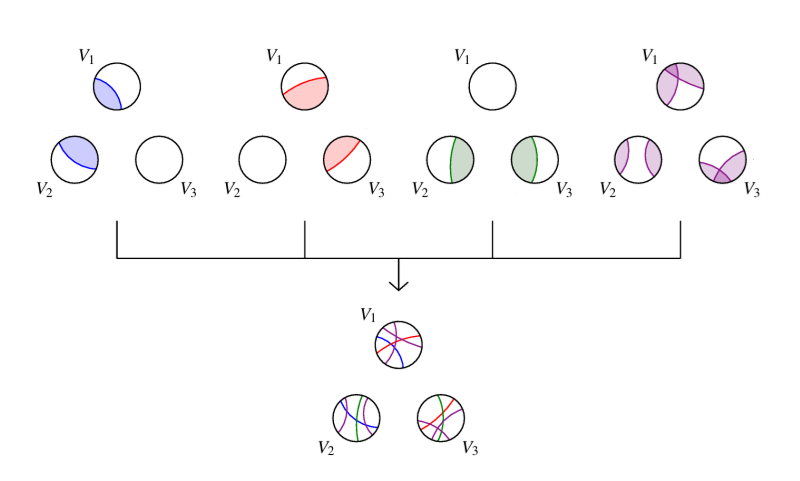
\includegraphics[width=0.8\textwidth]{Imágenes/Partition_by_irregularity.png}
        \caption[Ilustración del procedimiento de refinamiento simultáneo]{Ejemplo del refinamiento simultáneo por todos los subconjuntos que evidencian la irregularidad usando tres conjuntos de vértices (\cite{zhao2023graph}, página 59).}
        \label{refinamiento_irregularidad}
    \end{figure}

    Para simplicidad en la notación, se define $\Theta := \lbrace (i,j)\in [k]^{2} : (V_i,V_j)\ \text{es}\ \varepsilon\text{-regular}\rbrace$. Luego, como la partición $\mathcal{P}$ no es $\varepsilon$-regular, se cumple la desigualdad
    \begin{equation} \label{condición partición no regular}
        \sum_{(i,j)\not\in \Theta} \frac{|V_i||V_j|}{n^{2}} > \varepsilon.
    \end{equation}
    Así, junto a los lemas probados previamente, se da prueba al resultado de la siguiente manera:
    \begin{align*}
        q(\mathcal{Q}) &= \sum_{(i,j)\in [k]^{2}} q(\mathcal{Q}_i, \mathcal{Q}_j) \\
        &= \sum_{(i,j)\in \Theta} q(\mathcal{Q}_i, \mathcal{Q}_j) + \sum_{(i,j)\not\in \Theta} q(\mathcal{Q}_i, \mathcal{Q}_j)\\
        &\overset{\text{Lema \ref{energia_no_decrece}}}{\geq} \sum_{(i,j)\in \Theta} q(V_i, V_j) + \sum_{(i,j)\not\in \Theta} q(\lbrace A^{ij}, V_i\setminus A^{ij}\rbrace, \lbrace A^{ji}, V_{j}\setminus A^{ji}\rbrace)\\
        &\overset{\text{Lema \ref{Energy boost un conjunto}}}{\geq} \sum_{(i,j)\in \Theta} q(V_i, V_j) + \sum_{(i,j)\not\in \Theta} \left( q(V_i, V_j) + \varepsilon^{4}\frac{|V_i||V_j|}{n^{2}} \right)\\
        &= \sum_{(i,j)\in [k]^{2}} q(V_i, V_j) + \sum_{(i,j)\not\in \Theta} \varepsilon^{4}\frac{|V_i||V_j|}{n^{2}}\\
        &\overset{\eqref{condición partición no regular}}{\geq} q(\mathcal{P}) + \varepsilon^{5}.
    \end{align*}
\end{proof}
Este último lema culmina lo que se necesita para dar prueba formal del Lema de regularidad de Szemerédi mediante el argumento de incremento de energía.
\begin{proof}[Demostración del Teorema~\ref{szemeredi_regularity_lemma1}]
    Dado $\varepsilon > 0$ y un grafo $G$, elegimos inicialmente la partición trivial del conjunto de vértices $\mathcal{P} = \lbrace V(G)\rbrace$. Ahora, iterativamente (actualizando $\mathcal{P}$), aplicaremos el Lema~\ref{Energy boost particiones} cada vez que la partición actual no sea $\varepsilon$-regular. Observe que por cada aplicación del Lema~\ref{Energy boost particiones} se consigue un aumento de al menos $\varepsilon^{5}$ en la energía, y como la energía de toda partición está acotada superiormente por 1, el proceso iterativo terminará luego de a lo más $\varepsilon^{-5}$ pasos. El resultado será necesariamente una partición $\varepsilon$-regular debido a la cota de la energía. 

    Para una partición no $\varepsilon$-regular con $k$ elementos, el Lema~\ref{Energy boost particiones} encuentra un refinamiento de a lo más $k2^{k}$ partes. Dicho refinamiento será producido en cada iteración del algoritmo de \emph{argumento de incremento de energía}, y la cantidad de partes producidas las acotaremos crudamente en cada paso por $k2^{k} < 2^{2^{k}}$. Comenzando con la partición trivial de una parte, ejemplificaremos con las tres primeras iteraciones del algoritmo para mostrar la cantidad de partes producidas en cada paso tras aplicar el Lema~\ref{Energy boost particiones}.
    \begin{equation*}
        \begin{aligned}
            1^{\text{\underline{ra}}}\ \text{Iteración:}\quad & 1 & \to\quad & 2 < 2^{2} & \text{partes.}\\
            2^{\text{\underline{da}}}\ \text{Iteración:}\quad & 2^{2} & \to\quad & \left( 2^{2}\right)2^{\left(  2^{2}\right)}  <  2^{2^{2^{2}}} & \text{partes.}\\
            3^{\text{\underline{ra}}}\ \text{Iteración:}\quad & 2^{2^{2^{2}}} & \to\quad & \left( 2^{2^{2^{2}}} \right)2^{\left( 2^{2^{2^{2}}} \right)} < 2^{2^{2^{2^{2^{2}}}}} & \text{partes.}
        \end{aligned}
    \end{equation*}
    Finalmente, como el algoritmo debe terminar luego de a lo más $\varepsilon^{-5}$ iteraciones, la cantidad de partes al final del proceso será
    \begin{equation*}
        M(\varepsilon) \leq \left. 2^{2^{\cdot^{\cdot^{\cdot^{2}}}}}\right\rbrace\ \text{Altura }2\varepsilon^{-5}.
    \end{equation*}
\end{proof}
Desde ahora en adelante, vamos a definir y considerar una \emph{torre de altura $k$} de la siguiente manera:
\begin{equation*}
    \mathrm{torre}(k) := \left.2^{2^{\cdot^{\cdot^{\cdot^{2}}}}}\right\rbrace \text{Altura } k.
\end{equation*}
Durante la demostración del Teorema~\ref{szemeredi_regularity_lemma1} se utilizó una cota que podría parecer exagerada para encontrar la cantidad de partes que devuelve el algoritmo implementado, por sobre todo, considerando lo rápido que crece a medida que $\varepsilon$ se hace más pequeño. Sorprendentemente, en 1997, T. Gowers \cite{gowers1997lower} prueba que tal límite inferior de partes es necesario. Más precisamente, mostró que es posible encontrar una constante $c > 0$ tal que para todo suficientemente pequeño $\varepsilon > 0$, existe un grafo sin partición $\varepsilon$-regular siempre que posea una cantidad menor que $\mathrm{torre}(\lceil\varepsilon^{-c}\rceil)$ partes (ver G. Moshkovitz y A. Shapira \cite{moshkovitz2016short} para una demostración corta). 

Finalmente, se expone la forma de probar el Teorema~\ref{szemeredi_regularity_lemma2}. La idea de la demostración consiste en modificar el algoritmo de la técnica de argumento de incremento de energía, de manera que en cada iteración del refinamiento se logre obtener una equipartición. Este procedimiento conservará el incremento de energía en cada paso y  terminará con una equipartición del conjunto de vértices de un grafo cualquiera. Entonces, para todo grafo $G$, la modificación del algoritmo es la siguiente:
\begin{enumerate}
    \item Comenzar con una equipartición inicial arbitraria $\mathcal{P}$ de $V(G)$ con $m_0$ partes.
    \item Mientras la partición actual $\mathcal{P}$ no es $\varepsilon$-regular:
    \begin{itemize}
        \item[(a)] Para cada par $(V_i, V_j)$ no $\varepsilon$-regular, encontrar los subconjuntos $A^{ij}\subset V_i$ y  $A^{ji}\subset V_j$ que evidencian la irregularidad de los pares.
        \item[(b)] \label{paso_2b_mod} Refinar $\mathcal{P}$ usando simultáneamente los conjuntos $A^{ij}$ y $A^{ji}$ para obtener la partición $\mathcal{Q}$, cual divide cada parte de $\mathcal{P}$ en a lo más $2^{|\mathcal{P}|}$ partes.
        \item[(c)] \label{paso_3c_mod} Modificar la partición $\mathcal{Q}$ refinando, si es posible, cada uno de sus elementos para formar partes iguales de tamaño $|V(G)|/m$, dada alguna elección apropiada del entero $m=m(|Q|,\varepsilon)$. Luego, los elementos de $\mathcal{Q}$ que no fueron refinados previamente a causa de su bajo tamaño y los conjuntos de vértices residuales del refinamiento anterior, deben ser combinados y posteriormente dividir el resultado en partes iguales de tamaño $|V(G)|/m$.
        \item[(d)] Actualizar $\mathcal{P}$ con la modificación de $\mathcal{Q}$. 
    \end{itemize}
\end{enumerate}
El algoritmo anterior obtiene una equipartición del conjunto de vértices del grafo $G$. En lo que respecta a la energía del proceso, el paso~\ref{paso_2b_mod}(b) conserva un aumento de al menos $\varepsilon^{5}$ en cada iteración. El paso~\ref{paso_3c_mod}(c) podría ocasionar una baja en la energía, sin embargo, no debería ser significativa con una elección de $m$ suficientemente grande. En resumidas cuentas, el proceso anterior aumenta la energía en cada iteración en al menos $\varepsilon^{5}/2$, logrando terminar luego de a lo más $2\varepsilon^{-5}$ pasos con una equipartición de a lo más $\mathrm{torre}(\lceil\varepsilon^{-5}\rceil)$ partes.

\section{Demostración espectral} \label{Demo_esp}

En esta sección presentamos la demostración espectral del Lema de regularidad de Szemerédi. Originalmente, la prueba proviene de los autores A. Frieze y R. Kannan~\cite{frieze1996regularity}, y fue popularizada por T. Tao~\cite{taospectralproof2012}. Nuestra demostración se basa de la versión de T. Tao~\cite{taospectralproof2012} (ver también~\cite{cioabatao}).

%En 2012, T. Tao \cite{taospectralproof2012} publica en su blog una prueba del Lema de %regularidad de Szemerédi usando la descomposición espectral de la matriz de adyacencia. %La idea original de la demostración proviene de los autores A. Frieze y R. Kannan \cite%{frieze1996regularity}, a quienes Tao les da el crédito en su publicación. Más %adelante, en 2013, S. Cioba y R. Martin \cite{cioabatao} escribieron la demostración %con más detalles. La prueba que se expone en esta sección está basada esencialmente en %la publicación de Cioba y Martin.
%%%% Demostración espectral.
\begin{proof}[Demostración espectral del Teorema~\ref{szemeredi_regularity_lemma1}]
    Dado $\varepsilon > 0$, consideramos la función\newline $h:\mathbb{N}~\to\mathbb{N}$ definida por
    \begin{equation*}
        h(\ell) = \left\lceil\frac{1}{\varepsilon^{6}}\left( \frac{2\ell^{2}}{\varepsilon^{2}}\right)^{4\ell}\right\rceil.
    \end{equation*}
    Denotaremos por $h^{(i)}$ a la $i$-ésima composición de $h$ con ella misma, y escogemos $n_0\in\mathbb{N}$ suficientemente grande.

    Sea $G = ([n], E)$ un grafo con $n\geq n_0$ vértices, y $A$ su matriz de adyacencia. Ordenamos los valores propios $|\lambda_1|\geq ...\geq |\lambda_n|$ de $A$ de manera decreciente y consideramos $\boldsymbol{u}_1,...\boldsymbol{u}_n$ los vectores propios correspondientes, que forman una base ortonormal de $\mathbb{R}^{n}$.

    Por la Proposición~\ref{potencia_matriz_adyacencia = caminatas} y el Corolario~\ref{Tr_Ak}, se satisface
    \begin{equation} \label{eq_1 Spectral_Proof}
        \Tr(A^{2}) = \sum_{i=1}^{n} \lambda_{1}^{2} =  2e_G \leq n^{2}.
    \end{equation}
    De lo anterior, al notar que $i\lambda_{i}^{2} \leq \sum_{j=1}^{i} \lambda_{j}^{2} \leq n^{2}$, se encuentra la cota
    \begin{equation} \label{eq_2 Spectral_Proof}
        \lambda_{i} \leq \frac{n}{\sqrt{i}}\ ,\ \forall i\in [n].
    \end{equation}
    Consideramos también los intervalos $I_1,\dots, I_{\lceil1/\varepsilon^3\rceil}\subset [n]$ definidos por
    \begin{itemize}
        \item $I_1=\{1,2,\dots, h^{(1)}(1)-1\}$ y
        \item $I_k=\{h^{(k-1)}(1),\dots, h^{k}(1)-1\}$ para todo $k=2,\dots, I_{\lceil1/\varepsilon^3\rceil}$.
    \end{itemize}
    Con esta construcción, debe existir un natural $1\leq L \leq\lceil1/\varepsilon^3\rceil$ que cumple con
    \begin{equation} \label{eq_3 Spectral_Proof}
        \sum_{L \leq j < h(L)} \lambda_j^{2} \leq \varepsilon^{3}n^{2},
    \end{equation}
    porque de lo contrario, se obtiene
    \[\sum_{i=1}^n\lambda_i^2\geq \sum_{k=1}^{\lceil1/\varepsilon^3\rceil}\sum_{i\in I_k}\lambda_i^2> \lceil1/\varepsilon^3\rceil \cdot \varepsilon^3n^2>n^2,\]
    que contradice la desigualdad \eqref{eq_1 Spectral_Proof}.

    Ahora, usando $L$, separamos la matriz $A$ en tres matrices simétricas:
    \[        A= S + F + Q,\]
    donde la matriz $S$ se intepretará como la componente \emph{estructural},
    \begin{equation*}
        S = \sum_{i < L} \lambda_i \boldsymbol{u}_i \boldsymbol{u}_{i}^{T},
    \end{equation*}
    la matriz $F$ como la componente de \emph{error},
    \begin{equation*}
        F = \sum_{L \leq i < h(L)} \lambda_i \boldsymbol{u}_i \boldsymbol{u}_{i}^{T},
    \end{equation*}
    y la matriz $Q$ como la componente \emph{cuasi-aleatoria},
    \begin{equation*}
        Q = \sum_{i \geq h(L)} \lambda_i \boldsymbol{u}_i \boldsymbol{u}_{i}^{T}.
    \end{equation*}
    Usaremos los vectores propios $\boldsymbol{u}_1,...\boldsymbol{u}_{L-1}$ de $S$ para definir una partición de $V(G)$ como mostraremos a continuación. Consideramos el intervalo centrado en el origen de longitud $2\sqrt{({L}/{\varepsilon})}~\cdot n^{-1/2}$ de $\mathbb{R}$, y lo particionamos en $t = 2(L/\varepsilon)^{2}$ subintervalos $J_1,...,J_t$ de longitud $(\varepsilon /L)^{3/2}n^{-1/2}$ cada uno. Luego, clasificamos los vértices $v\in~V(G)$ según su valor $\boldsymbol{u}_i(v)$ de la siguiente manera:
    \[V^j_i=\big\{v\in V(G) :  \boldsymbol{u}_i(v)\in J_j\big\}\ ,\ 1\leq j\leq t.\]
    Tomamos el refinamiento de todos estos conjuntos $\big\{V_i^j\neq\emptyset : i\in[L-1], j\in[t]\big\}$ para obtener los conjuntos $V_0,V_1,...,V_M$, en donde $M\leq (\frac{2L^2}{\varepsilon^2})^L$. El resultado anterior considera un conjunto excepcional de vértices $V_0$ que está definido como sigue:
    \begin{equation*}
        V_{0} = \left\lbrace v\in  V(G): |\boldsymbol{u}_i (v)| > \sqrt{\frac{L}{\varepsilon}}n^{-1/2}\text{ para alg\'un }i\in[L-1]\right\rbrace .
    \end{equation*}
    Mostraremos que el conjunto excepcional $V_0$ es suficientemente pequeño. En efecto, observando que
    \begin{equation*}
        L-1= \sum_{i=1}^{L-1} \norm{\boldsymbol{u}_i}^{2} \geq  \sum_{i=1}^{L-1}\sum_{v\in V(G)}^{n} \boldsymbol{u}_{i}(v)^{2} \geq |V_{0}|\left( {\frac{L}{\varepsilon n}}\right),
    \end{equation*}
    se determina que $|V_0| < \varepsilon n$.

    Probaremos que la partición construida del conjunto de vértices del grafo\newline $\mathcal{P} =\lbrace V_0,V_1,...,V_M\rbrace$ es $\varepsilon$-regular. Comenzamos identificando los pares excepcionales. Para esto, sea $F = (f_{xy})$ indexando $(x,y)$ con $V_i \times V_j$, y defina
    \begin{align*}
        \Sigma_F &=\Big\{(i,j) : \sum_{(x,y)\in V_i\times V_j} f_{xy}^{2} > \varepsilon |V_i| |V_j|\Big\}.
    \end{align*}
    Entonces, por la simetría de $F$ se tiene que $\Tr(F^2)=  \sum_{x\in V(G)} \sum_{y\in V(G)}  f_{xy}^2$, y por lo tanto
    \begin{align*}
        \varepsilon^3n^2\geq \sum_{L\leq i<h(L)}\lambda_i^2 =\Tr(F^2)&=  \sum_{(x,y)\in V(G)^2} f_{xy}^2\\
        &\geq \sum_{(i,j)\in \Sigma_F}\sum_{(x,y)\in V_i\times V_j} f_{xy}^{2} > \varepsilon \sum_{(i,j)\in\Sigma_F} |V_i| |V_j|.
    \end{align*}
    Así,
    \begin{equation} \label{eq_8 Spectral_Proof}
        \varepsilon^{2} n^{2}\geq  \sum_{(i,j)\in \Sigma_F} |V_i| |V_j|.
    \end{equation}
    Además, sea
    \[\Sigma_Q=\Big\{(i,j) : \min\{|V_i|,|V_j|\}<\frac\varepsilon Mn\Big\} \cup \big\{(i,j) : i=0\lor j=0\big\},\]
    y observe que
    \[ \sum_{(i,j)\in \Sigma_Q} |V_i| |V_j|\leq 2M\cdot\frac\varepsilon M n+ 2|V_0|n<4\varepsilon n.\]
    Ahora, sea $(i,j)\not\in \Sigma_F\cup\Sigma_Q$, y $d_{ij}=d(V_i,V_j)$ la densidad del par $(V_i,V_j)$. Entonces, dado los subconjuntos $X\subset V_i$ e $Y\subset V_j$, note la siguiente descomposición:
    \begin{align} \label{tres_sumandos_demo_esp} 
        \Big| e(X,Y) - d_{ij}|X||Y|\Big|& =\Big|\boldsymbol{v}_X^T A\boldsymbol{v}_Y - d_{ij}|X||Y|\Big|\nonumber\\
        &\leq \Big|\boldsymbol{v}_X^T S\boldsymbol{v}_Y - d_{ij}|X||Y| \Big|+\Big|\boldsymbol{v}_X^T F\boldsymbol{v}_Y \Big|+\Big|\boldsymbol{v}_X^T Q\boldsymbol{v}_Y \Big|.
    \end{align}
    En este punto, el objetivo es encontrar cotas para cada uno de los sumandos anteriores.

    Para comenzar, por la definición de $\Sigma_F$ y la desigualdad de Cauchy-Schwarz, se obtiene la primera de las cotas de la siguiente manera:
    \begin{align} \label{cota_esp_1}
        \left| \boldsymbol{v}_{X}^{T} F \boldsymbol{v}_Y\right|^{2} = \Big| \sum_{(x,y)\in X\times Y} f_{xy}\Big|^{2} &\overset{\mathrm{DCS}}{\leq} \Big( \sum_{(x,y)\in X\times Y} f_{xy}^{2}\Big)|X||Y|\nonumber\\
        &\leq \varepsilon^{2} |V_i| |V_j| |X| |Y|
        \leq \varepsilon^{2} |V_i|^{2} |V_j|^{2}.
    \end{align}    
    Para la próxima cota, debemos observar por la construcción de $Q$ y el Teorema~\ref{Teo Courant-Fischer} que
    \begin{align*} 
        \left| \boldsymbol{v}_{X}^{T} Q \boldsymbol{v}_Y\right|   \overset{\mathrm{DCS}}{\leq} \norm{\boldsymbol{v}_X} \norm{Q \boldsymbol{v}_Y} \leq \norm{\boldsymbol{v}_X} \norm{\boldsymbol{v}_Y} \frac{n}{\sqrt{h(L)}}
        = \sqrt{|X| |Y|} \frac{n}{\sqrt{h(L)}}\leq \frac{n^{2}}{\sqrt{h(L)}}.
    \end{align*}
    Como $M\leq (\frac{2L^2}{\varepsilon^2})^L$, concluimos de la elección de $h(\cdot)$ que $h(L) \geq \frac{1}{\varepsilon^{6}}\left( \frac{2L^{2}}{\varepsilon^{2}}\right)^{4L}\geq  \frac{1}{\varepsilon^{6}} M^4$. Y así, cuando $(i,j)\not= \Sigma_Q$, se tiene
    \begin{align} \label{cota_esp_2}
        \left| \boldsymbol{v}_{X}^{T} Q \boldsymbol{v}_Y\right|\leq   \frac{n^{2}}{\sqrt{h(L)}} \leq  \frac{M^{2} |V_i| |V_j|}{\varepsilon^{2}\sqrt{h(L)}}\leq \varepsilon|V_i| |V_j|.
    \end{align}
    Por último, para la tercera cota, analizamos $S = (s_{xy})$. Sean $s_{ab}$ y $s_{cd}$ los valores mínimo y máximo de todos los $s_{xy}$ sobre $(u,v)\in V_{i}\times V_{j}$. Entonces,
    \begin{align*}
        s_{cd}-s_{ab}  &=  \sum_{i < L} \lambda_i \boldsymbol{u}_i(c) \boldsymbol{u}_i(d) - \lambda_i \boldsymbol{u}_i(a) \boldsymbol{u}_i(b)\\
        &\leq \sum_{i < L} \left| \lambda_i\right| \Big| \boldsymbol{u}_i(c) \boldsymbol{u}_i(d) - \boldsymbol{u}_i(a)\boldsymbol{u}_i(d) + \boldsymbol{u}_i(a)\boldsymbol{u}_i(d) - \boldsymbol{u}_i(a)\boldsymbol{u}_i(b)\Big|\\
        &\leq n\sum_{i < L}  \Big| \boldsymbol{u}_i(d)\big(\boldsymbol{u}_i(c) - \boldsymbol{u}_i(a)\big) + \boldsymbol{u}_i(a)\big(\boldsymbol{u}_i(d) - \boldsymbol{u}_i(b)\big)\big|\\
        &\leq n\sum_{i < L}  \left| \boldsymbol{u}_i(b)\right| \Big| \boldsymbol{u}_i(a) - \boldsymbol{u}_i(c)\Big| + \left| \boldsymbol{u}_i(c)\right| \Big| \boldsymbol{u}_i(b) - \boldsymbol{u}_i(d)\Big|\\
        &\leq L n\cdot 4\cdot \sqrt{\frac{L}{\varepsilon n}} \cdot \frac{\varepsilon}{L}\sqrt{\frac{\varepsilon}{L n}}\\
        &= 4\varepsilon.
    \end{align*}
    Ahora bien, como $d_{ij}$ es el promedio de $S$ sobre $V_{i}\times V_j$, tenemos que $s_{ab} \leq d_{ij} \leq s_{cd}$, y por ende, $|s_{xy}-d_{ij}| \leq s_{cd}-s_{ab}$ para cada $(u,v)\in V_i \times V_j$. Como resultado,
    \begin{align} \label{cota_esp_3}  
        \left| \boldsymbol{v}_{X}^{T}S\boldsymbol{v}_Y-d_{ij}|V_i||V_j|\right| &\leq \sum_{(x,y)\in X\times Y} \left| s_{xy} - d_{ij}\right|\leq (s_{cd}-s_{ab})|X||Y|\leq 4\varepsilon |X||Y|.
    \end{align}
    Utilizando las desigualdades~\eqref{cota_esp_1}, \eqref{cota_esp_2} y~\eqref{cota_esp_3} en la expresión enunciada en~\eqref{tres_sumandos_demo_esp} se concluye la demostración del teorema.
\end{proof}

\section{Aplicaciones} \label{Sec. Aplicaciones}

Usualmente las aplicaciones del Lema de regularidad de Szemerédi son abordadas con el \emph{método de regularidad} que se describe en los siguientes pasos:
\begin{enumerate}
    \item Obtener una \textbf{partición} del conjunto de vértices de un grafo con el Lema de regularidad.
    \item \textbf{Limpiar} las aristas del que tengan un ``mal comportamiento'' según el problema. Generalmente, se eliminan las aristas entre los pares de partes que presentan:
    \begin{itemize}
        \item[(i)] Irregularidad.
        \item[(ii)] Baja densidad.
        \item[(iii)] Al menos una de las partes demasiado pequeña.    
    \end{itemize}
    \item \textbf{Contar} un determinado patrón en el grafo limpio.
\end{enumerate} 
Para el último paso se utilizará un resultado análogo a la propiedad $\Count_{p}(\varepsilon)$ del Teorema~\ref{Teorema CGW}, pero con el concepto de par $\varepsilon$-regular. Las aplicaciones que se estudiarán en esta tesis solo necesitan el caso en que $H = K_3$, el cual es conocido como Lema de conteo de triángulos.
\begin{lema} \label{Triangle_Counting_Lemma} (Lema de conteo de triángulos)
    Sea $\varepsilon > 0$, $G = (V,E)$ un grafo, y los conjuntos no necesariamente disjuntos $X,Y,Z\subset V$ tales que los pares $(X,Y), (Y,Z)$ y $(X,Z)$ son $\varepsilon$-regular. Entonces,
    \begin{align*}
        \Big|\lbrace (x,y,z)\in X\times Y\times Z : xy,xz,yz\in E\rbrace\Big| &= d(X,Y)d(X,Z)d(Y,Z)|X||Y||Z|\\
        &\quad \pm 3\varepsilon |X||Y||Z|.
    \end{align*}
\end{lema}
\begin{proof} %%%% Demostración Teorema: Lema de conteo de triángulos
    Se realizará un proceso inductivo similar al visto en la demostración de la Proposición~\ref{discp => count} sobre la cantidad de aristas del grafo $K_3 = ([3], \lbrace 12, 23, 13\rbrace)$. Cuando el grafo no posee aristas, entonces
    \begin{equation*}
        \Big|\lbrace (x,y,z)\in X\times Y\times Z : xy,xz,yz\not\in E\rbrace\Big| = |X||Y||Z|.
    \end{equation*}
    También, como vimos en \eqref{BIDISC}, recordamos que la condición de un par $\varepsilon$-regular es equivalente a la propiedad $\disc_p (\varepsilon)$ en grafos bipartitos para algún $p\in(0,1)$. Entonces, cuando el grafo presenta solo una arista,
    \begin{equation*}
        \Big|\lbrace (x,y,z)\in X\times Y\times Z : xy\in E\rbrace\Big| = \left( d(X,Y)|X||Y| \pm \varepsilon|X||Y| \right)|Z|.
    \end{equation*}
    Ahora, se plantea la hipótesis inductiva de la siguiente manera:
    \begin{equation*}
        \Big|\lbrace (x,y,z)\in X,Y,Z : xy,yz\in E\rbrace\Big| = d(X,Y)d(Y,Z)|X||Y||Z| \pm 2\varepsilon |X||Y||Z|.
    \end{equation*}
    Sea $T^{-}$ el grafo correspondido a una copia etiquetada del grafo $([3],\lbrace 12,23\rbrace)$ en $G$ bajo la apliación inyectiva $\varphi : [3]\to V(T^{-})\subset V$. Con esto, defina $e^{-} = \varphi(1)\varphi(3)$ y se desarrolla inductivamente como sigue:
    \begin{align} \label{2doSum_TCL}
        \Big|&\lbrace (x,y,z)\in X\times Y\times Z : xy,yz,xz\in E\rbrace\Big| = \sum_{T^{-}} \left[ \mathbbm{1}_{E}(e^{-}) + d(X,Z) - d(X,Z) \right]\nonumber \\
        &= d(X,Y)d(Y,Z)d(X,Z)|X||Y||Z| + \sum_{T^{-}} \left( \mathbbm{1}_{E}(e^{-}) - d(X,Z)\right) \pm 2\varepsilon |X||Y||Z|.
    \end{align}
    En este punto, nos falta probar que el segundo sumando de la igualdad \eqref{2doSum_TCL} se corresponde con un factor de error, para esto, sea $T^{*}$ una copia del grafo singleton $\lbrace 2\rbrace$ en $G$, y considere los siguientes conjuntos:
    \[
        A_{1}^{T^{*}} = \lbrace x\in X: T^{*} \text{ con } x \text{ forma una copia de } (\lbrace 1,2\rbrace, \lbrace 12\rbrace) \text{ en } G\rbrace.
    \]
    \[
        A_{3}^{T^{*}} = \lbrace z\in Z: T^{*} \text{ con } z \text{ forma una copia de } (\lbrace 2,3\rbrace, \lbrace 23\rbrace) \text{ en } G\rbrace.
    \]
    De esta manera, dada la equivalencia de la condición del par $(X,Z)$ $\varepsilon$-regular con versión bipartita de la propiedad $\disc_{d(X,Z)}(\varepsilon)$ vista en \eqref{BIDISC}, se consigue la siguiente desigualdad:
    \begin{align*}
        \left| \sum_{T^{-}} \left( \mathbbm{1}_{E}(e^{-})\right) - d(X,Z)\right| &\leq \sum_{T^{*}} \left| \sum_{f\in A_{1}^{T^{*}}\times A_{3}^{T^{*}}} \left( \mathbbm{1}_{E}(f) - d(X,Z)\right)\right|\\
        &= \sum_{T^{*}} \left| e(A_{1}^{T^{*}}, A_{3}^{T^{*}}) - d(X,Z)|A_{1}^{T^{*}}||A_{3}^{T^{*}}|\right|\\
        &\leq \sum_{T^{*}} \varepsilon |X||Z|\\
        &\leq \varepsilon |X||Y||Z|.
    \end{align*}
    Finalmente, aplicando la última desigualdad en la ecuación \eqref{2doSum_TCL} se prueba lo prometido.
\end{proof}
En la demostración anterior solo fue necesario utilizar que los pares $(X,Y)$ y $(X,Z)$ son $\varepsilon$-regular, por lo que es interesante destacar que uno de los pares de conjuntos de vértices podría no ser necesariamente un par $\varepsilon$-regular para que el Lema de conteo de triángulos funcione correctamente.

Bajo el mismo planteamiento de la inducción vista en la demostración del Lema~\ref{Triangle_Counting_Lemma} (y Proposición~\ref{discp => count}), es posible generalizar el resultado para contar apropiadamente cualquier grafo $H$. Se enuncia sin demostración.
\begin{lema} \label{Lema_Conteo_Grafos} (Lema de conteo de grafos)
    Sea $\varepsilon > 0$, $H$ un grafo sobre $k$ vértices, y $G$ un grafo de $n$ vértices con los subconjuntos disjuntos $V_1 ,..., V_k\subset V(G)$ tales que los pares $(V_i, V_j)$ son $\varepsilon$-regular siempre que $ij\in E(H)$. Entonces, la cantidad de tuplas $(v_1,...,v_k)\in V_1\times\cdots\times V_k$ tales que $v_i v_j\in E(G)$ cada vez que $ij\in E(H)$ es
    \begin{equation*}
        \left( \prod_{ij\in E(H)} d(V_i, V_j)\right) \left( \prod_{\ell=1}^{k}|V_{\ell}|\right) \pm e_H\cdot \varepsilon \prod_{\ell = 1}^{k}|V_{\ell}|.
    \end{equation*}
\end{lema}
En las siguientes subsecciones se discutirán dos aplicaciones del método de regularidad para entregar dos demostraciones alternativas al Teorema de Roth.

\subsection{Eliminación de triángulos}

El Lema de eliminación de triángulos fue probado por los autores I. Ruzsa y E. Szemerédi \cite{ruzsa1978triple} en 1976, y es una de las primeras aplicaciones del método de regularidad. La intuición del lema dice que todo grafo con \emph{pocos} triángulos se puede convertir en un grafo libre de triángulos eliminando \emph{pocas} aristas. Formalmente,
\begin{teorema} \label{Enunciado TRL} (Lema de eliminación de triángulos)
    Para todo $\varepsilon > 0$, existe $\delta > 0$ y $n_0\in \mathbb{N}$ tal que todo grafo sobre $n\geq n_0$ vértices con a lo más $\delta n^{3}$ triángulos se puede hacer libre de triángulos eliminando a lo más $\varepsilon n^{2}$ aristas.
\end{teorema}
\begin{proof} %%%% Demostración Teorema: Lema de eliminación de triángulos
    Dado $\varepsilon > 0$, elija $\varepsilon_r = \frac{1}{4}\left(  \frac{\varepsilon}{3}\right)^{3}$ y  utilice el Teorema~\ref{szemeredi_regularity_lemma1} con tal elección para obtener la constante $M=M(\varepsilon_r)$. Considere además $\delta = \frac{1}{2}\frac{\varepsilon_{r}^{4}}{M^{3}}$ y $n_0\in\mathbb{N}$ suficientemente grande, de manera tal que el grafo $G = (V,E)$ con $n\geq n_0$ vértices posee a lo más $\delta n^{3}$ triángulos. Luego, nuevamente por el Teorema~\ref{szemeredi_regularity_lemma1}, se asegura la existencia de una partición $\varepsilon_r$-regular $\mathcal{P} = \lbrace V_1,...,V_k \rbrace$, con $k \leq M$.

    Para limpiar el grafo, para cada $(i,j)\in [k]^{2}$, se eliminan todas las aristas entre $V_i$ y $V_j$ cuando
    \begin{itemize}
        \item[(a)] ($V_i , V_j$) no es un par $\varepsilon_r$-regular,
        \item[(b)] $d(V_i, V_j) < (4\varepsilon_r)^{1/3}$, o
        \item[(c)] $\min\lbrace |V_i||V_j|\rbrace < \frac{n}{k}\varepsilon_r$.
    \end{itemize}
    De esta manera, como la partición es $\varepsilon_r$-regular, las aristas removidas por la condición (a) son a lo más
    \begin{equation*}
        \sum_{\substack{(i,j)\in [k]^{2} \\ (V_i , V_j) \text{ no } \varepsilon_r\text{-regular}}} |V_i||V_j|\leq \varepsilon_r n^{2}.
    \end{equation*}
    Las aristas eliminadas en los conjuntos de baja densidad por la condición (b) son a lo más
    \begin{equation*}
        \sum_{\substack{(i,j)\in [k]^{2} \\ d(V_i, V_j) < (4\varepsilon_r)^{1/3}}} d(V_i, V_j)|V_i||V_j| < (4\varepsilon_r)^{1/3} \sum_{(i,j)\in [k]^{2}} |V_i||V_j| = (4\varepsilon_r)^{1/3} n^{2}.
    \end{equation*}
    Por último, debido a que cada vértice de $G$ puede ser adyacente con a lo más $\frac{n}{k}\varepsilon_r$ vértices en a lo más $k$ subconjuntos demasiado pequeños, las aristas removidas por (c) son a lo más
    \begin{equation*}
        k\cdot \frac{n}{k}\varepsilon_r \cdot n = \varepsilon_r n^{2}.
    \end{equation*}
    En total, en la limpieza, se eliminan a lo más $\varepsilon n^{2}$ aristas.

    Ahora, nos falta probar que el grafo limpio $G' = (V, E')$ es libre de triángulos. Para esto, con nuestra elección de $\delta$, buscaremos formular la siguiente contradicción: si existe un triángulo en el grafo limpio $G'$, el Lema de conteo de triángulos asegura que en realidad existen más de $\delta n^{3}$ triángulos. No obstante, como el grafo original posee a lo más $\delta n^{3}$ triángulos, se podrá concluir que el grafo $G'$ es libre de triángulos eliminando a lo más $\varepsilon n^{2}$ aristas.

    Dicho esto, estudiamos la cantidad de triángulos en $G'$. Dada la eliminación de aristas según la condición (a), cada par $(V_i , V_j)$ es $\varepsilon$-regular, y por ende se satisface la hipótesis del Lema~\ref{Triangle_Counting_Lemma}. Entonces, gracias a la ausencia de las aristas que cumplían con las condiciones (b) y (c),
    \begin{align*}
        \left| \lbrace (x,y,z)\in V_i\times V_j\times V_\ell : xy,yz,xz\in& E'\rbrace\right| \geq d(V_i, V_j)d(V_i, V_\ell)d(V_j, V_\ell)|V_i||V_j||V_\ell| \\
        &\quad - 3\varepsilon_r |V_i||V_j||V_\ell| \\
        &\geq \varepsilon_r |V_i| |V_j| |V_\ell| \\
        &\geq \frac{\varepsilon^{4} n^{3}}{k^{3}} \\
        &> \delta n^{3}.
    \end{align*}
    Así, de la contradicción anterior, se determina que el grafo $G$ es libre de triángulos eliminando a lo más $\varepsilon n^{2}$ aristas.
\end{proof}
Otra forma de entender el Teorema~\ref{Enunciado TRL} es de la siguiente manera: si se necesitan eliminar al menos $\varepsilon n^{2}$ para hacer de $G$ libre de trángulos, entonces $G$ contiene al menos $\delta n^{3}$ triángulos.

\subsection{Emparejamiento inducido}

Dado un grafo $G = (V,E)$, un subconjunto $R\subset E$ es un \textbf{emparejamiento} en $G$ si no existe un par de aristas en $R$ que compartan algún vértice. Diremos que $R$ es un \textbf{emparejamiento inducido} si es un emparejamiento y no existen un par de aristas en $R$ que estén conectadas por una arista de $G$, es decir, no existen aristas en $G$ entre cada par de vértices de $R$.
%%%% Ejemplo emparejamientos
\begin{figure}[h]
    \centering
    \begin{tikzpicture}
        %% Grafo original, G
        \node at (-5, -2) {\small Grafo original $G$};
        % Vértices
        \node[fill=black, circle, inner sep=2pt, minimum size=4pt] (1_l1) at (-6.5, 1.5) {};
        \node[fill=black, circle, inner sep=2pt, minimum size=4pt] (1_l2) at (-6.5, 0.5) {};
        \node[fill=black, circle, inner sep=2pt, minimum size=4pt] (1_l3) at (-6.5, -0.5) {};
        \node[fill=black, circle, inner sep=2pt, minimum size=4pt] (1_l4) at (-6.5, -1.5) {};
        \node[fill=black, circle, inner sep=2pt, minimum size=4pt] (1_r1) at (-3.5, 1.5) {};
        \node[fill=black, circle, inner sep=2pt, minimum size=4pt] (1_r2) at (-3.5, 0.5) {};
        \node[fill=black, circle, inner sep=2pt, minimum size=4pt] (1_r3) at (-3.5, -0.5) {};
        \node[fill=black, circle, inner sep=2pt, minimum size=4pt] (1_r4) at (-3.5, -1.5) {};
        % Aristas
        \draw[line width=1.2pt] (1_l1) -- (1_r1);
        \draw[line width=1.2pt] (1_l1) -- (1_r3);
        \draw[line width=1.2pt] (1_l2) -- (1_r1);
        \draw[line width=1.2pt] (1_l2) -- (1_r4);
        \draw[line width=1.2pt] (1_l3) -- (1_r2);
        \draw[line width=1.2pt] (1_l3) -- (1_r4);
        \draw[line width=1.2pt] (1_l4) -- (1_r1);
        \draw[line width=1.2pt] (1_l4) -- (1_r2);

        %% Emaparejamiento en G
        \node at (0, -2) {\small Emparejamiento en $G$};
        % Vértices
        \node[fill=black, circle, inner sep=2pt, minimum size=4pt] (2_l1) at (-1.5, 1.5) {};
        \node[fill=black, circle, inner sep=2pt, minimum size=4pt] (2_l2) at (-1.5, 0.5) {};
        \node[fill=black, circle, inner sep=2pt, minimum size=4pt] (2_l3) at (-1.5, -0.5) {};
        \node[fill=black, circle, inner sep=2pt, minimum size=4pt] (2_l4) at (-1.5, -1.5) {};
        \node[fill=black, circle, inner sep=2pt, minimum size=4pt] (2_r1) at (1.5, 1.5) {};
        \node[fill=black, circle, inner sep=2pt, minimum size=4pt] (2_r2) at (1.5, 0.5) {};
        \node[fill=black, circle, inner sep=2pt, minimum size=4pt] (2_r3) at (1.5, -0.5) {};
        \node[fill=black, circle, inner sep=2pt, minimum size=4pt] (2_r4) at (1.5, -1.5) {};
        % Aristas
        \draw[line width=1.2pt] (2_l1) -- (2_r1);
        \draw[line width=1.2pt, red!70!black] (2_l1) -- (2_r3);
        \draw[line width=1.2pt, red!70!black] (2_l2) -- (2_r1);
        \draw[line width=1.2pt] (2_l2) -- (2_r4);
        \draw[line width=1.2pt] (2_l3) -- (2_r2);
        \draw[line width=1.2pt, red!70!black] (2_l3) -- (2_r4);
        \draw[line width=1.2pt] (2_l4) -- (2_r1);
        \draw[line width=1.2pt, red!70!black] (2_l4) -- (2_r2);

        %% Emparejamiento inducido
        \node at (5,-2) {\small Emparejamiento inducido en $G$};
        % Vértices
        \node[fill=black, circle, inner sep=2pt, minimum size=4pt] (3_l1) at (3.5, 1.5) {};
        \node[fill=black, circle, inner sep=2pt, minimum size=4pt] (3_l2) at (3.5, 0.5) {};
        \node[fill=black, circle, inner sep=2pt, minimum size=4pt] (3_l3) at (3.5, -0.5) {};
        \node[fill=black, circle, inner sep=2pt, minimum size=4pt] (3_l4) at (3.5, -1.5) {};
        \node[fill=black, circle, inner sep=2pt, minimum size=4pt] (3_r1) at (6.5, 1.5) {};
        \node[fill=black, circle, inner sep=2pt, minimum size=4pt] (3_r2) at (6.5, 0.5) {};
        \node[fill=black, circle, inner sep=2pt, minimum size=4pt] (3_r3) at (6.5, -0.5) {};
        \node[fill=black, circle, inner sep=2pt, minimum size=4pt] (3_r4) at (6.5, -1.5) {};
        % Aristas
        \draw[line width=1.2pt] (3_l1) -- (3_r1);
        \draw[line width=1.2pt, red!70!black] (3_l1) -- (3_r3);
        \draw[line width=1.2pt] (3_l2) -- (3_r1);
        \draw[line width=1.2pt, red!70!black] (3_l2) -- (3_r4);
        \draw[line width=1.2pt] (3_l3) -- (3_r2);
        \draw[line width=1.2pt] (3_l3) -- (3_r4);
        \draw[line width=1.2pt] (3_l4) -- (3_r1);
        \draw[line width=1.2pt, red!70!black] (3_l4) -- (3_r2);
    \end{tikzpicture}
    \caption[Ejemplo de un emparejamiento y un emparejamiento inducido]{Ejemplo de un emparejamiento y un emparejamiento inducido.}
\end{figure}

La presente aplicación del método de regularidad responde a la pregunta: \emph{¿Cuántas aristas puede tener un grafo que es la unión de emparejamientos inducidos?}.
\begin{teorema}  \label{Teo_emp_ind} (Emparejamiento inducido)
    Para todo $\varepsilon > 0$, existe $n_0\in \mathbb{N}$ tal que todo grafo $G = (V,E)$ de $n\geq n_0$ vértices que está compuesto por la unión de $n$ emparejamientos inducidos, posee a lo más $\varepsilon n^{2}$ aristas.
\end{teorema}
\begin{proof} %%%% Demostración: Emparejamiento inducido
    Dado $\varepsilon > 0$, aplique el Teorema~\ref{szemeredi_regularity_lemma1} con $\varepsilon_r = \frac{\varepsilon}{10}$ para obtener la constante $M(\varepsilon_r)$. Considere $n_0\in\mathbb{N}$ suficientemente grande, y asuma que el grafo $G = (V,E)$ con $n\geq n_0$ vértices y compuesto por $n$ emparejamientos inducidos satisface $e_G > \varepsilon n^{2}$. Nuevamente, por el Teorema~\ref{szemeredi_regularity_lemma1}, se asegura la existencia de la partición $\mathcal{P} = \lbrace V_1,...,V_k\rbrace$ con $k\leq M(\varepsilon)$ partes que es $\varepsilon_r$-regular.
    
    Para cada $(i,j)\in [k]^{2}$ se eliminan todas las aristas entre los conjuntos $V_i$ y $V_j$ cuando estos presenten irregularidad, densidad menor que $2\varepsilon_r$, o al menos uno de los conjuntos es menor que $\frac{n}{k}\varepsilon_r$. En total, el proceso de limpieza remueve a lo más $4\varepsilon_r n^{2}$ aristas de $G$ para obtener un nuevo grafo $G'$. En consecuencia,
    \begin{equation*}
        e_G' \geq e_G - 4\varepsilon_r n^{2} > \varepsilon n^{2} - \frac{4}{10}\varepsilon n^{2} > \frac{\varepsilon}{2}n^{2}.
    \end{equation*}
    Ahora, observe que debe existir un emparejamiento inducido $R$ en $G'$ con al menos $\frac{\varepsilon}{2}n$ aristas (y al menos $\varepsilon n$ vértices). De no ser así, todos los emparejamientos tendrán a lo más $\frac{\varepsilon}{2}n$ aristas, por lo que $e_G' < \frac{\varepsilon}{2}n^{2}$.

    Denotando por $V(R)$ al conjunto de vértices que componen las aristas de $R$, se define $U_i := V_i \cap V(R)$ como el subconjunto de vértices de $R$ que comparte elementos con $V_i$, y $U := \displaystyle\bigcup_{i\in [k]} \lbrace U_i : |U_i| \geq \varepsilon_r |V_i|\rbrace$. Es decir, $U$ es la unión de todos los conjuntos $U_i \subset V(R)$ que comparten una fracción suficientemente grande de vértices con $V_i$. Note que podemos obtener el conjunto $U$ removiendo a lo más $\varepsilon_r n = \frac{\varepsilon}{10}n$ vértices de $V(R)$, pues
    \begin{equation*}
        \sum_{i\in [k]} |U_i| < \sum_{i\in [k]} \varepsilon_r |V_i| = \frac{\varepsilon}{10} n.
    \end{equation*}
    Luego, recordando que $|V(R)| \geq \varepsilon n$, se determina que $|U| > \varepsilon n - \frac{\varepsilon}{10}n = \frac{9}{10}\varepsilon n$. Además, como también $|R| \geq \frac{\varepsilon}{2}n$, debe existir al menos un vértice en $U$ que sea parte de una arista en $R$. Luego, dada la limpieza de $G$, dicha arista debe pertenecer a algún par $U_t\times U_\ell$ que satisfacen $|U_k| \geq \varepsilon_r |V_k|$ y  $|U_\ell| \geq \varepsilon_r |V_\ell|$, y son tales que 
    su correspondiente par $(V_t, V_\ell)$ es $\varepsilon_r$-regular con densidad $d(V_t, V_\ell) \geq 2\varepsilon_r$. Entonces, por regularidad,
    \begin{equation} \label{eq1_emp_ind}
        d(U_t, U_\ell) = d(V_t, V_\ell) \pm \varepsilon_r \geq 2\varepsilon_r - \varepsilon_r = \varepsilon_r.
    \end{equation}
    Así, como $R$ es un emparejamiento inducido, todo par de subconjuntos $A,B\subset V(M)$ debe satisfacer
    \begin{equation*}
        e(A,B) \leq \min\lbrace |A|, |B|\rbrace.
    \end{equation*}
    Sin embargo, la desigualdad \eqref{eq1_emp_ind} implica que
    \begin{align*}
        e(U_t, U_\ell) &= d(U_t, U_\ell)|U_t||U_\ell|\\
        &\geq |U_t||U_\ell| \varepsilon_r\\
        &\geq |U_t| |V_\ell| \varepsilon_{r}^{2}\\
        &\geq |U_t|\frac{n}{k}\varepsilon_{r}^{3}\\
        &> |U_t|.
    \end{align*}
    La desigualdad anterior nos dice que existe una arista entre $U_k$ y $U_\ell$ que no pertenece a $R$, por lo que se contradice la hipótesis de que $R$ es un emparejamiento inducido. 
\end{proof}
Otra mirada del Teorema~\ref{Teo_emp_ind} es la siguiente: si $G$ posee al menos $\varepsilon n^{2}$ aristas, entonces $G$ tiene al menos un emparejamiento no inducido.

\subsection{Teorema de Roth}

Como hemos visto en el comienzo de la sección~\ref{Sec. LRS}, el Teorema de Roth es un caso particular del Teorema de Szemerédi, el cual en un principio fue demostrado utilizando análisis de Fourier. 
\begin{teorema} (Teorema de Roth) \label{Teorema_de_Roth}
    Para todo $\varepsilon > 0$, existe $n_0 \in \mathbb{N}$ tal que si el conjunto $S\subset [n]$ posee $|S| \geq \varepsilon n$ elementos, entonces $S$ contiene una progresión aritmética no trivial de largo $3$.
\end{teorema}
En esta sección se entregarán dos demostraciones del Teorema de Roth por medio del Lema de regularidad de Szemerédi. Como el enunciado del Teorema~\ref{Teorema_de_Roth} alude a la teoría de números, en ambas pruebas, la idea es traducir el problema al lenguaje de la teoría de grafos con la construcción de un grafo apropiado. La primera demostración se fundamenta en el Lema de eliminación de triángulos.
\begin{proof}[Primera demostración del Teorema \ref{Teorema_de_Roth}]
    Considerando $\varepsilon > 0$, utilizamos el Teorema~\ref{Enunciado TRL} con $\frac{\varepsilon}{36}$ para recibir $\delta > 0$. Sea $S\subset [n]$ con $|S|\geq \varepsilon n$ elementos, y escogemos $n_0\in\mathbb{N}$ suficientemente grande.
    
    Una manera natural de construir un grafo de $n$ vértices utilizando el conjunto $S$, es definir una arista entre los vértices $i$ y $j$ si y solamente si $|i-j|\in S$. Sin embargo, con $n$ elementos no podemos describir una progresión aritmética de largo $3$ por medio de relaciones entre las aristas. Por esto, agregamos un poco de asimetría a la construcción. Para asegurar que las sumas siempre tengan la posibilidad de estar en $S$, consideramos el grafo $3$-partito $G=(V,E)$ con partición de vértices $V = V_1\cup V_2\cup V_3$, en donde $V_1 = [n]$, $V_2 = [2n]$ y $V_3 = [3n]$ son tales que $6n\geq n_0$. Las aristas de $G$ son definidas de la siguiente manera:
    \begin{enumerate}
        \item Existe una arista desde $i\in V_1$ hasta $j\in V_2$ si y solamente si $j-i\in S$.
        \item Existe una arista desde $j\in V_2$ hasta $k\in V_3$ si y solamente si $k-j\in S$.
        \item Existe una arista desde $i\in V_1$ hasta $k\in V_3$ si y solamente si $\frac{k-i}{2}\in S$.
    \end{enumerate}
    %%%% Esquema de triángulo en $G$
    \begin{figure}[h]
        \centering
        \begin{tikzpicture}[scale=0.95]
            %\draw[step=0.5cm, gray, very thin] (-7.5, -3) grid (7.5, 3);
            %\node[fill=red, circle, inner sep=2pt, minimum size=4pt] at (0,0) {};
            %\node[fill=red, circle, inner sep=2pt, minimum size=4pt] at (-3.5,0) {};
            %\node[fill=red, circle, inner sep=2pt, minimum size=4pt] at (3.5,0) {};

            %%%%% V_1
            \draw[line width=1.2pt] (-3.5,0) ellipse (1 and 2);
            \node at (-4.5,1.75) {$V_1$};
            \node[fill=black, circle, inner sep=2pt, minimum size=4pt] (i) at (-3.5,0) {};
            \node at (-3.82,0) {$i$};
            \node[fill=black, circle, inner sep=2pt, minimum size=4pt] at (-3.5, -1.5) {};
            \node at (-3.82, -1.5) {$n$};
            \node[fill=black, circle, inner sep=2pt, minimum size=4pt] at (-3.5,1.5) {};
            \node at (-3.82,1.5) {$1$};
            \node at (-3.5,1.1) {\Huge$\vdots$};
            \node at (-3.5,0.6) {\Huge$\vdots$};
            \node at (-3.5, -0.4) {\Huge$\vdots$};
            \node at (-3.5,-0.9) {\Huge$\vdots$};
            %%%%% V_2
            \draw[line width=1.2pt] (0,0) ellipse (1 and 2);
            \node at (-1,1.75) {$V_2$};
            \node[fill=black, circle, inner sep=2pt, minimum size=4pt] (j) at (0,-0.7) {};
            \node at (-0.32,-0.9) {$j$};
            \node[fill=black, circle, inner sep=2pt, minimum size=4pt] at (0, -1.5) {};
            \node at (-0.32, -1.5) {$2n$};
            \node[fill=black, circle, inner sep=2pt, minimum size=4pt] at (0,1.5) {};
            \node at (-0.32,1.5) {$1$};
            \node at (0, -1) {\Huge$\vdots$};
            \node at (0,1) {\Huge$\vdots$};
            \node at (0,0.5) {\Huge$\vdots$};
            \node at (0,0) {\Huge$\vdots$};
            % V_3
            \draw[line width=1.2pt] (3.5,0) ellipse (1 and 2);
            \node at (2.5,1.75) {$V_3$};
            \node[fill=black, circle, inner sep=2pt, minimum size=4pt] at (3.5,1.5) {};
            \node at (3.18,1.5) {$1$};
            \node[fill=black, circle, inner sep=2pt, minimum size=4pt] at (3.5, -1.5) {};
            \node at (3.18, -1.5) {$3n$};
            \node[fill=black, circle, inner sep=2pt, minimum size=4pt] (k) at (3.5,0.5) {};
            \node at (3.82,0.5) {$k$};
            \node at (3.5,1.1) {\Huge$\vdots$};
            \node at (3.5,0.1) {\Huge$\vdots$};
            \node at (3.5,-0.4) {\Huge$\vdots$};
            \node at (3.5,-0.9) {\Huge$\vdots$};
            %%%% Triángulo
            \draw[line width=1.2pt, red!70!black] (i) -- (j) -- (k) -- (i);
        \end{tikzpicture}
        \caption[Esquema construcción grafo en demostración del Teorema de Roth]{Esquema de relación entre un triángulo en $G$ y una progresión aritmética de largo $3$ en $S$.}
    \end{figure}

    Nótese que la tupla $(i,j,k)\in V_1\times V_2\times V_3$ define un triángulo en $G$ si y solamente si $j-i\in S$, $k-j\in S$ y $\frac{k-i}{2}\in S$, o bien, $\left\lbrace j-i, \frac{k-i}{2}, k-j\right\rbrace$ es una progresión aritmética de largo $3$ en $S$ con diferencia $\frac{k-2j+i}{2}$. 

    Diremos que un triángulo $(i,j,k)\in V_1\times V_2\times V_3$ es trivial en $G$ si para algún $s\in S$ se satisface que $j-i = \frac{k-i}{2} = k-j = s$. Entonces, observando que cada triángulo trivial se puede identificar con el par $(i,s)\in V_1 \times S$, la cantidad de estos es exactamente $n|S| \geq \varepsilon n^{2}$. Además, por construcción, no existen triángulos triviales que compartan una arista, por lo que no se pueden eliminar dos de ellos removiendo solo una arista. Por consecuencia, se tienen que eliminar al menos $\frac{\varepsilon}{36}(6n)^{2}$ aristas para hacer de $G$ libre de triángulos. Luego, el Lema de eliminación de triángulos asegura que existen al menos $216\delta n^{3}$ triángulos en $G$. De esta manera, existen al menos $216\delta n^{3} - n^{2}$ triángulos no triviales. En conclusión, como $n$ es lo suficientemente grande, debe existir una progresion aritmética no trivial de largo $3$ en $S$ debido a que $216\delta n^{3} > n^{2}$.
\end{proof}
% Teorema~\ref{Teo_emp_ind}
Para la segunda demostración del Teorema de Roth, será necesario un resultado intermedio proporcionado por los autores M. Ajtai y E. Szemerédi \cite{ajtai1974sets}. Para su prueba, se utiliza el Teorema del emparejamiento inducido.
\begin{teorema} \label{Corner_Theorem} (Teorema de la esquina, Ajtai-Szemerédi)
    Para todo $\varepsilon > 0$, existe $n_0\in\mathbb{N}$ tal que siempre que $n\geq n_0$, todo subconjunto $S\subset [n]^{2}$ con $|S| \geq \varepsilon n^{2}$ posee elementos de la forma $\lbrace (a,b), (a+d, b), (a, b+d)\rbrace$ para algún $a,b,d \in \mathbb{N}$, con $d \not= 0$.
\end{teorema}
\begin{proof} %%%% Demostración: Esquina (Ajtai-Szemerédi)
    Dado $\varepsilon >0$, utilizamos el Teorema~\ref{Teo_emp_ind} con $\frac{\varepsilon}{4}$ para recibir $n_0 \in \mathbb{N}$. Entonces, para $n\geq n_0$, sea el conjunto $S\subset [n]^{2}$ con al menos $\varepsilon n^{2}$ elementos.

    Vamos a construir un grafo bipartito $G = (U\cup W, E)$ con conjunto de vértices $U = \lbrace u_1,...,u_n\rbrace$ y  $W = \lbrace w_1,...,w_n\rbrace$ definiendo las aristas de la siguiente manera:
    \[
        u_i w_j\in E \Longleftrightarrow (i,j)\in S.
    \]
    Ahora, interpretando a $[n]^{2}$ como una grilla bidimensional, se define una relación entre pares de aristas de $G$ de manera que se preserve cierta noción de distancia en la grilla. Esto es:
    \[
        u_i w_j \sim u_k w_\ell \Longleftrightarrow i + j = k + \ell = q.
    \]
    Observe que para cada $2\leq q\leq 2n$ se define un emparejamiento en $G$ debido a que no existen aristas que compartan un vértice, por lo que las clases de equivalencia (cada una asociada a algún $q$) de la relación forman una partición de emparejamientos de $E$. En efecto, suponga que las aristas que pertenecen a la misma clase $u_i w_j$ y $u_k w_j$ comparten el vértice $w_j$. Entonces, como $i+j = k+j$, se determina que $u_i = u_k$ y se concluye que $u_i w_j$ y $u_k w_j$ son la misma arista.

    \usetikzlibrary {arrows.meta}
    \begin{figure}[h]
        \centering
        \begin{tikzpicture}
            %\draw[step=0.5cm, gray, very thin] (-7.5,-3) grid (7.5,3);
            %\node[fill=red, circle, inner sep=2pt, minimum size=4pt] at (0,0) {};
            %\node[fill=red, circle, inner sep=2pt, minimum size=4pt] at (-6,-2.5) {};
            %%%% Plano cartesiano
            %\draw[step=0.5cm, gray, very thin] (-6,-2) grid (-1.5, 2.5);
            \draw[>-Stealth] (-5.5,-2) -- (-1,-2);
            \draw[>-Stealth] (-5.5,-2) -- (-5.5,2.5);
            % Label eje x
            \draw (-5cm,-2cm - 1.5pt) -- (-5cm,-2cm + 1.5pt) node[anchor=north] {$1$};
            \draw (-4.5cm,-2cm - 1.5pt) -- (-4.5cm,-2cm + 1.5pt) node[anchor=north] {$2$};
            \draw (-4cm,-2cm - 1.5pt) -- (-4cm,-2cm + 1.5pt) node[anchor=north] {$3$};
            \draw (-3.5cm,-2cm - 1.5pt) -- (-3.5cm,-2cm + 1.5pt) node[anchor=north] {$4$};
            \draw (-3cm,-2cm - 1.5pt) -- (-3cm,-2cm + 1.5pt) node[anchor=north] {$5$};
            \draw (-2.5cm,-2cm - 1.5pt) -- (-2.5cm,-2cm + 1.5pt) node[anchor=north] {$6$};
            \draw (-2cm,-2cm - 1.5pt) -- (-2cm,-2cm + 1.5pt) node[anchor=north] {$7$};
            \draw (-1.5cm,-2cm - 1.5pt) -- (-1.5cm,-2cm + 1.5pt) node[anchor=north] {$8$};
            % Label eje y
            \draw (-5.5cm - 1.5pt, -1.5cm) -- (-5.5cm + 1.5pt, -1.5cm) node[anchor=east] {$1$};
            \draw (-5.5cm - 1.5pt, -1cm) -- (-5.5cm + 1.5pt, -1cm) node[anchor=east] {$2$};
            \draw (-5.5cm - 1.5pt, -0.5cm) -- (-5.5cm + 1.5pt, -0.5cm) node[anchor=east] {$3$};
            \draw (-5.5cm - 1.5pt, 0) -- (-5.5cm + 1.5pt, 0) node[anchor=east] {$4$};
            \draw (-5.5cm - 1.5pt, 0.5cm) -- (-5.5cm + 1.5pt, 0.5cm) node[anchor=east] {$5$};
            \draw (-5.5cm - 1.5pt, 1cm) -- (-5.5cm + 1.5pt, 1cm) node[anchor=east] {$6$};
            \draw (-5.5cm - 1.5pt, 1.5cm) -- (-5.5cm + 1.5pt, 1.5cm) node[anchor=east] {$7$};
            \draw (-5.5cm - 1.5pt, 2cm) -- (-5.5cm + 1.5pt, 2cm) node[anchor=east] {$8$};
            % Coordenadas de S
            \node[fill=black, circle, inner sep=2pt, minimum size=4pt] at (-5,-1) {};
            \node[fill=black, circle, inner sep=2pt, minimum size=4pt] at (-4.5,-1) {};
            \node[fill=black, circle, inner sep=2pt, minimum size=4pt] at (-5,0) {};
            \node[fill=black, circle, inner sep=2pt, minimum size=4pt] at (-4.5,-0.5) {};
            \node[fill=black, circle, inner sep=2pt, minimum size=4pt] at (-4,-0.5) {};
            \node[fill=black, circle, inner sep=2pt, minimum size=4pt] at (-3.5,0) {};
            \node[fill=black, circle, inner sep=2pt, minimum size=4pt] at (-3.5,-1.5) {};
            % Trazas de q
            \draw[black!70!white, dashed] (-6cm, 2.5cm) -- (-1cm, -2.5cm); % q=8
            \node at (-6.5cm,2.5cm) {\scriptsize $q=8$};
            \draw[black!70!white, dashed] (-6cm, 2cm) -- (-1.5cm, -2.5cm); % q=7
            \node at (-6.5cm,2cm) {\scriptsize $q=7$};
            \draw[black!70!white, dashed] (-6cm, 1.5cm) -- (-2cm, -2.5cm); % q=6
            \node at (-6.5cm,1.5cm) {\scriptsize $q=6$};
            \draw[red!70!black, dashed, line width = 1.3] (-6cm, 1cm) -- (-2.5cm, -2.5cm); % q=5
            \node[red!70!black] at (-6.5cm,1cm) {\scriptsize $q=5$};
            \draw[black!70!white, dashed] (-6cm, 0.5cm) -- (-3cm, -2.5cm); % q=4
            \node at (-6.5cm,0.5cm) {\scriptsize $q=4$};
            \draw[black!70!white, dashed] (-6cm, 0) -- (-3.5cm, -2.5cm); % q=3
            \node at (-6.5cm,0) {\scriptsize $q=3$};
            \draw[black!70!white, dashed] (-6cm, -0.5cm) -- (-4cm, -2.5cm); % q=2
            \node at (-6.5cm,-0.5) {\scriptsize $q=2$};
            %%%% Grafo
            \node[fill=black,, circle, inner sep=2pt, minimum size=4pt, label={180:$u_1$}] (u_1) at (1.5cm,1.5cm) {};
            \node[fill=black,, circle, inner sep=2pt, minimum size=4pt, label={180:$u_2$}] (u_2) at (1.5cm,0.5cm) {};
            \node[fill=black,, circle, inner sep=2pt, minimum size=4pt, label={180:$u_3$}] (u_3) at (1.5cm,-0.5cm) {};
            \node[fill=black,, circle, inner sep=2pt, minimum size=4pt, label={180:$u_4$}] (u_4) at (1.5cm,-1.5cm) {};
            \node[fill=black,, circle, inner sep=2pt, minimum size=4pt, label={00:$\omega_1$}] (w_1) at (5.5cm,1.5cm) {};
            \node[fill=black,, circle, inner sep=2pt, minimum size=4pt, label={00:$\omega_2$}] (w_2) at (5.5cm,0.5cm) {};
            \node[fill=black,, circle, inner sep=2pt, minimum size=4pt, label={00:$\omega_3$}] (w_3) at (5.5cm,-0.5cm) {};
            \node[fill=black,, circle, inner sep=2pt, minimum size=4pt, label={00:$\omega_4$}] (w_4) at (5.5cm,-1.5cm) {};
            \draw[line width=1.2pt] (u_1) -- (w_2);
            \draw[line width=1.2pt, red!70!black] (u_1) -- (w_4);
            \draw[line width=1.2pt] (u_2) -- (w_2);
            \draw[line width=1.2pt, red!70!black] (u_2) -- (w_3);
            \draw[line width=1.2pt] (u_3) -- (w_3);
            \draw[line width=1.2pt, red!70!black] (u_4) -- (w_1);
            \draw[line width=1.2pt] (u_4) -- (w_4);
        \end{tikzpicture}
        \caption[Ejemplo de emparejamiento generado por una clase de equivalencia]{Ejemplo del emparejamiento generado por la clase de equivalencia asociada a $q=5$, y $S = \lbrace (1,2), (1,4), (2,2), (2,3), (3,3), (4,1), (4,4) \rbrace$.}
    \end{figure}

    Luego, como $e_G = |S| \geq \varepsilon n^{2} = \frac{\varepsilon}{4}(2n)^{2}$, el Teorema~\ref{Teo_emp_ind} asegura que existe al menos un emparejamiento no inducido. Esto significa que en al menos un emparejamiento que contiene las aristas con la relación $u_i w_j \sim u_k w_\ell$ puede existir el trío de aristas $u_i w_j$, $u_k w_\ell$ y $u_i w_\ell$. Así, para algún $d\in \mathbb{N}$, $(i,j)$, $(k,\ell)$ y $(i,\ell)$ son elementos de $S$ que satisfacen
    \[
        k - i = j - \ell = d.
    \]
    \newpage
    \begin{figure}[h]
        \centering
        \begin{tikzpicture}
            %\draw[step=0.5cm, gray, very thin] (-7.5,-3) grid (7.5,3);
            %\node[fill=red, circle, inner sep=2pt, minimum size=4pt] at (0,0) {};
            %%%% Plano cartesiano
            \draw[>-Stealth] (-2.5,-2.5) -- (-2.5,2.5);
            \draw[>-Stealth] (-2.5,-2.5) -- (2.5,-2.5);
            % Label x
            \draw (2cm,-2.5cm - 1.5pt) -- (2cm,-2.5cm + 1.5pt);
            \node at (2cm, -2.75cm) {$n$};
            \draw (0.5cm,-2.5cm - 1.5pt) -- (0.5cm,-2.5cm + 1.5pt);
            \node at (0.5cm, -2.75cm) {$k$};
            \draw (-1cm,-2.5cm - 1.5pt) -- (-1cm,-2.5cm + 1.5pt);
            \node at (-1cm, -2.75cm) {$i$};
            % Label eje y
            \draw (-2.5cm - 1.5pt, -0.5cm) -- (-2.5cm + 1.5pt, -0.5cm);
            \node at (-2.75cm, -0.5cm) {$\ell$};
            \draw (-2.5cm - 1.5pt, 1cm) -- (-2.5cm + 1.5pt, 1cm);
            \node at (-2.75cm, 1cm) {$j$};
            \draw (-2.5cm - 1.5pt, 2cm) -- (-2.5cm + 1.5pt, 2cm);
            \node at (-2.75cm, 2cm) {$n$};
            % Coordenadas
            \node[fill=black, circle, inner sep=2pt, minimum size=4pt] (1) at (-1,1) {};
            \node[fill=black, circle, inner sep=2pt, minimum size=4pt] (2) at (-1,-0.5) {};
            \node[fill=black, circle, inner sep=2pt, minimum size=4pt] (3) at (0.5,-0.5) {};
            % Lineas
            \draw[line width=1.2pt] (1) -- (2) -- (3);
            % textos
            \node at (-1.25,0.25) {$d$};
            \node at (-0.25,-0.75) {$d$};
        \end{tikzpicture}
        \caption[Esquema de esquina formada en el Teorema de Ajtai-Szemerédi]{Esquema ilustrativo de la esquina formada en la demostración}
    \end{figure}

    Finalmente, la demostración del teorema se consigue tomando $(i,\ell)$ = $(a,b)$ para obtener $j = b + d$ y $k = a + d$.
\end{proof}
El resultado anterior otorga lo necesario para la segunda demostración (J. Solymosi \cite{solymosi2003note}) del Teorema de Roth utilizando el Lema de regularidad de Szemerédi.
\begin{proof}[Segunda demostración Teorema~\ref{Teorema_de_Roth}]
    Dado $\varepsilon > 0$, se utiliza el Teorema~\ref{Corner_Theorem} con esta elección para obtener $n_0 \in\mathbb{N}$. Para $n\geq n_0$, sea $S\subset [n]$ un conjunto que posee al menos $\varepsilon n$ elementos. Defina el siguiente conjunto:
    \begin{equation*}
        B := \lbrace (x,y)\in [2n]^{2} : x-y\in A\rbrace .
    \end{equation*}
    Observe que cada $s\in S$ da lugar a exactamente $n$ elementos en $B$ con $x-y=s$, permitiendo determinar que $|B| = n|S| \geq \varepsilon n^{2}$. Entonces, el Teorema~\ref{Corner_Theorem} asegura la existencia de elementos de la forma $\lbrace (s,b), (s, b+d), (s+d,b)\rbrace$ en $B$. Por consecuencia, se encuentra una progresión aritmética de largo $3$ no trivial en $A$ tomando $x = s-b$, e $y = d$.
\end{proof}

\chapter*{Bibliografía}
\addcontentsline{toc}{chapter}{Bibliografía}
\printbibliography[heading=bibliography]
\nocite{*}
\end{document}